% =====================================================================
%  Báo cáo Assignment 01 — Phát triển các Hệ thống Thông minh
%  Nguyễn Duy Nghĩa · D23CTPM01 · B23DCCN600
%
%  BẮT BUỘC biên dịch bằng XeLaTeX (không phải pdfLaTeX): bản báo cáo
%  dùng font hệ thống Times New Roman qua fontspec để hiển thị đúng dấu
%  tiếng Việt. Trình tự đầy đủ:
%
%      xelatex main  ->  biber main  ->  xelatex main  ->  xelatex main
%
%  hoặc gọn hơn:  latexmk -xelatex -outdir=build main.tex
% =====================================================================
\documentclass[a4paper,13pt,oneside]{extreport}

% --------------------------- Ngôn ngữ & font -------------------------
\usepackage{fontspec}
\setmainfont{Times New Roman}
\setsansfont{Segoe UI}
\setmonofont{Consolas}[Scale=0.86]
\usepackage{polyglossia}
\setmainlanguage{vietnamese}

% --------------------------- Khổ trang -------------------------------
\usepackage[a4paper,left=3cm,right=2cm,top=2.5cm,bottom=2.5cm]{geometry}
\usepackage{setspace}
\onehalfspacing

% --------------------------- Toán học --------------------------------
\usepackage{amsmath,amssymb,amsfonts}
\usepackage{bm}

% --------------------------- Hình & bảng -----------------------------
\usepackage{graphicx}
\graphicspath{{assets/}{figures/}}
\usepackage{booktabs,longtable,array,tabularx,multirow}
\usepackage{float}
\usepackage[table,dvipsnames]{xcolor}
\usepackage[font=small,labelfont=bf,labelsep=period]{caption}
\usepackage{subcaption}
\usepackage{tikz}

% --------------------------- Danh sách -------------------------------
\usepackage{enumitem}
\setlist[itemize]{topsep=3pt,itemsep=2pt,parsep=0pt,leftmargin=1.5em}
\setlist[enumerate]{topsep=3pt,itemsep=2pt,parsep=0pt,leftmargin=1.7em}

% --------------------------- Màu & tiêu đề ---------------------------
\definecolor{ptitblue}{HTML}{123A75}
\definecolor{ptitred}{HTML}{C00000}
\definecolor{softgray}{HTML}{F2F4F7}

\usepackage{titlesec}
\titleformat{\chapter}[display]
  {\normalfont\sffamily\bfseries\color{ptitblue}}
  {\Large\chaptertitlename\ \thechapter}{6pt}{\LARGE}
\titlespacing*{\chapter}{0pt}{-18pt}{22pt}
\titleformat{\section}{\normalfont\large\sffamily\bfseries\color{ptitblue}}{\thesection}{0.6em}{}
\titleformat{\subsection}{\normalfont\sffamily\bfseries\color{ptitblue}}{\thesubsection}{0.6em}{}
\titleformat{\subsubsection}{\normalfont\bfseries\itshape}{\thesubsubsection}{0.6em}{}
\setcounter{secnumdepth}{3}
\setcounter{tocdepth}{2}

% --------------------------- Đầu trang / chân trang ------------------
\usepackage{fancyhdr}
\pagestyle{fancy}
\fancyhf{}
\renewcommand{\headrulewidth}{0.4pt}
\fancyhead[R]{\footnotesize\itshape Báo cáo Assignment 01: Từ Biểu diễn Dữ liệu đến Hệ thống Thông minh}
\fancyfoot[C]{\thepage}
\fancypagestyle{plain}{\fancyhf{}\fancyfoot[C]{\thepage}\renewcommand{\headrulewidth}{0pt}}

% --------------------------- Tài liệu tham khảo ----------------------
\usepackage[backend=biber,style=numeric,sorting=none,maxbibnames=6]{biblatex}
\addbibresource{refs.bib}

% --------------------------- Liên kết --------------------------------
\usepackage{hyperref}
\hypersetup{
  colorlinks=true, linkcolor=ptitblue, citecolor=ptitblue,
  urlcolor=ptitblue, filecolor=ptitblue,
  pdftitle={Assignment 01 — Từ Biểu diễn Dữ liệu đến Hệ thống Thông minh},
  pdfauthor={Nguyen Duy Nghia — B23DCCN600},
  pdfsubject={Phat trien cac He thong Thong minh},
  bookmarksnumbered=true
}
\usepackage{bookmark}
\usepackage{microtype}

% --------------------------- Lệnh riêng ------------------------------
% Khối ba mục giải thích biểu đồ, theo phong cách bài mẫu dungvt.194.
\newcommand{\bieudo}[1]{\par\smallskip\noindent\textbf{Loại biểu đồ:} #1}
\newcommand{\phanphoi}[1]{\par\smallskip\noindent\textbf{Dạng phân phối:} #1}
\newcommand{\chitiet}[1]{\par\smallskip\noindent\textbf{Chi tiết phân bố:} #1\par\smallskip}
\newcommand{\nhanxet}[1]{\par\smallskip\noindent\textbf{Nhận xét:} #1\par\smallskip}

% Khung ghi chú nhấn mạnh một phát hiện.
\usepackage[most]{tcolorbox}
\newtcolorbox{phathien}[1]{
  breakable,
  colback=softgray, colframe=ptitblue, boxrule=0.7pt, arc=2pt,
  left=8pt, right=8pt, top=6pt, bottom=6pt,
  fonttitle=\bfseries\sffamily, title={#1}
}

% polyglossia đặt sẵn tên tiếng Việt cho ba mục lục, nhưng nó dùng "Danh sách"
% trong khi mục lục và bài mẫu đều dùng "Danh mục". Đổi ở đây để tên trên trang
% và tên trong mục lục không lệch nhau.
\renewcommand{\listfigurename}{Danh mục Hình vẽ}
\renewcommand{\listtablename}{Danh mục Bảng biểu}
\renewcommand{\contentsname}{Mục lục}

\renewcommand{\arraystretch}{1.16}
\newcolumntype{L}[1]{>{\raggedright\arraybackslash}p{#1}}
\newcolumntype{C}[1]{>{\centering\arraybackslash}p{#1}}
\newcolumntype{R}[1]{>{\raggedleft\arraybackslash}p{#1}}

\begin{document}

% =====================================================================
%  TRANG BÌA
% =====================================================================
\begin{titlepage}
\thispagestyle{empty}
\begin{tikzpicture}[remember picture,overlay]
  \node at (current page.center)
    {
\includegraphics[width=\paperwidth,height=\paperheight]{cover-frame.png}};
\end{tikzpicture}

% Toàn bộ trang bìa phải vừa **đúng một trang**: khung viền chỉ được vẽ trên
% trang đầu, nên bất kỳ phần nào tràn sang trang sau sẽ hiện ra trơ trọi không
% khung. Mọi khoảng cách dưới đây đã được siết để tổng chiều cao nằm trong
% vùng chữ 247 mm của khổ A4 với lề đã khai.
\begin{center}
\vspace*{0.4cm}
{\bfseries\fontsize{14.5}{19}\selectfont HỌC VIỆN CÔNG NGHỆ BƯU CHÍNH VIỄN THÔNG\par}
\vspace{3mm}
{\bfseries\fontsize{13.5}{18}\selectfont KHOA CÔNG NGHỆ THÔNG TIN 1\par}
\vspace{3mm}
{\bfseries\fontsize{13.5}{18}\selectfont HỌC PHẦN PHÁT TRIỂN CÁC HỆ THỐNG THÔNG MINH\par}

% Ảnh logo có tỷ lệ cao trên rộng khoảng 1,3 nên khai theo *chiều cao*: khai
% theo chiều rộng 4,4 cm cho ra một khối cao gần 5,7 cm và chính nó là thứ đẩy
% bảng thông tin sinh viên sang trang thứ hai ở bản dựng đầu tiên.
\vspace{0.9cm}

\includegraphics[height=3.9cm]{ptit-logo.png}

\vspace{0.9cm}
{\bfseries\fontsize{19}{23}\selectfont ASSIGNMENT 01\par}
\vspace{4mm}

% Ba dòng tiêu đề tách bằng \par và \vspace chứ không bằng dạng ngắt dòng
% có tham số tuỳ chọn: bên trong một nhóm kết thúc bằng \par, dạng ấy bị TeX
% đọc nhầm thành lệnh mở môi trường toán.
{\bfseries\fontsize{12.5}{17}\selectfont
 ĐỀ TÀI: XÂY DỰNG HỆ THỐNG CHẨN ĐOÁN TIỂU ĐƯỜNG\par
 \vspace{2mm}
 \& ĐỊNH GIÁ BẤT ĐỘNG SẢN TÍCH HỢP ĐỒ THỊ TRI THỨC\par}

\vspace{1.0cm}
\begin{minipage}{0.86\textwidth}
\fontsize{12.5}{18}\selectfont
\renewcommand{\arraystretch}{1.35}
\begin{tabular}{@{\hspace{1.3cm}}p{4.6cm}l}
\textbf{Lớp:}                   & D23CTPM01 \\
\textbf{Họ và tên:}             & Nguyễn Duy Nghĩa \\
\textbf{Mã sinh viên:}          & B23DCCN600 \\
\textbf{Giảng viên hướng dẫn:}  & PGS.TS Trần Đình Quế \\
\textbf{Học kỳ:}                & Học kỳ 1 năm học 2026 -- 2027 \\
\end{tabular}
\end{minipage}

\vfill
{\bfseries\fontsize{13}{18}\selectfont Hà Nội, 2026\par}
\vspace*{0.9cm}
\end{center}
\end{titlepage}

% =====================================================================
%  PHẦN ĐẦU
% =====================================================================
\pagenumbering{roman}
\setcounter{page}{1}

\phantomsection
\addcontentsline{toc}{chapter}{Mục lục}
\tableofcontents

% =====================================================================
%  PHẦN THÂN
% =====================================================================
\cleardoublepage
\pagenumbering{arabic}
\setcounter{page}{1}

% =====================================================================
%  Chương 1 — Cơ sở lý thuyết và Nguyên lý hệ thống thông minh
% =====================================================================
\chapter{Cơ sở lý thuyết và Nguyên lý Hệ thống Thông minh}
\label{ch:coso}

\section{Mã nguồn dự án và sản phẩm bàn giao}
\label{sec:masource}

Toàn bộ sản phẩm của báo cáo này là mã nguồn mở và chạy lại được từ đầu:

\begin{itemize}
  \item \textbf{Kho mã nguồn:}\\
        \url{https://github.com/Nghaiz/Assignment-01-Intelligent-System}
  \item \textbf{Ứng dụng web đã triển khai công khai:}\\
        \url{https://httm-nguyen-duy-nghia-assignment-01-intelligent-system.streamlit.app}
  \item \textbf{Đồ thị Tri thức:} nạp thật lên máy chủ Neo4j Aura
        (Kernel 5.27-aura, bản enterprise), có bản offline dự phòng.
\end{itemize}

\noindent Cấu trúc kho mã và vai trò từng thành phần được tóm tắt ở
Bảng~\ref{tab:cautruc-kho}.

\begin{table}[H]
\centering
\caption{Cấu trúc kho mã nguồn và vai trò từng thành phần}
\label{tab:cautruc-kho}
\small
\begin{tabularx}{\textwidth}{@{}L{4.3cm}X@{}}
\toprule
\textbf{Đường dẫn} & \textbf{Nội dung} \\
\midrule
\texttt{src/config.py}     & Đường dẫn, hằng số, hạt giống ngẫu nhiên, kiểu vẽ biểu đồ (nguồn duy nhất --- SSOT) \\
\texttt{src/preprocess.py} & Làm sạch dữ liệu và xây dựng biểu diễn đặc trưng \\
\texttt{src/train.py}      & Định nghĩa và huấn luyện $5+5$ mô hình \\
\texttt{src/evaluate.py}   & Bộ độ đo và bốn thực nghiệm có kiểm soát \\
\texttt{src/viz.py}        & Sinh toàn bộ 44 biểu đồ của báo cáo \\
\texttt{src/kg/ontology.py} & Bản thể học, phân tầng nguy cơ và phân khúc thị trường \\
\texttt{src/kg/catalog\_pharmacy.py} & Danh mục bán lẻ dược phẩm --- mã hàng, khoảng giá, gói chăm sóc \\
\texttt{src/kg/catalog\_urban.py}    & Hạ tầng tiện ích đô thị và phép tính tài chính vay mua nhà \\
\texttt{notebooks/}        & Hai Jupyter Notebook, đủ 22 mục theo đề bài \\
\texttt{app/}              & Ứng dụng web Streamlit --- ba trang, bốn tab mỗi trang công cụ \\
\texttt{report/}           & Mã nguồn \LaTeX{} của chính báo cáo này \\
\texttt{tests/}            & 355 bài kiểm thử tự động \\
\texttt{run\_pipeline.py}  & Một lệnh tái tạo toàn bộ kết quả, khoảng 90 giây \\
\bottomrule
\end{tabularx}
\end{table}

\section{Nguồn dữ liệu}
\label{sec:nguondulieu}

Hệ thống sử dụng hai tập dữ liệu có cấu trúc thực tế thu thập từ nền tảng
Kaggle, cả hai đều đáp ứng đủ các tiêu chí: mang ý nghĩa thực tiễn, có biến mục
tiêu rõ ràng và đủ dữ liệu để huấn luyện thuật toán học máy.

\begin{itemize}
  \item \textbf{Tập Pima Indians Diabetes} --- dữ liệu chẩn đoán y tế phục vụ
        bài toán đánh giá nguy cơ tiểu đường \emph{(Link dataset:}
        \url{https://www.kaggle.com/datasets/uciml/pima-indians-diabetes-database}\emph{)}
  \item \textbf{Tập Vietnam Housing} --- dữ liệu thuộc tính vật lý và vị trí của
        các bất động sản tại Việt Nam phục vụ bài toán định giá
        \emph{(Link dataset:}
        \url{https://www.kaggle.com/datasets/huutri148/vietnam-housing-dataset}\emph{)}
\end{itemize}

\noindent Đặc tả chi tiết của từng tập --- hiện tượng thực tế, quan sát, đặc
trưng, biến mục tiêu, loại bài toán --- được trình bày ở Mục~\ref{sec:dulieu-dia}
và Mục~\ref{sec:dulieu-hou}.

\section{Hệ thống thông minh: định nghĩa và dòng chảy thông tin}
\label{sec:dinhnghia-httm}

\subsection{Định nghĩa}

Một \textbf{hệ thống thông minh} (Intelligent System) là hệ thống nhận thông
tin từ môi trường, biểu diễn thông tin ấy dưới dạng máy tính xử lý được, học
một ánh xạ từ biểu diễn sang kết luận, rồi \emph{tác động ngược trở lại} môi
trường bằng một quyết định hoặc một khuyến nghị. Ba mệnh đề trong định nghĩa
này đều là điều kiện cần:

\begin{enumerate}
  \item \textbf{Có biểu diễn.} Không có bước chuyển từ hiện tượng sang véc-tơ
        số thì không có gì để học.
  \item \textbf{Có học từ dữ liệu.} Nếu ánh xạ được viết tay bằng luật cứng thì
        đó là hệ chuyên gia, không phải hệ thống học máy.
  \item \textbf{Có tác động trở lại.} Một mô hình chỉ in ra con số rồi dừng lại
        chưa phải là hệ thống; nó mới là một thành phần của hệ thống.
\end{enumerate}

Mệnh đề thứ ba là mệnh đề dễ bị bỏ qua nhất, và cũng chính là lý do báo cáo này
dành hẳn hai tầng cuối của Đồ thị Tri thức (Mục~\ref{sec:kg-lythuyet}) cho phần
việc ấy: mô hình trả về xác suất $0{,}545$ hoặc con số $8{,}42$ tỷ đồng, còn đồ
thị mới là thứ biến hai con số ấy thành \emph{một giỏ hàng gồm năm mặt hàng với
chi phí xác định} và \emph{một khoản trả góp $47{,}5$ triệu đồng mỗi tháng cùng
mức thu nhập tối thiểu cần có}.

\subsection{Dòng chảy thông tin sáu tầng}

Hình~\ref{fig:sodo-hethong} trình bày kiến trúc chung mà cả hai hệ thống trong
báo cáo đều tuân theo. Đây là sản phẩm bàn giao số~4 theo Mục~24 của đề bài
(Sơ đồ kiến trúc hệ thống).

\begin{figure}[H]
\centering
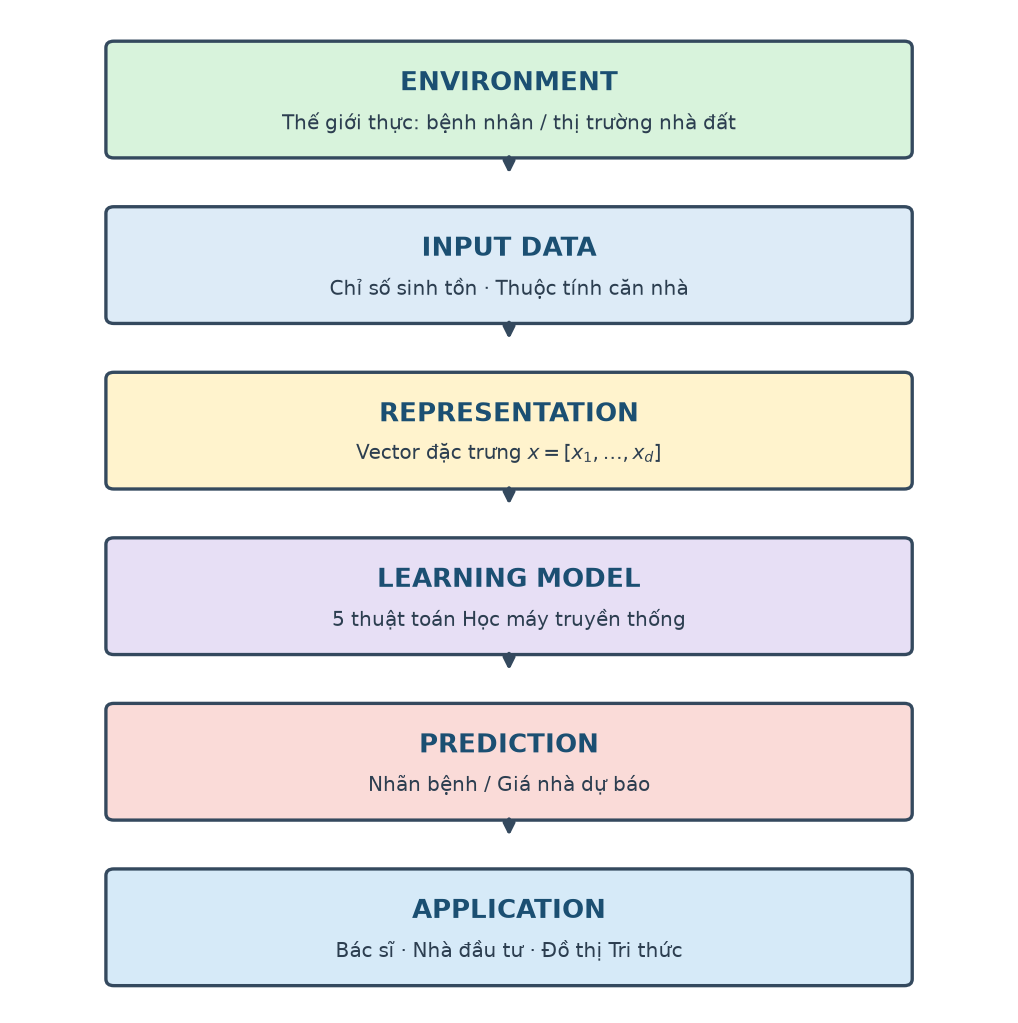
\includegraphics[width=0.54\textwidth]{fig_system_diagram.png}
\caption[Dòng chảy thông tin sáu tầng của một hệ thống thông minh]%
{Dòng chảy thông tin sáu tầng của một hệ thống thông minh, áp dụng đồng thời
cho hệ thống chẩn đoán tiểu đường và hệ thống định giá bất động sản}
\label{fig:sodo-hethong}
\end{figure}

\bieudo{Sơ đồ khối tuần tự (sequential block diagram). Mỗi khối là một tầng xử
lý, mũi tên một chiều thể hiện hướng đi của thông tin; không có vòng lặp ngược
vì đây là kiến trúc suy luận một lượt (single-pass inference), không phải vòng
học tăng cường.}

\nhanxet{Tầng \textsc{Representation} được đặt ở vị trí trung tâm chứ không phải
tầng \textsc{Learning Model}. Đó là một phát biểu có chủ đích của đề bài: mọi
tầng phía sau chỉ thao tác trên véc-tơ đặc trưng, nên bất kỳ thông tin nào bị
đánh mất ở tầng biểu diễn thì không tầng nào sau đó khôi phục lại được.
Mục~\ref{sec:phanchieu} là phần kiểm định thực nghiệm cho nhận định này --- và
kết quả kiểm định không đơn giản như phát biểu.}

\noindent Ánh xạ cụ thể của sáu tầng sang hai bài toán được trình bày ở
Bảng~\ref{tab:sau-tang}.

\begin{table}[H]
\centering
\caption{Ánh xạ sáu tầng kiến trúc sang hai bài toán cụ thể}
\label{tab:sau-tang}
\small
\begin{tabularx}{\textwidth}{@{}L{2.5cm}XX@{}}
\toprule
\textbf{Tầng} & \textbf{Hệ thống 1 --- Tiểu đường} & \textbf{Hệ thống 2 --- Bất động sản} \\
\midrule
Môi trường     & Bệnh nhân đến khám sàng lọc & Thị trường nhà đất Việt Nam \\
Dữ liệu vào    & 768 hồ sơ Pima Indians Diabetes & 30.229 tin đăng rao bán \\
Biểu diễn      & $\mathbf{x}\in\mathbb{R}^{12}$ (8 gốc $+$ 4 thiết kế) & $\mathbf{x}\in\mathbb{R}^{84}$ sau mã hoá one-hot \\
Mô hình học    & 5 bộ phân lớp $+$ 1 mô hình cơ sở & 5 bộ hồi quy $+$ 1 mô hình cơ sở \\
Dự đoán        & Xác suất mắc bệnh $\hat p\in[0,1]$ & Giá dự báo $\hat y$ (tỷ VNĐ) \\
Ứng dụng       & Phân tầng nguy cơ, gói chăm sóc có chi phí & Phân khúc, hạn mức vay và trả góp \\
\bottomrule
\end{tabularx}
\end{table}

\section{Biểu diễn dữ liệu --- bản chất và vai trò}
\label{sec:bieudien}

\subsection{Không gian véc-tơ đặc trưng}

Mọi thuật toán học máy truyền thống đều làm việc trên một không gian số. Cho
tập dữ liệu gồm $n$ quan sát, mỗi quan sát được viết thành một véc-tơ $d$ chiều

\begin{equation}
\mathbf{x}_i = \big[x_{i1},\, x_{i2},\, \dots,\, x_{id}\big]^{\!\top} \in \mathbb{R}^{d},
\qquad i = 1,\dots,n,
\label{eq:vector-dactrung}
\end{equation}

\noindent và toàn bộ tập dữ liệu thành ma trận đặc trưng
$\mathbf{X}\in\mathbb{R}^{n\times d}$ đi kèm véc-tơ nhãn $\mathbf{y}$. Bài toán
học có giám sát là bài toán tìm một hàm $f_{\bm\theta}:\mathbb{R}^{d}\to\mathcal{Y}$
sao cho $f_{\bm\theta}(\mathbf{x})$ xấp xỉ tốt nhãn thật.

Điểm mấu chốt: \emph{hình học của không gian $\mathbb{R}^{d}$ quyết định thuật
toán nhìn thấy gì}. Với K-Nearest Neighbors, khái niệm ``gần nhau'' là khoảng
cách Euclid

\begin{equation}
D(\mathbf{x}_a,\mathbf{x}_b)=\sqrt{\sum_{j=1}^{d}\big(x_{aj}-x_{bj}\big)^{2}}.
\label{eq:euclid}
\end{equation}

\noindent Nếu một cột có thang đo hàng trăm (Insulin, đơn vị $\mu$U/mL) đứng
cạnh một cột có thang đo phần mười (DiabetesPedigreeFunction), thì trong
công thức~\eqref{eq:euclid} cột thứ nhất lấn át hoàn toàn cột thứ hai --- không
phải vì nó quan trọng hơn về mặt y học, mà chỉ vì đơn vị đo của nó lớn hơn. Đây
là lý do bước chuẩn hoá không phải là thủ tục hình thức.

\subsection{Ba tầng chuyển hoá biểu diễn}
\label{sec:ba-tang-bieudien}

Báo cáo phân biệt rõ ba phép biến đổi thường bị gộp chung dưới tên ``tiền xử
lý'', vì Thực nghiệm~3 ở cả hai chương sau đo tác động của chúng một cách
riêng rẽ:

\begin{enumerate}
  \item \textbf{Làm sạch (cleaning).} Sửa lại những giá trị mã hoá sai --- ví
        dụ giá trị $0$ ở cột Glucose không phải nồng độ đường huyết bằng không
        mà là quy ước cho ``không đo được''. Phép này \emph{sửa lại thông tin
        sai lệch}.
  \item \textbf{Thiết kế đặc trưng (feature engineering).} Tạo cột mới từ các
        cột đã có, ví dụ $\mathrm{Glucose}\times\mathrm{BMI}$. Phép này
        \emph{đổi dạng thông tin đã có} --- nó không mang thêm dữ kiện mới nào
        vào hệ thống.
  \item \textbf{Chuẩn hoá (standardisation).} Đưa mọi cột về cùng thang đo:
        \begin{equation}
          z_{ij} = \frac{x_{ij}-\mu_j}{\sigma_j},
          \label{eq:zscore}
        \end{equation}
        với $\mu_j,\sigma_j$ là trung bình và độ lệch chuẩn của cột $j$
        \textbf{học trên riêng tập huấn luyện}. Phép này cũng chỉ
        \emph{đổi dạng}.
\end{enumerate}

Sự phân biệt giữa ``đổi dạng thông tin'' và ``thêm hoặc bớt thông tin'' chính
là chìa khoá giải thích vì sao cùng một thực nghiệm cho hai kết luận trái ngược
trên hai bài toán --- xem Mục~\ref{sec:phanchieu}.

\begin{phathien}{Rò rỉ dữ liệu qua bước tiền xử lý}
Các tham số $\mu_j$, $\sigma_j$ ở công thức~\eqref{eq:zscore}, cũng như giá trị
trung vị dùng để điền khuyết, \textbf{bắt buộc} phải được ước lượng chỉ từ tập
huấn luyện rồi áp lại y nguyên cho tập kiểm tra. Tính trên toàn bộ dữ liệu là
rò rỉ dữ liệu (data leakage)~\cite{kaufman2012}: tập kiểm tra đã gián tiếp góp phần định nghĩa
phép biến đổi mà nó sắp được đánh giá. Trong dự án này, mọi bước tiền xử lý
được gói bên trong đối tượng \texttt{Pipeline} của scikit-learn, nên
\texttt{fit} về mặt cấu trúc không thể nhìn thấy tập kiểm tra.
Mục~\ref{sec:roro} trình bày một trường hợp rò rỉ thật đã xảy ra trong dự án và
hậu quả đo được của nó.
\end{phathien}

\section{Hai lớp bài toán học có giám sát}

\subsection{Phân lớp nhị phân và hàm sigmoid}

Bài toán phân lớp nhị phân có $\mathcal{Y}=\{0,1\}$. Hồi quy Logistic mô hình
hoá \emph{xác suất} thuộc lớp dương bằng cách đưa một tổ hợp tuyến tính qua
hàm sigmoid (còn gọi là hàm logistic)~\cite{bishop2006}:

\begin{equation}
\sigma(z) = \frac{1}{1+e^{-z}}, \qquad z \in \mathbb{R},
\label{eq:sigmoid}
\end{equation}

\begin{equation}
\hat p(\mathbf{x}) \;=\; P(y=1\mid \mathbf{x})
\;=\; \sigma\!\big(\mathbf{w}^{\!\top}\mathbf{x}+b\big)
\;=\; \frac{1}{1+\exp\!\big[-(\mathbf{w}^{\!\top}\mathbf{x}+b)\big]}.
\label{eq:logistic}
\end{equation}

\noindent Hàm $\sigma$ ép mọi số thực về khoảng $(0,1)$, đơn điệu tăng, đối
xứng qua điểm $(0,\,0{,}5)$, và có đạo hàm
$\sigma'(z)=\sigma(z)\big[1-\sigma(z)\big]$ --- tính chất khiến việc tối ưu
bằng gradient trở nên gọn gàng.

Hàm mất mát tương ứng là entropy chéo nhị phân (binary cross-entropy, còn gọi
là log-loss):

\begin{equation}
\mathcal{L}_{\mathrm{log}}(\bm\theta)
= -\frac{1}{n}\sum_{i=1}^{n}
\Big[\, y_i \log \hat p_i \;+\; (1-y_i)\log\big(1-\hat p_i\big) \Big].
\label{eq:logloss}
\end{equation}

\subsection{Hồi quy và hàm mất mát bình phương sai số}

Bài toán hồi quy có $\mathcal{Y}=\mathbb{R}$. Hàm mất mát chuẩn là sai số bình
phương trung bình:

\begin{equation}
\mathcal{L}_{\mathrm{MSE}}(\bm\theta)
= \frac{1}{n}\sum_{i=1}^{n}\big(y_i - \hat y_i\big)^{2},
\qquad \hat y_i = f_{\bm\theta}(\mathbf{x}_i).
\label{eq:mse}
\end{equation}

\subsection{Hàm mất mát có điều chuẩn}

Cực tiểu hoá trần các hàm~\eqref{eq:logloss} hoặc~\eqref{eq:mse} dễ dẫn tới học
thuộc (overfitting): mô hình khớp cả nhiễu của tập huấn luyện. Điều chuẩn
(regularisation) thêm một số hạng phạt vào độ lớn tham số~\cite{hastie2009}:

\begin{equation}
\mathcal{J}(\bm\theta)
\;=\; \underbrace{\frac{1}{n}\sum_{i=1}^{n} \ell\big(y_i,\, f_{\bm\theta}(\mathbf{x}_i)\big)}_{\text{sai số trên dữ liệu}}
\;+\; \underbrace{\lambda \,\lVert \bm\theta \rVert_{2}^{2}}_{\text{số hạng điều chuẩn } L_2},
\qquad
\lVert \bm\theta \rVert_{2}^{2}=\sum_{j=1}^{d}\theta_j^{2}.
\label{eq:regularized}
\end{equation}

\noindent Tham số $\lambda>0$ điều tiết đánh đổi giữa khớp dữ liệu và giữ mô
hình đơn giản. Trong scikit-learn~\cite{scikit2011}, \texttt{LogisticRegression} mặc định dùng
phạt $L_2$ với $C=1/\lambda=1$ --- chi tiết này sẽ trực tiếp giải thích một kết
quả phản trực giác ở Mục~\ref{sec:dactrung-tot}, nơi một đặc trưng thiết kế
\emph{tốt} lại làm Hồi quy Logistic \emph{kém đi}.

\section{Nguyên lý mô hình cơ sở}
\label{sec:baseline}

Một con số độ đo đứng một mình không mang thông tin. Accuracy $0{,}79$ là tốt
hay tồi phụ thuộc hoàn toàn vào việc đoán mù đạt bao nhiêu. \textbf{Mô hình cơ
sở} (baseline) là quy tắc đơn giản nhất có thể, không học gì từ đặc trưng, đóng
vai trò mốc so sánh bắt buộc (yêu cầu R6 của đề bài):

\begin{itemize}
  \item \textbf{Phân lớp} --- luôn đoán lớp chiếm đa số
        (\texttt{DummyClassifier(strategy="most\_frequent")}).
  \item \textbf{Hồi quy} --- luôn đoán trung vị của tập huấn luyện
        (\texttt{DummyRegressor(strategy="median")}).
\end{itemize}

Ở bài toán tiểu đường, mô hình cơ sở đạt Accuracy $0{,}6547$ --- một con số
thoạt nhìn không tệ --- nhưng Recall bằng $0$, tức \emph{bỏ sót toàn bộ người
bệnh}. Đây là minh hoạ trực tiếp cho nghịch lý Accuracy trên dữ liệu lệch lớp,
và là lý do mọi kết luận trong Chương~\ref{ch:tieuduong} đều căn theo $F_1$ và
Recall chứ không căn theo Accuracy.

\section{Sáu họ thuật toán học máy sử dụng}

Năm mô hình cho mỗi bài toán được chọn theo tiêu chí \emph{khác nhau về nguyên
lý học}, để phép so sánh nói lên điều gì đó về bản chất dữ liệu chứ không chỉ
so sánh các biến thể của cùng một ý tưởng.

\begin{table}[H]
\centering
\caption{Nguyên lý học, giả định và siêu tham số của các thuật toán sử dụng}
\label{tab:thuattoan}
\scriptsize
\begin{tabularx}{\textwidth}{@{}L{2.3cm}XL{2.95cm}@{}}
\toprule
\textbf{Thuật toán} & \textbf{Nguyên lý học và giả định} & \textbf{Siêu tham số dùng} \\
\midrule
Linear Regression &
Khớp siêu phẳng cực tiểu hoá~\eqref{eq:mse}. Giả định quan hệ tuyến tính giữa đặc trưng và mục tiêu; trần hiệu năng bị chặn bởi độ mạnh tương quan tuyến tính. &
Mặc định \\
\addlinespace
Logistic Regression &
Ranh giới tuyến tính trong không gian log-odds qua~\eqref{eq:logistic}, phạt $L_2$ theo~\eqref{eq:regularized}. Nhạy với đa cộng tuyến. &
\texttt{max\_iter=1000} \\
\addlinespace
K-Nearest Neighbors &
Không học tham số~\cite{cover1967}; nhãn quyết định bởi $k$ láng giềng gần nhất theo~\eqref{eq:euclid}. \textbf{Bắt buộc} chuẩn hoá. &
\texttt{n\_neighbors=11} \\
\addlinespace
Decision Tree &
Chia đệ quy không gian đặc trưng bằng ngưỡng trên từng trục, cực tiểu hoá độ vẩn (Gini hoặc MSE). Bất biến với phép chuẩn hoá đơn điệu. &
\texttt{max\_depth=6} (phân lớp), \texttt{12} (hồi quy) \\
\addlinespace
Random Forest &
Tổng hợp nhiều cây trên mẫu bootstrap~\cite{breiman2001} cộng với chọn ngẫu nhiên tập con đặc trưng; giảm phương sai bằng trung bình hoá. &
\texttt{n\_estimators=300/200}, \texttt{max\_depth=10/18}, \texttt{min\_samples\_leaf=5} \\
\addlinespace
Support Vector Regression &
Tìm ống $\varepsilon$ mỏng nhất chứa phần lớn điểm~\cite{cortes1995}; độ phức tạp bậc hai theo số mẫu. &
\texttt{C=10.0}, \texttt{epsilon=0.2} \\
\addlinespace
XGBoost &
Cộng dồn tuần tự các cây yếu~\cite{chen2016}, mỗi cây sửa phần dư của tổ hợp trước đó; có điều chuẩn nội tại. &
\texttt{n\_estimators=300/500}, \texttt{max\_depth=4/6}, \texttt{learning\_rate=0.05} \\
\bottomrule
\end{tabularx}
\end{table}

\section{Hệ thống độ đo đánh giá}
\label{sec:dodo}

\subsection{Ma trận nhầm lẫn và bốn độ đo phân lớp}

Với bài toán nhị phân, đối chiếu nhãn thật và nhãn dự đoán cho bốn ô của
\textbf{ma trận nhầm lẫn} (Bảng~\ref{tab:confusion-schema}).

\begin{table}[H]
\centering
\caption{Ma trận nhầm lẫn --- ý nghĩa lâm sàng của từng ô}
\label{tab:confusion-schema}
\small
\begin{tabularx}{\textwidth}{@{}L{2.1cm}L{2.6cm}X@{}}
\toprule
\textbf{Ký hiệu} & \textbf{Tên} & \textbf{Ý nghĩa trong bài toán chẩn đoán} \\
\midrule
TP & Dương tính thật & Người bệnh, được phát hiện đúng \\
TN & Âm tính thật    & Người khoẻ, được kết luận đúng \\
FP & Dương tính giả  & Người khoẻ bị báo động nhầm --- tốn thêm một lần xét nghiệm \\
FN & Âm tính giả     & \textbf{Người bệnh bị bỏ sót} --- sai lầm nghiêm trọng nhất \\
\bottomrule
\end{tabularx}
\end{table}

Bốn độ đo chuẩn được định nghĩa từ bốn ô này:

\begin{align}
\text{Accuracy}  &= \frac{TP+TN}{TP+TN+FP+FN}, \label{eq:accuracy}\\[4pt]
\text{Precision} &= \frac{TP}{TP+FP}, \label{eq:precision}\\[4pt]
\text{Recall}    &= \frac{TP}{TP+FN}, \label{eq:recall}\\[4pt]
F_1 &= 2\cdot\frac{\text{Precision}\cdot\text{Recall}}
                  {\text{Precision}+\text{Recall}}. \label{eq:f1}
\end{align}

\noindent Cách đọc bốn công thức trên trong ngữ cảnh y tế:

\begin{itemize}
  \item \textbf{Accuracy}~\eqref{eq:accuracy} --- tỷ lệ đúng chung. Mất ý nghĩa
        khi hai lớp lệch nhau: ở tập Pima, đoán ``tất cả đều khoẻ'' đã đạt
        $65{,}5\%$.
  \item \textbf{Precision}~\eqref{eq:precision} --- trong những ca bị báo động,
        bao nhiêu phần trăm là báo động thật. Precision thấp nghĩa là hệ thống
        gây phiền nhiễu.
  \item \textbf{Recall}~\eqref{eq:recall} --- trong toàn bộ người bệnh, bao
        nhiêu phần trăm được tìm ra. \textbf{Đây là độ đo quan trọng nhất của
        bài toán sàng lọc}, vì FN là sai lầm đắt nhất.
  \item $F_1$~\eqref{eq:f1} --- trung bình điều hoà của hai độ đo trên. Trung
        bình điều hoà (chứ không phải trung bình cộng) phạt nặng trường hợp một
        trong hai độ đo gần $0$: mô hình cơ sở có Precision $=$ Recall $=0$ nên
        $F_1=0$, phản ánh đúng thực chất.
\end{itemize}

Ngoài bốn độ đo trên, báo cáo dùng \textbf{ROC-AUC} --- diện tích dưới đường
cong biểu diễn Recall theo tỷ lệ Dương tính giả khi ngưỡng quyết định quét từ
$1$ về $0$. ROC-AUC~\cite{fawcett2006} đo \emph{khả năng xếp hạng} của mô hình và độc lập
với ngưỡng, nên nó là độ đo duy nhất trong nhóm không thay đổi khi ta chỉnh ngưỡng
ở Thực nghiệm~1.

\subsection{Ba độ đo hồi quy}

\begin{align}
\text{MAE}  &= \frac{1}{n}\sum_{i=1}^{n}\big| y_i - \hat y_i \big|, \label{eq:mae}\\[4pt]
\text{RMSE} &= \sqrt{\frac{1}{n}\sum_{i=1}^{n}\big( y_i - \hat y_i \big)^{2}}, \label{eq:rmse}\\[4pt]
R^{2} &= 1 - \frac{\sum_{i=1}^{n}\big( y_i - \hat y_i \big)^{2}}
                  {\sum_{i=1}^{n}\big( y_i - \bar y \big)^{2}}. \label{eq:r2}
\end{align}

\noindent MAE~\eqref{eq:mae} giữ nguyên đơn vị của biến mục tiêu, nên
``MAE $=1{,}05$'' đọc thẳng được là ``sai trung bình $1{,}05$ tỷ đồng mỗi căn''.
RMSE~\eqref{eq:rmse} bình phương sai số trước khi lấy trung bình nên phạt nặng
các ca sai lớn; khoảng cách giữa RMSE và MAE do đó là một chỉ báo về mức độ tồn
tại của các ca sai cực đoan. $R^{2}$~\eqref{eq:r2} là tỷ lệ phương sai của biến
mục tiêu được mô hình giải thích: $R^{2}=1$ là dự báo hoàn hảo, $R^{2}=0$ là
ngang với việc luôn đoán giá trị trung bình, và $R^{2}<0$ nghĩa là mô hình còn
tệ hơn cả đoán trung bình.

\begin{phathien}{$R^2$ không so sánh được giữa hai tập dữ liệu khác nhau}
Mẫu số của~\eqref{eq:r2} là phương sai của chính biến mục tiêu. Nếu một tập dữ
liệu có mục tiêu bị thu hẹp dải giá trị --- đúng trường hợp của tập bất động
sản, xem Mục~\ref{sec:price-cat-bien} --- thì mẫu số nhỏ đi và cùng một sai số
tuyệt đối sẽ cho $R^{2}$ thấp hơn. Do đó $R^{2}=0{,}61$ ở đây khắt khe hơn con
số $0{,}61$ trên một tập có dải giá trải rộng.
\end{phathien}

\section{Đồ thị Tri thức}
\label{sec:kg-lythuyet}

\subsection{Giới hạn cố hữu của mô hình hộp đen}

Một mô hình học máy được huấn luyện tốt trả lời được câu hỏi ``bao nhiêu'' và
``khả năng nào'', nhưng không trả lời được ``vì vậy thì phải làm gì''. Xác suất
$0{,}545$ không tự nó nói cho bác sĩ biết cần chỉ định xét nghiệm nào, cũng
không nói cho người bệnh biết phải mua máy đo nào và tốn bao nhiêu; con số
$8{,}42$ tỷ không tự nó nói cho người mua biết ngân hàng cho vay tối đa bao
nhiêu và mỗi tháng phải trả bao nhiêu. Khoảng trống giữa \emph{con số dự báo} và
\emph{hành động cụ thể} là khoảng trống mà tri thức miền phải lấp, và Đồ thị Tri
thức là cấu trúc dữ liệu để mã hoá tri thức ấy dưới dạng máy suy luận được.

\subsection{Định nghĩa hình thức}

Một \textbf{Đồ thị Tri thức}~\cite{hogan2021,ji2022} là bộ ba

\begin{equation}
\mathcal{KG} \;=\; \big(V,\; E,\; R\big),
\label{eq:kg}
\end{equation}

\noindent trong đó $V$ là tập \emph{thực thể} (đỉnh), $R$ là tập \emph{loại
quan hệ}, và $E\subseteq V\times R\times V$ là tập \emph{cạnh có nhãn}. Mỗi
phần tử của $E$ là một \textbf{bộ ba tri thức} (knowledge triplet)

\begin{equation}
\big(h,\; r,\; t\big) \in E,
\qquad h,t \in V,\; r \in R,
\label{eq:triplet}
\end{equation}

\noindent đọc là ``chủ thể $h$ có quan hệ $r$ với đối tượng $t$''. Ví dụ thật
lấy từ đồ thị của hệ thống thứ nhất:

\begin{center}
\small
\begin{tabular}{@{}l@{}}
\texttt{(Bệnh nhân \#192, HAS\_BIOMARKER, Glucose = 159 mg/dL)}\\
\texttt{(Mô hình K-Nearest Neighbors, PRODUCES, Xác suất rủi ro 54.5\%)}\\
\texttt{(Xác suất rủi ro 54.5\%, MAPS\_TO\_DISEASE, ICD-10 E11)}\\
\texttt{(Nhóm Nguy cơ Cao, RECOMMENDS\_PACKAGE, Gói Theo dõi Chuyên sâu)}\\
\texttt{(Gói Theo dõi Chuyên sâu, FULFILLED\_BY, Nhà thuốc FPT Long Châu)}\\
\end{tabular}
\end{center}

Năm bộ ba trên nối liền một mạch từ số đo sinh học tới nơi mua được hàng ---
năng lực mà mô hình đơn lẻ không có. Đồ thị của dự án này có $|V|=117$,
$|E|=133$ và $|R|=28$ trên 6 ca mẫu, đã nạp thật lên máy chủ Neo4j Aura.

\subsection{Kiến trúc năm tầng}
\label{sec:kg-5-tang}

Bộ ba $(V,E,R)$ ở~\eqref{eq:kg} mô tả \emph{cấu trúc}, nhưng không nói gì về
\emph{tổ chức}. Đồ thị của dự án này được tổ chức thành năm tầng ở cả hai miền
--- Hình~\ref{fig:kg-arch-medical} và Hình~\ref{fig:kg-arch-property}. Mỗi tầng
là một nhóm loại thực thể, và thông tin chỉ chảy theo một chiều từ tầng trên
xuống tầng dưới.

\begin{figure}[H]
\centering
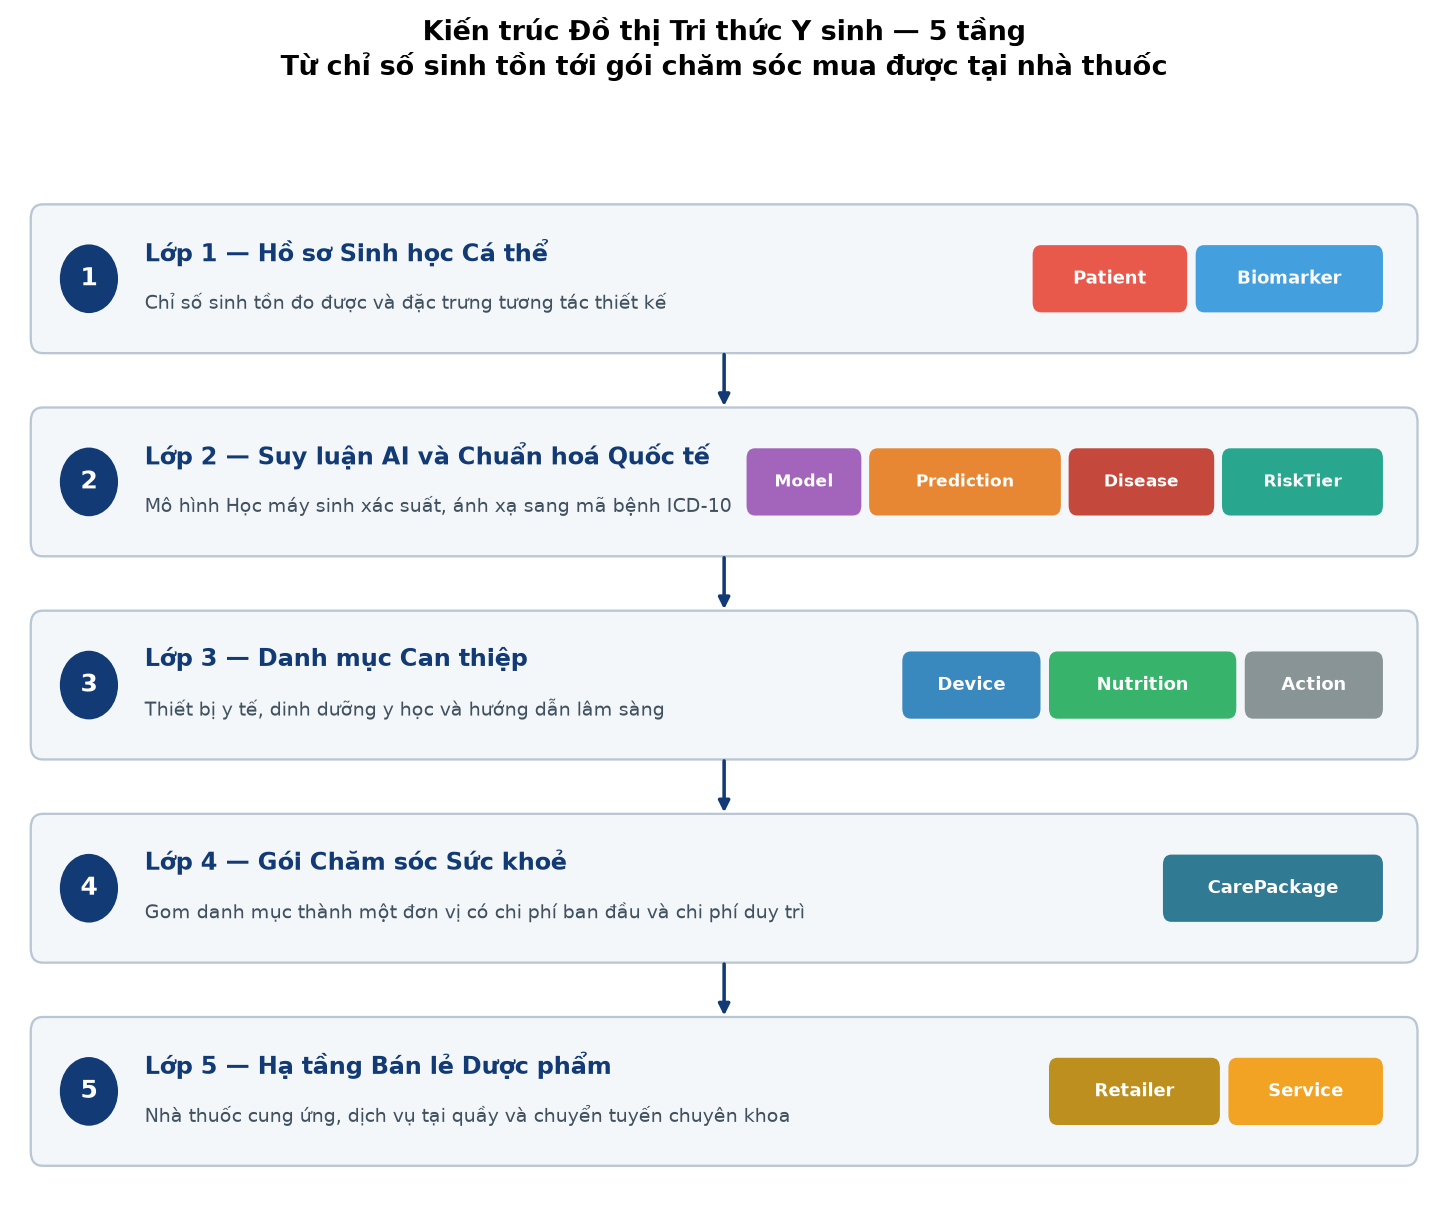
\includegraphics[width=\textwidth]{fig_kg_architecture_medical.png}
\caption[Kiến trúc năm tầng của Đồ thị Tri thức Y sinh]%
{Kiến trúc năm tầng của Đồ thị Tri thức Y sinh --- từ chỉ số sinh tồn tới gói
chăm sóc mua được tại nhà thuốc}
\label{fig:kg-arch-medical}
\end{figure}

\begin{figure}[H]
\centering
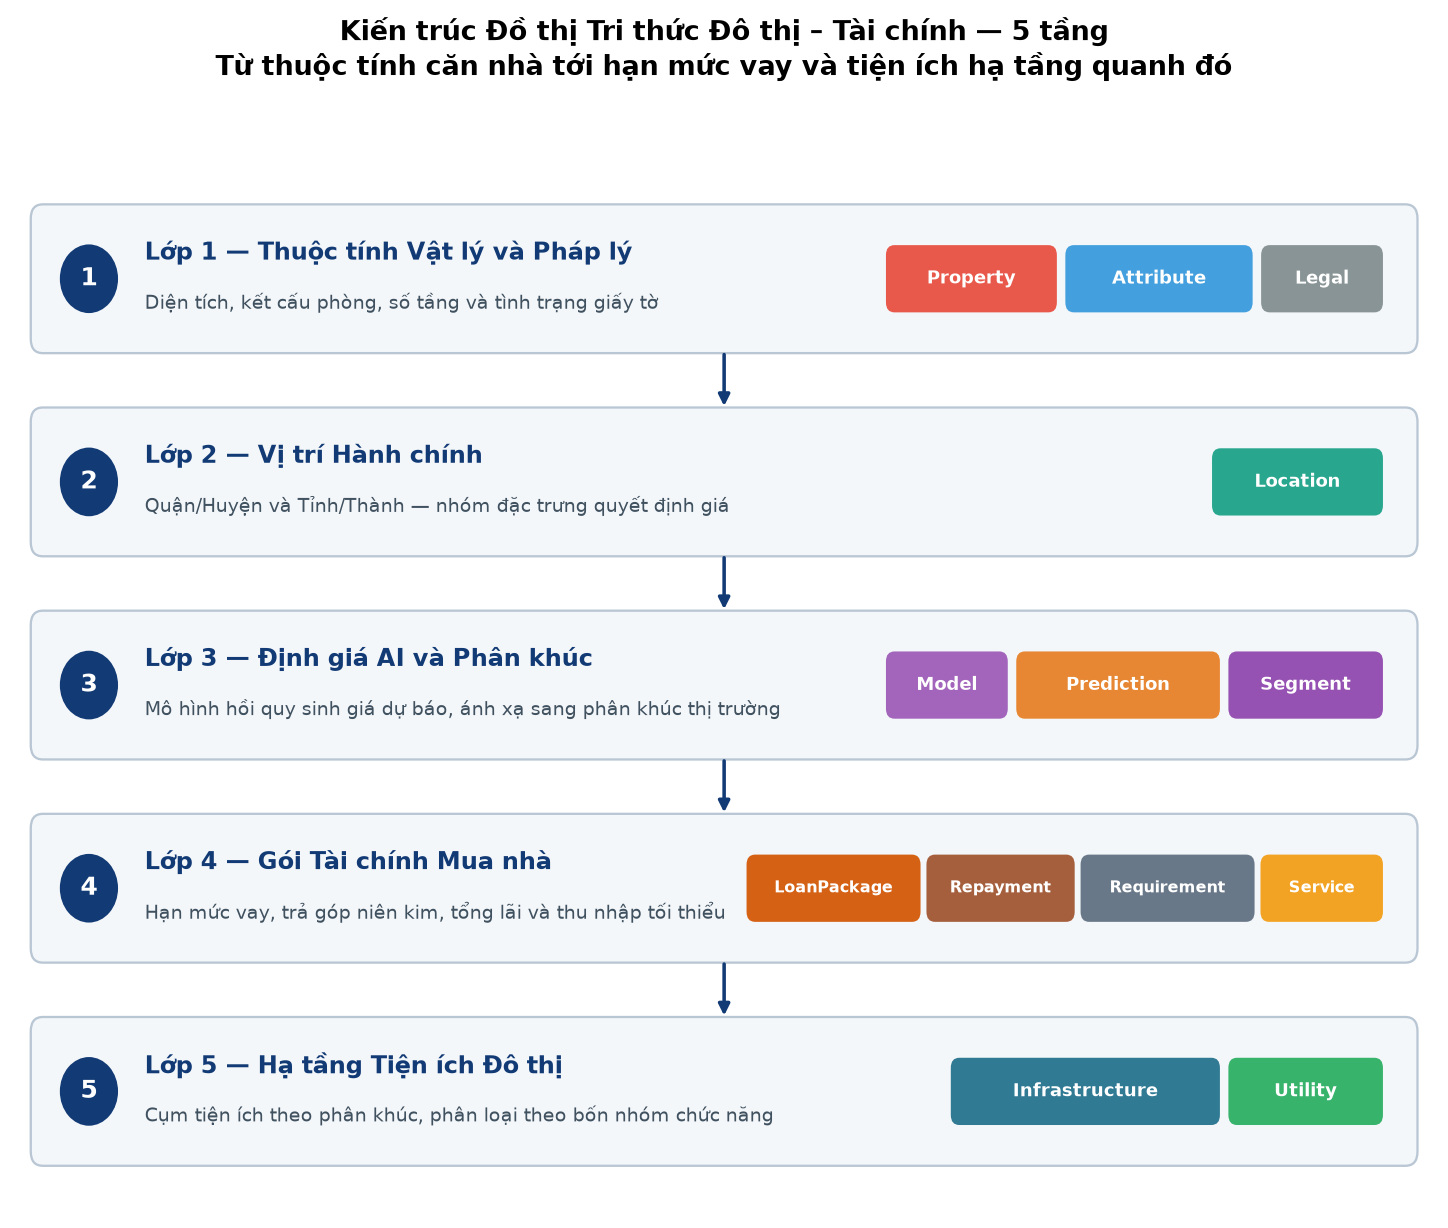
\includegraphics[width=\textwidth]{fig_kg_architecture_property.png}
\caption[Kiến trúc năm tầng của Đồ thị Tri thức Đô thị -- Tài chính]%
{Kiến trúc năm tầng của Đồ thị Tri thức Đô thị -- Tài chính --- từ thuộc tính
căn nhà tới hạn mức vay và tiện ích hạ tầng quanh đó}
\label{fig:kg-arch-property}
\end{figure}

\bieudo{Sơ đồ tầng (layered schema diagram). Khác với ảnh chụp đồ thị của một
ca cụ thể ở Hình~\ref{fig:kg-medical} và Hình~\ref{fig:kg-property} --- vốn cho
thấy \emph{dữ liệu} --- hai hình trên cho thấy \emph{lược đồ}: đồ thị có mấy
tầng, mỗi tầng chứa loại thực thể nào, thông tin chảy theo hướng nào.}

\nhanxet{Hai kiến trúc song song nhau đến từng tầng, và đó là thiết kế có chủ
đích. Tầng 1--2 là \emph{quan sát}, tầng 3 là \emph{suy luận của mô hình}, tầng
4 là \emph{gói giải pháp có chi phí}, tầng 5 là \emph{hạ tầng cung ứng}. Nhờ
cùng khung, một câu hỏi đặt ra ở miền này luôn có câu hỏi đối ứng ở miền kia:
``gói chăm sóc tốn bao nhiêu mỗi tháng'' đối ứng với ``khoản vay trả góp bao
nhiêu mỗi tháng''.

Hai hình trên được vẽ tự động từ chính khai báo \texttt{KG\_LAYERS} trong
\texttt{src/kg/ontology.py}, nên chúng không thể mô tả một kiến trúc mà mã nguồn
không còn dùng. Một bài kiểm thử canh đúng điều đó: mọi loại thực thể mà mã
nguồn thật sự sinh ra đều phải thuộc đúng một tầng.}

\subsection{Ba vai trò của đồ thị trong hệ thống}

\begin{enumerate}
  \item \textbf{Diễn giải (interpretability).} Đường đi từ đỉnh ``Bệnh nhân''
        tới đỉnh ``Gói chăm sóc'' là một chuỗi bước đọc được bằng ngôn ngữ tự
        nhiên, khác hẳn trọng số của một cây tăng cường.
  \item \textbf{Nối tri thức miền.} Bảng phân loại ICD-10~\cite{icd10}, ngưỡng BMI của WHO~\cite{who2000},
        danh mục hàng của nhà thuốc, tỷ lệ LTV và ngưỡng DTI của ngân hàng ---
        những tri thức này không có trong dữ liệu huấn luyện và cũng không nên
        học từ dữ liệu; chúng được khai báo tường minh thành đỉnh và cạnh.
  \item \textbf{Sinh hành động có chi phí.} Truy vấn đồ thị theo tầng nguy cơ
        hoặc phân khúc giá trả về ngay một gói kèm con số: chi phí ban đầu, chi
        phí duy trì hằng tháng, hoặc khoản trả góp và mức thu nhập tối thiểu.
        Đây chính là đầu ra của tầng \textsc{Application} ở
        Hình~\ref{fig:sodo-hethong}.
\end{enumerate}

\subsection{Ranh giới trung thực về nguồn số liệu}
\label{sec:ranh-gioi-so-lieu}

Hai tầng cuối của mỗi đồ thị chứa số liệu \emph{không} đến từ tập dữ liệu huấn
luyện, nên nguồn gốc của chúng phải được nói rõ chứ không được trình bày lẫn
với kết quả đo được:

\begin{itemize}
  \item \textbf{Tên mặt hàng là tên thật} đang được bán tại hệ thống nhà thuốc.
        \textbf{Giá là khoảng tham khảo có ghi ngày chốt} (26/08/2026), biên
        soạn tay từ danh mục công khai --- không phải bản ghi giá trực tiếp. Mỗi
        mặt hàng mang theo một đường dẫn tra cứu để người dùng đối chiếu giá
        hiện hành.
  \item \textbf{Cụm tiện ích đô thị được mô hình hoá theo phân khúc}, không
        phải kết quả khảo sát thực địa từng quận: tập dữ liệu gốc chỉ có địa chỉ
        hành chính, không có toạ độ.
  \item \textbf{Điều kiện vay là minh hoạ} theo mặt bằng lãi suất công bố, không
        phải chào giá của một ngân hàng cụ thể. Ngược lại, \emph{phép tính} trả
        góp là toán học thuần tuý và kiểm chứng được --- xem
        Mục~\ref{sec:cong-thuc-nien-kim}.
\end{itemize}

Phương án thu thập giá trực tiếp từ website bán lẻ đã được cân nhắc và bị loại,
vì nó phá vỡ yêu cầu R14 về tính tái lập: giá đổi theo ngày nên hai lần chạy
cách nhau một tuần sẽ cho hai bộ số khác nhau, trong khi cả báo cáo được xây
trên cam kết ``chạy lại cho kết quả trùng khít''.

\subsection{Phép tính tài chính}
\label{sec:cong-thuc-nien-kim}

Khoản trả góp cố định hằng tháng của một khoản vay niên kim là

\begin{equation}
M \;=\; P \cdot \frac{r}{1-(1+r)^{-n}},
\qquad r=\frac{r_{\text{năm}}}{12},\quad n = 12\,T,
\label{eq:nienkim}
\end{equation}

\noindent với $P$ là dư nợ gốc, $r_{\text{năm}}$ là lãi suất danh nghĩa theo
năm và $T$ là kỳ hạn tính bằng năm. Tổng tiền lãi phải trả trong toàn bộ kỳ hạn
là $Mn - P$. Mức thu nhập tối thiểu suy ra từ ngưỡng tỷ lệ nợ trên thu nhập
(Debt-To-Income):

\begin{equation}
I_{\min} \;=\; \frac{M}{\text{DTI}_{\max}}.
\label{eq:dti}
\end{equation}

Ba công thức này được kiểm thử tự động bằng một phép tính độc lập viết lại tay,
chứ không đối chiếu với chính hàm cần kiểm.

\section{Giao thức thực nghiệm chung}
\label{sec:giaothuc}

Hai chương sau dùng chung một giao thức, để mọi so sánh giữa hai bài toán là so
sánh công bằng.

\subsection{Chia dữ liệu ba phần}

Dữ liệu được cắt làm ba, theo đúng thứ tự sau:

\begin{enumerate}
  \item \textbf{Tập ngoại kiểm (OOD), $10\%$} --- cắt ra \emph{trước tiên} và
        không tham gia bất kỳ bước nào của quá trình phát triển, kể cả tinh
        chỉnh siêu tham số.
  \item \textbf{Tập kiểm tra, $20\%$ phần còn lại} --- dùng để so sánh mô hình.
  \item \textbf{Tập huấn luyện, phần còn lại} --- dùng để học tham số.
\end{enumerate}

Lý do tách riêng tập ngoại kiểm: sau nhiều vòng thử nghiệm, tập kiểm tra thông
thường đã \emph{gián tiếp} ảnh hưởng tới lựa chọn mô hình, nên nó không còn là
ước lượng không chệch của hiệu năng thực tế. Tập ngoại kiểm đóng vai trò ``dữ
liệu thế giới thực'' chưa từng bị nhìn thấy.

\subsection{Bốn thực nghiệm có kiểm soát}

Mỗi bài toán chạy bốn thực nghiệm cùng khuôn (đề bài yêu cầu tối thiểu ba ---
R8), mỗi thực nghiệm chỉ đổi \emph{một} biến và giữ nguyên mọi thứ còn lại:

\begin{table}[H]
\centering
\caption{Bốn thực nghiệm có kiểm soát, áp dụng song song cho hai bài toán}
\label{tab:bon-thucnghiem}
\small
\begin{tabularx}{\textwidth}{@{}L{0.8cm}L{3.5cm}XL{2.3cm}@{}}
\toprule
\textbf{TN} & \textbf{Biến được thay đổi} & \textbf{Câu hỏi trả lời} & \textbf{Kết quả ở} \\
\midrule
1 & Đối đầu 5 thuật toán & Nguyên lý học nào hợp với dữ liệu này? & \ref{sec:tn1-dia}, \ref{sec:tn1-hou} \\
2 & Siêu tham số cốt lõi & Cực trị nằm ở đâu, có chạm biên dải khảo sát không? & \ref{sec:tn2-dia}, \ref{sec:tn2-hou} \\
3 & Cách biểu diễn dữ liệu & Biểu diễn hay thuật toán chi phối kết quả? & \ref{sec:tn3-dia}, \ref{sec:tn3-hou} \\
4 & Tập đánh giá (kiểm tra $\to$ ngoại kiểm) & Mô hình tổng quát hoá được tới đâu? & \ref{sec:tn4-dia}, \ref{sec:tn4-hou} \\
\bottomrule
\end{tabularx}
\end{table}

\subsection{Tính tái lập}
\label{sec:tailap}

Hạt giống ngẫu nhiên cố định tại \texttt{RANDOM\_STATE = 42} khai báo một lần
duy nhất trong \texttt{src/config.py} và được mọi thành phần dùng lại. Một lệnh
\texttt{python run\_pipeline.py} sinh lại toàn bộ mô hình, biểu đồ, bảng số và
đồ thị tri thức trong khoảng 90 giây.

Một lưu ý trung thực về mức độ tái lập: các tệp \texttt{models/*.joblib} chạy
lại cho kết quả trùng khít, nhưng vài tệp CSV của bài toán bất động sản có thể
lệch ở chữ số cuối của số thực (bậc $10^{-16}$) --- ví dụ MAE của Random Forest
đổi từ $1{,}0818214861905244$ thành $1{,}0818214861905247$. Nguyên nhân là phép
cộng dồn song song trong rừng ngẫu nhiên không có tính kết hợp. Ở độ chính xác
báo cáo --- bốn chữ số thập phân --- mọi con số đều trùng khớp.

% =====================================================================
%  Chương 2 — Hệ thống Chẩn đoán Nguy cơ Tiểu đường
% =====================================================================
\chapter{Hệ thống Chẩn đoán Nguy cơ Tiểu đường}
\label{ch:tieuduong}

\section{Phát biểu bài toán}
\label{sec:phatbieu-dia}

\subsection{Hiện tượng thực tế và người dùng}

Đái tháo đường type 2 tiến triển âm thầm: người bệnh thường không có triệu
chứng rõ rệt cho tới khi biến chứng đã hình thành. Vì vậy giá trị của một hệ
thống trong miền này không nằm ở chỗ ``chẩn đoán chính xác'' --- việc ấy thuộc
về xét nghiệm HbA1c tĩnh mạch --- mà nằm ở chỗ \textbf{sàng lọc}: từ những chỉ
số đo được rẻ và nhanh, chỉ ra ai cần đi làm xét nghiệm khẳng định.

Việc xác định đúng vai trò này quyết định mọi lựa chọn kỹ thuật về sau. Nó là
lý do báo cáo chấm điểm bằng $F_1$ và Recall chứ không bằng Accuracy
(Mục~\ref{sec:baseline}), và là lý do Thực nghiệm~2 hạ ngưỡng quyết định xuống
tận $0{,}15$ (Mục~\ref{sec:tn2-dia}).

\subsection{Phát biểu hình thức}

Cho một hồ sơ y sinh $\mathbf{x}\in\mathbb{R}^{d}$ gồm các chỉ số đo được của
một người, hãy học hàm

\begin{equation}
f_{\bm\theta}:\ \mathbb{R}^{d}\longrightarrow[0,1],
\qquad
\hat p = f_{\bm\theta}(\mathbf{x}) = P\big(\texttt{Outcome}=1 \mid \mathbf{x}\big),
\label{eq:baitoan-dia}
\end{equation}

\noindent rồi quy xác suất về nhãn nhị phân qua một ngưỡng quyết định $\theta$:

\begin{equation}
\hat y = \mathbb{1}\big[\,\hat p \ge \theta\,\big],
\qquad \theta \in (0,1).
\label{eq:nguong-dia}
\end{equation}

Ngưỡng $\theta$ ở~\eqref{eq:nguong-dia} là một tham số \textbf{của hệ thống},
không phải của mô hình: nó không được học từ dữ liệu mà được chọn theo mục tiêu
sử dụng. Việc tách bạch hai thứ này là điều kiện cần để Thực nghiệm~2 có nghĩa.

\begin{table}[H]
\centering
\caption{Đặc tả bài toán chẩn đoán nguy cơ tiểu đường}
\label{tab:dacta-dia}
\small
\begin{tabularx}{\textwidth}{@{}L{4.2cm}X@{}}
\toprule
\textbf{Hạng mục} & \textbf{Nội dung} \\
\midrule
Hiện tượng thực tế   & Tình trạng chuyển hoá glucose và nguy cơ mắc đái tháo đường type 2 \\
Một quan sát         & Một hồ sơ y sinh của một người trưởng thành \\
Loại bài toán        & Phân lớp nhị phân (Binary Classification) \\
Biến mục tiêu        & \texttt{Outcome} $\in\{0,1\}$ \\
Số quan sát          & 768 hồ sơ \\
Đặc trưng đầu vào    & 8 cột gốc, tất cả đều là số; không có biến định danh \\
Đặc trưng sau thiết kế & 12 cột (8 gốc $+$ 4 phái sinh) \\
Người dùng cuối      & Bác sĩ sàng lọc, và chính người được sàng lọc \\
Độ đo quyết định     & $F_1$ và Recall --- không phải Accuracy \\
\bottomrule
\end{tabularx}
\end{table}

\section{Tập dữ liệu và nguồn gốc}
\label{sec:dulieu-dia}

Tập \textbf{Pima Indians Diabetes}~\cite{pima} do Viện Quốc gia về Đái tháo đường, Bệnh
Tiêu hoá và Bệnh Thận Hoa Kỳ thu thập, công bố công khai trên Kaggle:

\begin{center}
\small\url{https://www.kaggle.com/datasets/uciml/pima-indians-diabetes-database}
\end{center}

Toàn bộ đối tượng là nữ, từ 21 tuổi trở lên, thuộc cộng đồng người Pima --- một
giới hạn về phạm vi áp dụng sẽ được nêu lại ở Mục~\ref{sec:hanche}.

\begin{table}[H]
\centering
\caption{Đặc tả tám đặc trưng gốc của tập Pima Indians Diabetes}
\label{tab:dactrung-dia}
\small
\begin{tabularx}{\textwidth}{@{}L{3.5cm}L{1.6cm}R{1.5cm}R{1.5cm}X@{}}
\toprule
\textbf{Đặc trưng} & \textbf{Đơn vị} & \textbf{Trung bình} & \textbf{Trung vị} & \textbf{Ý nghĩa} \\
\midrule
Pregnancies              & lần   & 3{,}845   & 3{,}0   & Số lần mang thai \\
Glucose                  & mg/dL & 121{,}656 & 117{,}0 & Đường huyết sau nghiệm pháp dung nạp 2 giờ \\
BloodPressure            & mmHg  & 72{,}387  & 72{,}0  & Huyết áp tâm trương \\
SkinThickness            & mm    & 29{,}108  & 29{,}0  & Độ dày nếp gấp da cơ tam đầu \\
Insulin                  & $\mu$U/mL & 140{,}672 & 125{,}0 & Insulin huyết thanh sau 2 giờ \\
BMI                      & kg/m$^2$ & 32{,}455 & 32{,}3 & Chỉ số khối cơ thể \\
DiabetesPedigreeFunction & --    & 0{,}472   & 0{,}372 & Chỉ số di truyền gia đình \\
Age                      & năm   & 33{,}241  & 29{,}0  & Tuổi \\
\bottomrule
\end{tabularx}
\end{table}

\nhanxet{Trung bình lớn hơn trung vị ở hầu hết các cột --- dấu hiệu của phân
phối lệch phải. Riêng \texttt{Age} chênh nhiều nhất ($33{,}2$ so với $29{,}0$),
cho thấy đuôi phải kéo dài: mẫu chủ yếu là người trẻ, kèm một nhóm nhỏ tuổi
cao. Các con số trong bảng được tính \textbf{sau} khi áp quy ước ``0 là khuyết''
ở Mục~\ref{sec:lamsach-dia}; tính trên dữ liệu thô sẽ cho trung bình
\texttt{Insulin} thấp hơn thực tế gần một nửa.}

\section{Làm sạch dữ liệu: khi số 0 không phải là số đo}
\label{sec:lamsach-dia}

Tập dữ liệu không có ô trống nào theo nghĩa kỹ thuật --- mọi ô đều có giá trị.
Nhưng năm cột sinh học chứa giá trị $0$, và trên một người sống thì nồng độ
glucose bằng $0$, huyết áp bằng $0$ hay BMI bằng $0$ đều là điều bất khả. Đây
là \textbf{quy ước mã hoá cho ``không đo được''}, không phải số đo thật.

\begin{table}[H]
\centering
\caption{Số quan sát mang giá trị 0 phi lý ở năm cột sinh học}
\label{tab:zero-dia}
\small
\begin{tabular}{@{}lrrl@{}}
\toprule
\textbf{Cột} & \textbf{Số ca} & \textbf{Tỷ lệ} & \textbf{Vì sao 0 là bất khả} \\
\midrule
Insulin       & 374 & 48{,}7\% & Cơ thể luôn tiết insulin nền \\
SkinThickness & 227 & 29{,}6\% & Da luôn có độ dày đo được \\
BloodPressure &  35 &  4{,}6\% & Huyết áp 0 nghĩa là ngừng tuần hoàn \\
BMI           &  11 &  1{,}4\% & BMI 0 nghĩa là khối lượng cơ thể bằng 0 \\
Glucose       &   5 &  0{,}7\% & Glucose 0 không tương thích với sự sống \\
\bottomrule
\end{tabular}
\end{table}

\begin{figure}[H]
\centering
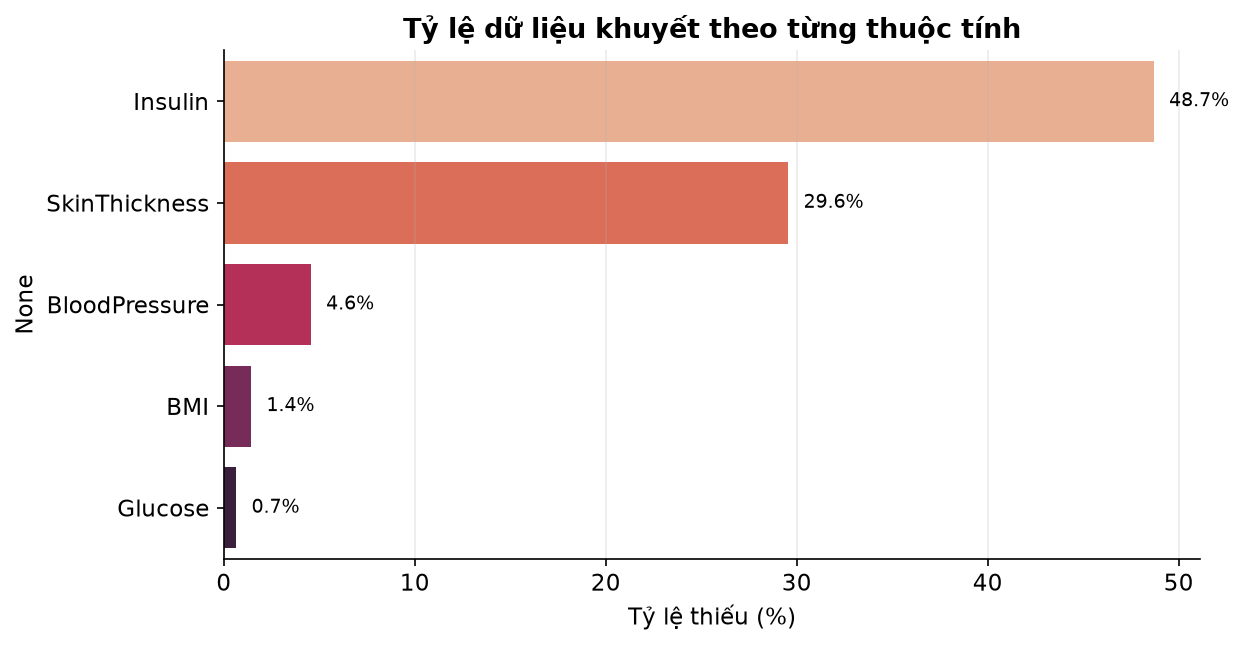
\includegraphics[width=0.78\textwidth]{dia_missing_ratio.png}
\caption[Tỷ lệ dữ liệu khuyết sau khi áp quy ước ``0 là khuyết'']%
{Tỷ lệ dữ liệu khuyết ở năm cột sinh học sau khi áp quy ước ``giá trị 0 là dữ
liệu không đo được''}
\label{fig:dia-missing}
\end{figure}

\bieudo{Biểu đồ cột ngang (horizontal bar chart), sắp xếp giảm dần theo tỷ lệ
khuyết. Trục ngang là tỷ lệ phần trăm, trục dọc là tên cột.}

\phanphoi{Phân bố cực kỳ không đều giữa các cột. Hai cột đầu chiếm gần như toàn
bộ lượng khuyết, năm cột còn lại gộp lại chưa tới $7\%$.}

\chitiet{\texttt{Insulin} khuyết $48{,}7\%$ --- gần một nửa dữ liệu.
\texttt{SkinThickness} khuyết $29{,}6\%$. Ba cột còn lại lần lượt $4{,}6\%$,
$1{,}4\%$ và $0{,}7\%$. Không cột nào vượt ngưỡng loại bỏ $80\%$ nên cả năm cột
đều được giữ lại và điền khuyết bằng trung vị.}

\begin{phathien}{Rò rỉ nhãn qua bước điền khuyết --- một sai lầm thật đã xảy ra}
\label{sec:roro}
Bản triển khai đầu tiên điền khuyết bằng \emph{trung vị theo nhóm} \texttt{Outcome}
--- tức người bệnh được điền bằng trung vị của người bệnh. Kết quả nhảy lên
Accuracy $0{,}8705$, vượt xa trần $0{,}77$--$0{,}79$ mà tài liệu công bố trên
cùng tập dữ liệu này~\cite{smith1988}. Con số đẹp bất thường ấy chính là dấu hiệu của lỗi.

Nguyên nhân: với \texttt{Insulin} khuyết $374/768$ và \texttt{SkinThickness}
khuyết $227/768$, gần một nửa dữ liệu sau khi điền đã mang dấu vết của chính
nhãn cần dự đoán. Mô hình không học quan hệ sinh học; nó đọc ngược ra nhãn từ
giá trị đã điền.

Cách sửa: đưa \texttt{SimpleImputer(strategy="median")} vào \emph{bên trong}
\texttt{Pipeline}, để \texttt{fit} chỉ nhìn thấy tập huấn luyện. Accuracy trở
về $0{,}7914$ --- thấp hơn, nhưng là con số thật. \textbf{Bài học: một kết quả
vượt trần tài liệu là lý do để đi tìm lỗi, không phải lý do để ăn mừng.}
\end{phathien}

\section{Phân tích khám phá dữ liệu}
\label{sec:eda-dia}

\subsection{Phân phối biến mục tiêu}

\begin{figure}[H]
\centering
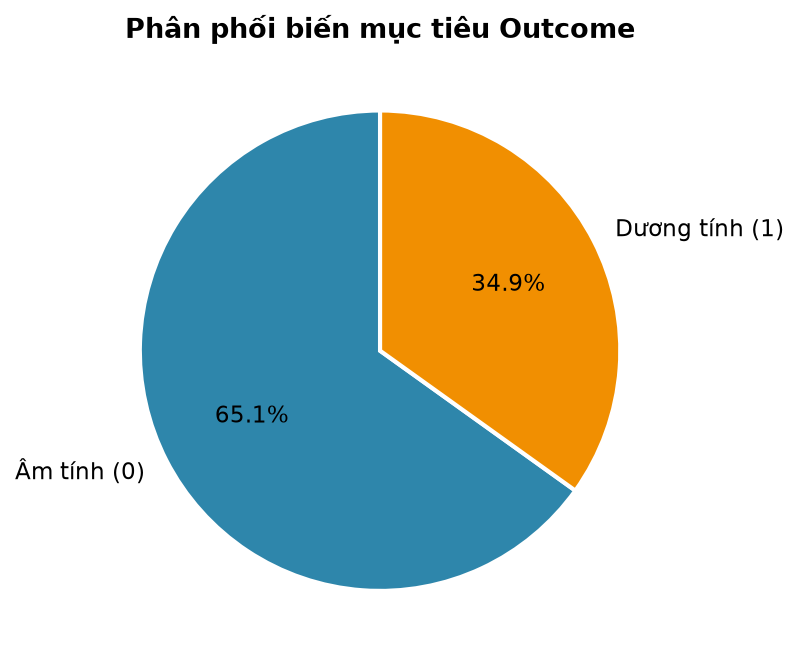
\includegraphics[width=0.56\textwidth]{dia_pie_outcome.png}
\caption[Phân phối hai lớp của biến mục tiêu \texttt{Outcome}]%
{Phân phối hai lớp của biến mục tiêu \texttt{Outcome}}
\label{fig:dia-pie}
\end{figure}

\bieudo{Biểu đồ tròn (pie chart) --- dạng phù hợp khi cần thể hiện tỷ trọng của
một số ít hạng mục trên tổng thể.}

\phanphoi{Lệch lớp ở mức trung bình, tỷ lệ xấp xỉ $2:1$ nghiêng về lớp âm tính.}

\chitiet{500 ca âm tính chiếm $65{,}1\%$ và 268 ca dương tính chiếm $34{,}9\%$.
Mức lệch này chưa tới ngưỡng ``mất cân bằng nghiêm trọng'' (thường tính từ
$10:1$) nên không cần lấy mẫu lại, nhưng đã đủ để làm Accuracy mất ý nghĩa:
một mô hình đoán bừa ``tất cả đều khoẻ'' đạt ngay $65{,}1\%$.}

\subsection{Phân phối đặc trưng quan trọng nhất}

\begin{figure}[H]
\centering
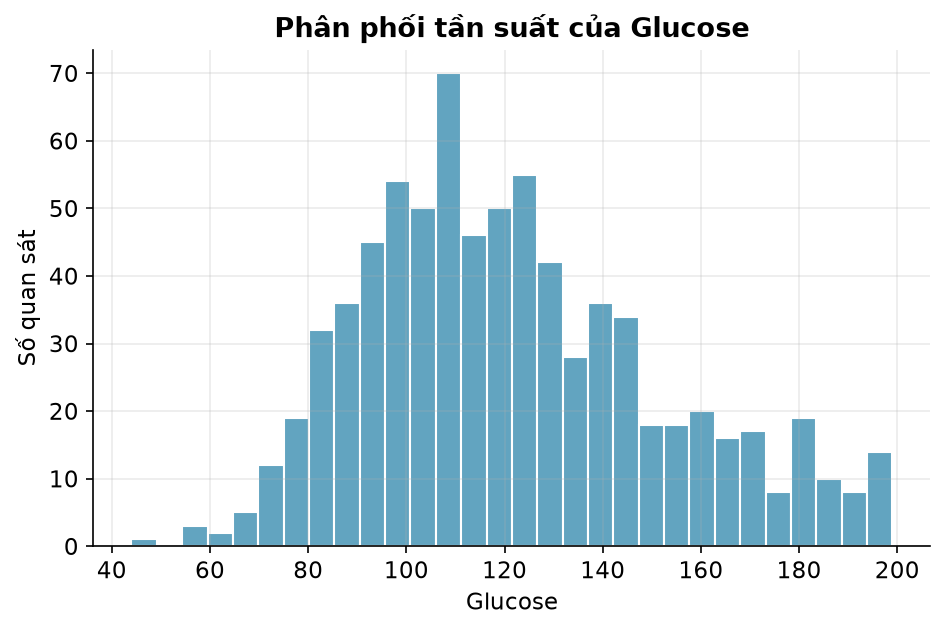
\includegraphics[width=0.78\textwidth]{dia_hist_glucose.png}
\caption[Phân phối tần suất của đặc trưng \texttt{Glucose}]%
{Phân phối tần suất của đặc trưng \texttt{Glucose}}
\label{fig:dia-hist-glucose}
\end{figure}

\bieudo{Biểu đồ tần suất (histogram). Dải giá trị liên tục được chia thành các
khoảng bằng nhau, chiều cao mỗi cột là số quan sát rơi vào khoảng đó.}

\phanphoi{Dạng gần chuẩn nhưng lệch phải nhẹ, một đỉnh duy nhất (unimodal).}

\chitiet{Khối lượng dữ liệu tập trung trong khoảng $90$--$140$ mg/dL, đỉnh tại
khoảng $105$--$115$ mg/dL với gần 70 quan sát. Đuôi trái mỏng, bắt đầu từ
khoảng $45$ mg/dL. Đuôi phải dày hơn hẳn và kéo tới $199$ mg/dL --- vùng này
tương ứng với ngưỡng chẩn đoán đái tháo đường ($\ge 200$ mg/dL sau nghiệm pháp
dung nạp), nên độ dày của đuôi phải chính là tín hiệu mà mô hình khai thác.}

\subsection{So sánh phân phối giữa hai nhóm}

\begin{figure}[H]
\centering
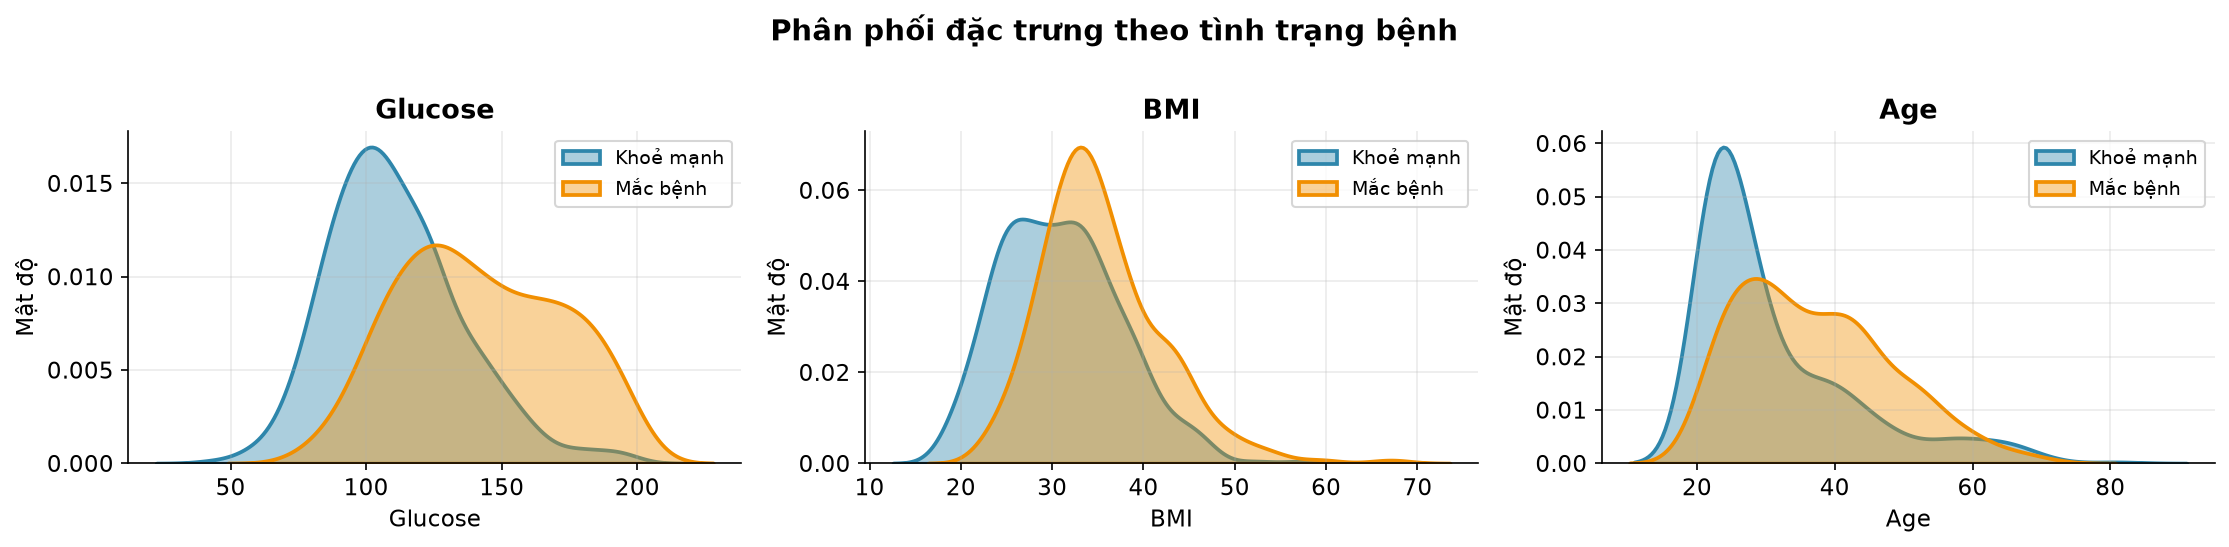
\includegraphics[width=\textwidth]{dia_kde_by_class.png}
\caption[Phân phối mật độ ba đặc trưng chính, tách theo tình trạng bệnh]%
{Ước lượng mật độ hạt nhân (KDE) của \texttt{Glucose}, \texttt{BMI} và
\texttt{Age}, tách theo tình trạng bệnh}
\label{fig:dia-kde-class}
\end{figure}

\bieudo{Ba biểu đồ mật độ hạt nhân chồng lớp (overlaid KDE). Khác biểu đồ tần
suất, KDE dùng đường cong liên tục nên hình dáng phân phối không phụ thuộc vào
cách chọn độ rộng khoảng. Hai màu là hai nhóm của biến mục tiêu.}

\phanphoi{Cả ba cặp đường cong đều lệch nhau theo cùng một hướng --- nhóm mắc
bệnh dịch sang phải --- nhưng \emph{mức độ} tách rời rất khác nhau.}

\chitiet{\texttt{Glucose} tách rõ nhất: đỉnh nhóm khoẻ ở khoảng $105$ mg/dL,
đỉnh nhóm bệnh ở khoảng $135$--$145$ mg/dL, và phần chồng lấn tuy còn lớn nhưng
hai đỉnh đã tách hẳn. \texttt{BMI} tách vừa phải, hai đỉnh chỉ cách nhau vài đơn
vị quanh mốc $30$--$35$ kg/m$^2$. \texttt{Age} tách yếu nhất: nhóm khoẻ có một
đỉnh nhọn ở khoảng $22$--$25$ tuổi, nhóm bệnh phân bố thoải và rộng hơn nhưng
phần chồng lấn chiếm gần trọn vùng dữ liệu.}

\nhanxet{Thứ tự tách rời ở đây --- \texttt{Glucose} $>$ \texttt{BMI} $>$
\texttt{Age} --- báo trước đúng thứ tự tương quan với nhãn ở
Bảng~\ref{tab:corr-dia} và đúng thứ tự mức quan trọng đặc trưng ở
Hình~\ref{fig:dia-importance}. Ba phương pháp độc lập cùng chỉ về một kết luận
là bằng chứng mạnh hơn bất kỳ phương pháp nào đứng riêng.}

\subsection{Giá trị ngoại lai}

\begin{figure}[H]
\centering
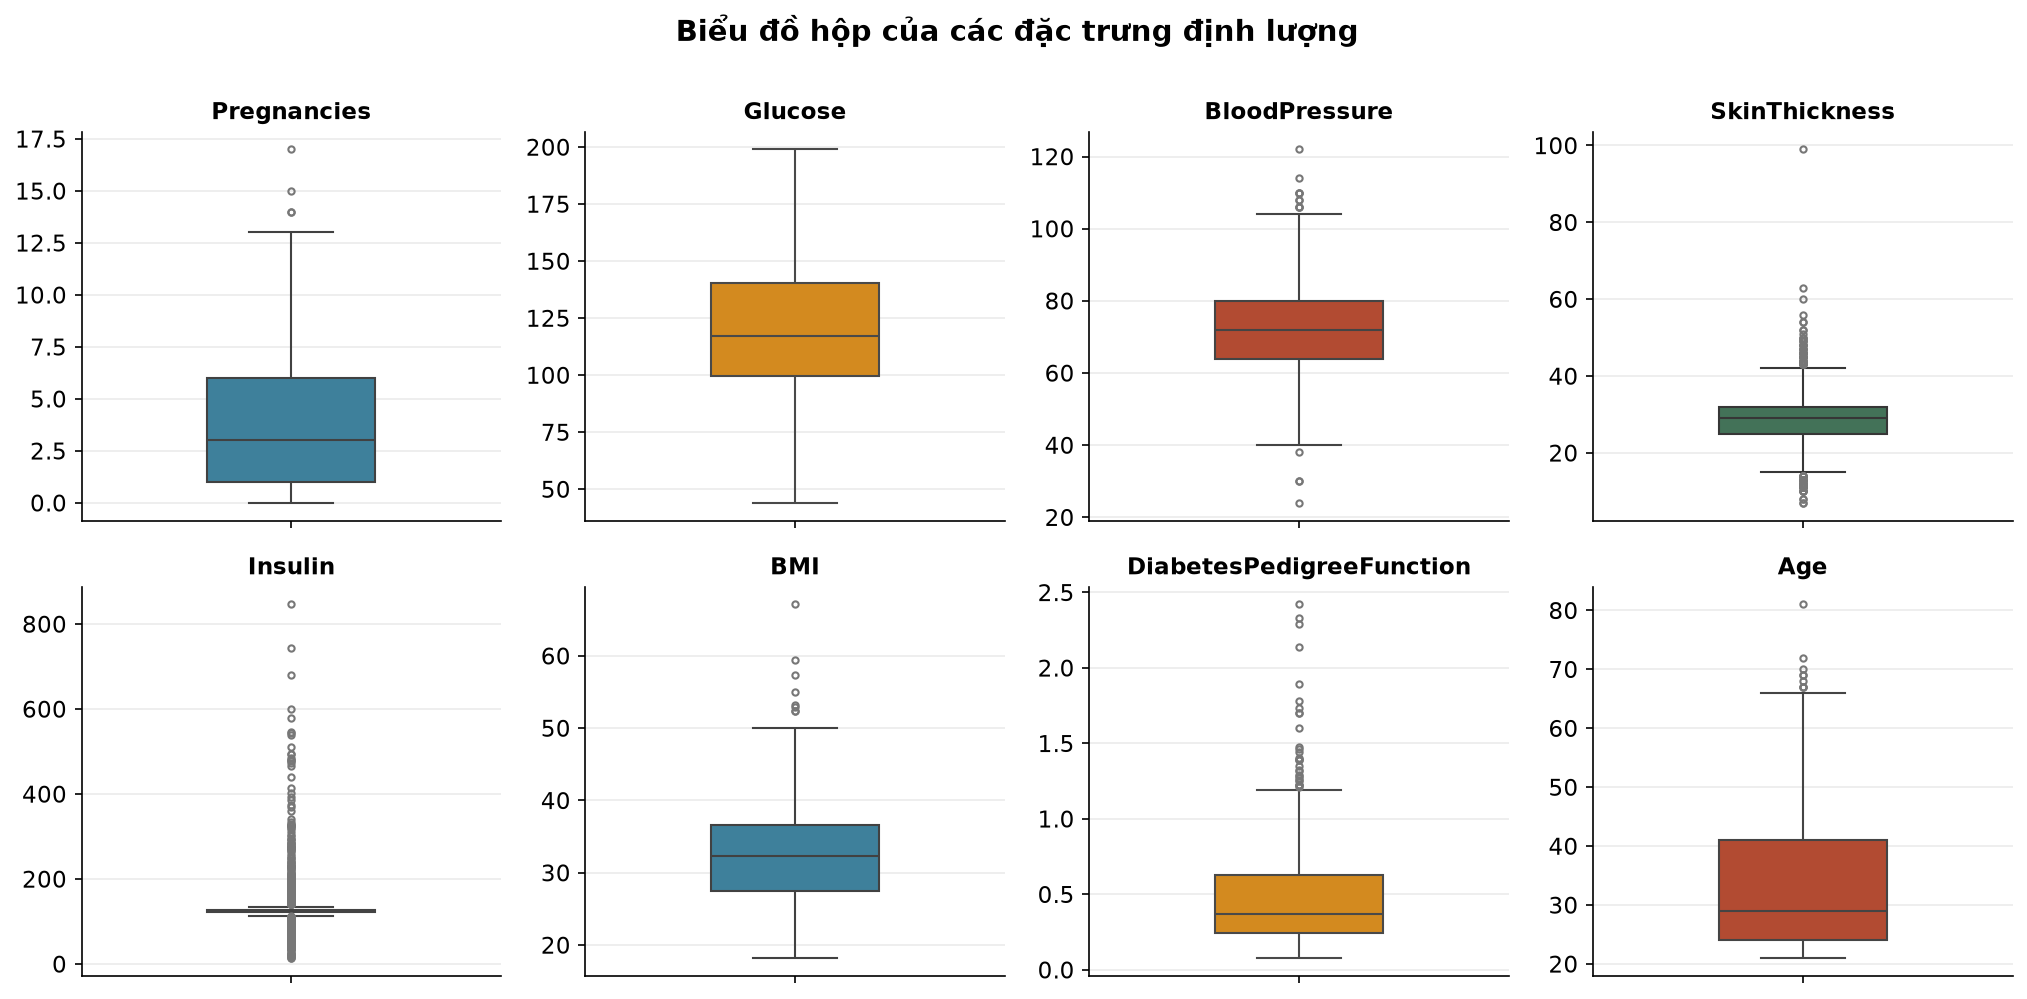
\includegraphics[width=\textwidth]{dia_box_grid.png}
\caption[Biểu đồ hộp của tám đặc trưng định lượng]%
{Biểu đồ hộp của tám đặc trưng định lượng}
\label{fig:dia-box}
\end{figure}

\bieudo{Lưới tám biểu đồ hộp (boxplot). Hộp bao phủ khoảng tứ phân vị Q1--Q3,
đường giữa là trung vị, râu kéo dài tối đa $1{,}5\times$IQR, mọi điểm ngoài râu
được đánh dấu là ngoại lai.}

\phanphoi{Ba nhóm khác hẳn nhau. Nhóm gọn gàng: \texttt{Glucose},
\texttt{BloodPressure}, \texttt{BMI} --- hộp cân đối, ít điểm ngoài râu. Nhóm
lệch phải mạnh: \texttt{Insulin}, \texttt{DiabetesPedigreeFunction},
\texttt{Age}. Nhóm đặc biệt: \texttt{SkinThickness}, có hộp rất hẹp.}

\chitiet{\texttt{Insulin} có hộp nén sát đáy với một dải điểm ngoại lai dày đặc
kéo lên tới hơn $800$ $\mu$U/mL --- hệ quả trực tiếp của việc $48{,}7\%$ giá trị
được điền bằng cùng một con số trung vị, khiến hộp co lại quanh giá trị ấy.
\texttt{SkinThickness} cũng cho hình dáng tương tự vì lý do y hệt.
\texttt{Age} có hộp trải từ khoảng $25$ tới $41$ tuổi với đuôi trên kéo tới
$81$. \texttt{Pregnancies} là biến đếm nên hình dáng bậc thang, tối đa $17$ lần.}

\nhanxet{Không giá trị ngoại lai nào bị loại bỏ. Với dữ liệu y sinh, một chỉ số
cực đoan thường là \emph{ca bệnh nặng} --- đúng nhóm mà hệ thống sàng lọc cần
phát hiện nhất. Loại bỏ chúng là loại bỏ tín hiệu, không phải loại bỏ nhiễu.}

\section{Thiết kế đặc trưng}
\label{sec:dactrung-dia}

Bốn đặc trưng phái sinh được xây từ tri thức y học, không phải từ tìm kiếm mù:

\begin{table}[H]
\centering
\caption{Bốn đặc trưng thiết kế và căn cứ y học}
\label{tab:engineered-dia}
\small
\begin{tabularx}{\textwidth}{@{}L{3.2cm}L{4.0cm}X@{}}
\toprule
\textbf{Đặc trưng} & \textbf{Công thức} & \textbf{Căn cứ} \\
\midrule
\texttt{Glucose\_BMI\_Risk} & $\texttt{Glucose}\times\texttt{BMI}$ &
Tăng đường huyết đi kèm béo phì có rủi ro cao hơn tổng rủi ro của hai yếu tố
riêng lẻ --- một tương tác mà mô hình tuyến tính không tự tạo ra được \\
\addlinespace
\texttt{Glucose\_Level} & Rời rạc hoá theo ngưỡng lâm sàng &
Ba mức: bình thường, tiền đái tháo đường, đái tháo đường \\
\addlinespace
\texttt{BMI\_Class} & Rời rạc hoá theo phân loại WHO &
Bốn mức: gầy, bình thường, thừa cân, béo phì \\
\addlinespace
\texttt{Age\_Group} & Rời rạc hoá theo nhóm tuổi &
Rủi ro tăng không tuyến tính theo tuổi \\
\bottomrule
\end{tabularx}
\end{table}

\section{Ma trận tương quan và sàng lọc đặc trưng}
\label{sec:corr-dia}

\begin{figure}[H]
\centering
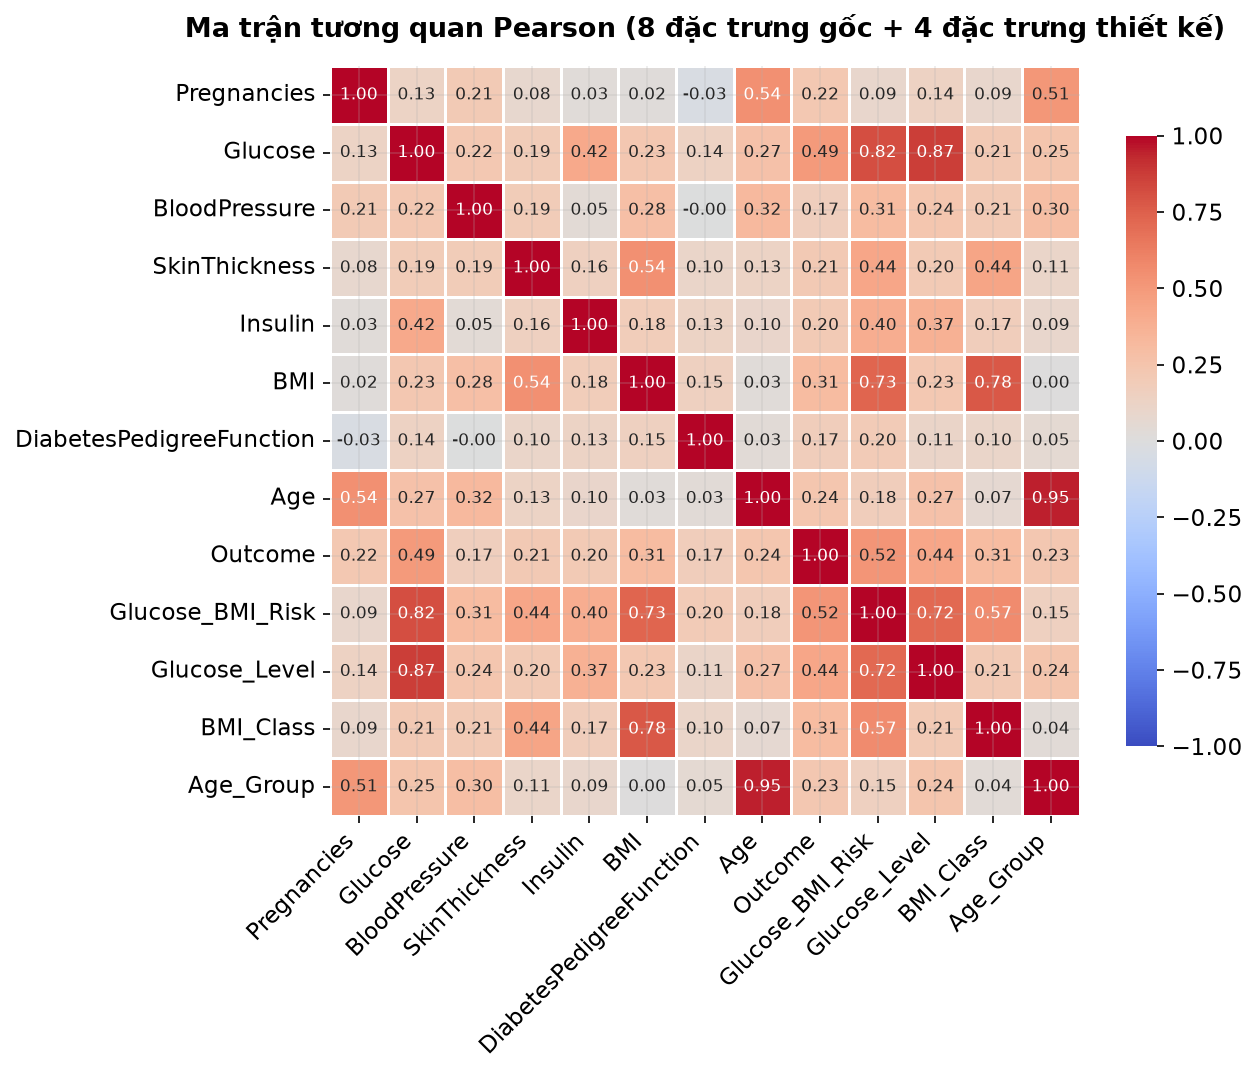
\includegraphics[width=\textwidth]{dia_corr_heatmap.png}
\caption[Ma trận tương quan Pearson của 8 đặc trưng gốc và 4 đặc trưng thiết kế]%
{Ma trận tương quan Pearson --- 8 đặc trưng gốc, 4 đặc trưng thiết kế và biến
mục tiêu}
\label{fig:dia-corr}
\end{figure}

\bieudo{Bản đồ nhiệt (heatmap) đối xứng. Màu đỏ là tương quan dương, màu xanh là
tương quan âm, độ đậm tỷ lệ với độ lớn hệ số.}

\phanphoi{Toàn bộ ma trận nghiêng về phía đỏ nhạt --- không có cặp nào tương
quan âm đáng kể. Ba cụm đậm nổi lên rõ, tất cả đều là cặp gốc -- phái sinh.}

\chitiet{Ba cặp đậm nhất đều do định nghĩa mà có:
\texttt{Glucose}--\texttt{Glucose\_Level} $=0{,}87$,
\texttt{Glucose}--\texttt{Glucose\_BMI\_Risk} $=0{,}82$,
\texttt{Age}--\texttt{Age\_Group} $=0{,}95$ và
\texttt{BMI}--\texttt{BMI\_Class} $=0{,}78$. Với biến mục tiêu, cột
\texttt{Outcome} có màu nhạt hơn hẳn: hệ số cao nhất chỉ là $0{,}52$.}

\begin{table}[H]
\centering
\caption{Tương quan Pearson với biến mục tiêu \texttt{Outcome}, sắp giảm dần}
\label{tab:corr-dia}
\small
\begin{tabular}{@{}lrlr@{}}
\toprule
\textbf{Đặc trưng} & \textbf{$\rho$} & \textbf{Đặc trưng} & \textbf{$\rho$} \\
\midrule
\texttt{Glucose\_BMI\_Risk} & \textbf{0{,}5199} & \texttt{Age\_Group}     & 0{,}2322 \\
\texttt{Glucose}            & 0{,}4928 & \texttt{Pregnancies}    & 0{,}2219 \\
\texttt{Glucose\_Level}     & 0{,}4356 & \texttt{SkinThickness}  & 0{,}2149 \\
\texttt{BMI}                & 0{,}3120 & \texttt{Insulin}        & 0{,}2038 \\
\texttt{BMI\_Class}         & 0{,}3098 & \texttt{DiabetesPedigreeFunction} & 0{,}1738 \\
\texttt{Age}                & 0{,}2384 & \texttt{BloodPressure}  & 0{,}1657 \\
\bottomrule
\end{tabular}
\end{table}

\nhanxet{Đặc trưng thiết kế \texttt{Glucose\_BMI\_Risk} tương quan với nhãn
\emph{mạnh hơn} cả \texttt{Glucose} gốc ($0{,}5199$ so với $0{,}4928$) ---
bằng chứng định lượng cho thấy tri thức y học đưa vào đúng chỗ có giá trị. Ngưỡng
sàng lọc $|\rho|\ge0{,}20$ giữ lại năm đặc trưng gốc: \texttt{Glucose},
\texttt{SkinThickness}, \texttt{Insulin}, \texttt{BMI}, \texttt{Age}.

Cần nói rõ giới hạn: hệ số Pearson chỉ đo quan hệ \textbf{tuyến tính}. Giá trị
gần $0$ không loại trừ quan hệ phi tuyến mạnh, nên bảng này được dùng để
\emph{xếp hạng} chứ không dùng làm căn cứ duy nhất để loại đặc trưng --- mọi mô
hình trong chương vẫn nhận đủ 12 cột.}

\section{Chia dữ liệu và mô hình cơ sở}

Áp dụng giao thức ba tập ở Mục~\ref{sec:giaothuc}, có phân tầng theo nhãn để
giữ nguyên tỷ lệ $65/35$ trong cả ba tập:

\begin{table}[H]
\centering
\caption{Kích thước ba tập dữ liệu và kết quả mô hình cơ sở}
\label{tab:split-dia}
\small
\begin{tabular}{@{}lrr@{\hspace{1.5cm}}lr@{}}
\toprule
\textbf{Tập} & \textbf{Số ca} & \textbf{Tỷ lệ} & \textbf{Mô hình cơ sở} & \textbf{Giá trị} \\
\midrule
Huấn luyện & 552 & 71{,}9\% & Accuracy  & 0{,}6547 \\
Kiểm tra   & 139 & 18{,}1\% & Precision & 0{,}0000 \\
Ngoại kiểm &  77 & 10{,}0\% & Recall    & \textbf{0{,}0000} \\
\textbf{Tổng} & \textbf{768} & \textbf{100\%} & $F_1$ & 0{,}0000 \\
\bottomrule
\end{tabular}
\end{table}

\begin{phathien}{Vì sao Accuracy $0{,}6547$ là một con số nguy hiểm}
Mô hình cơ sở luôn đoán ``khoẻ mạnh''. Nó đúng $65{,}47\%$ số lần --- nghe không
tệ. Nhưng Recall bằng $0$: nó \textbf{bỏ sót toàn bộ 48 người bệnh} trong tập
kiểm tra. Một hệ thống sàng lọc như vậy vô dụng hoàn toàn, dù chỉ số Accuracy
của nó cao hơn cả XGBoost ($0{,}7194$)~\dots{} không, thực ra thấp hơn --- nhưng
khoảng cách chỉ là $6$ điểm phần trăm, đủ nhỏ để một báo cáo chỉ nhìn Accuracy
kết luận sai rằng ``mô hình học được chẳng hơn bao nhiêu''. $F_1$ nói đúng sự
thật: $0{,}0000$ so với $0{,}5895$.
\end{phathien}

\section{Thực nghiệm 1 --- Đối đầu năm mô hình}
\label{sec:tn1-dia}

\textbf{Câu hỏi.} Trong năm nguyên lý học khác nhau, nguyên lý nào hợp với cấu
trúc của dữ liệu y sinh này?

\textbf{Thiết kế.} Năm mô hình nhận \emph{cùng} một biểu diễn, \emph{cùng} một
phép chia dữ liệu, \emph{cùng} một hạt giống ngẫu nhiên. Chỉ thuật toán thay đổi.

\begin{table}[H]
\centering
\caption{Kết quả năm mô hình phân lớp trên tập kiểm tra, sắp theo $F_1$}
\label{tab:ketqua-dia}
\small
\begin{tabular}{@{}lrrrrr@{}}
\toprule
\textbf{Mô hình} & \textbf{Accuracy} & \textbf{Precision} & \textbf{Recall} & \textbf{$F_1$} & \textbf{ROC-AUC} \\
\midrule
Mô hình cơ sở        & 0{,}6547 & 0{,}0000 & 0{,}0000 & 0{,}0000 & --- \\
\midrule
K-Nearest Neighbors  & 0{,}7842 & 0{,}6957 & \textbf{0{,}6667} & \textbf{0{,}6809} & 0{,}8462 \\
Logistic Regression  & \textbf{0{,}7914} & \textbf{0{,}7436} & 0{,}6042 & 0{,}6667 & \textbf{0{,}8709} \\
XGBoost              & 0{,}7194 & 0{,}5957 & 0{,}5833 & 0{,}5895 & 0{,}7905 \\
Random Forest        & 0{,}7194 & 0{,}6154 & 0{,}5000 & 0{,}5517 & 0{,}8191 \\
Decision Tree        & 0{,}7266 & 0{,}6786 & 0{,}3958 & 0{,}5000 & 0{,}7446 \\
\bottomrule
\end{tabular}
\end{table}

\begin{figure}[H]
\centering
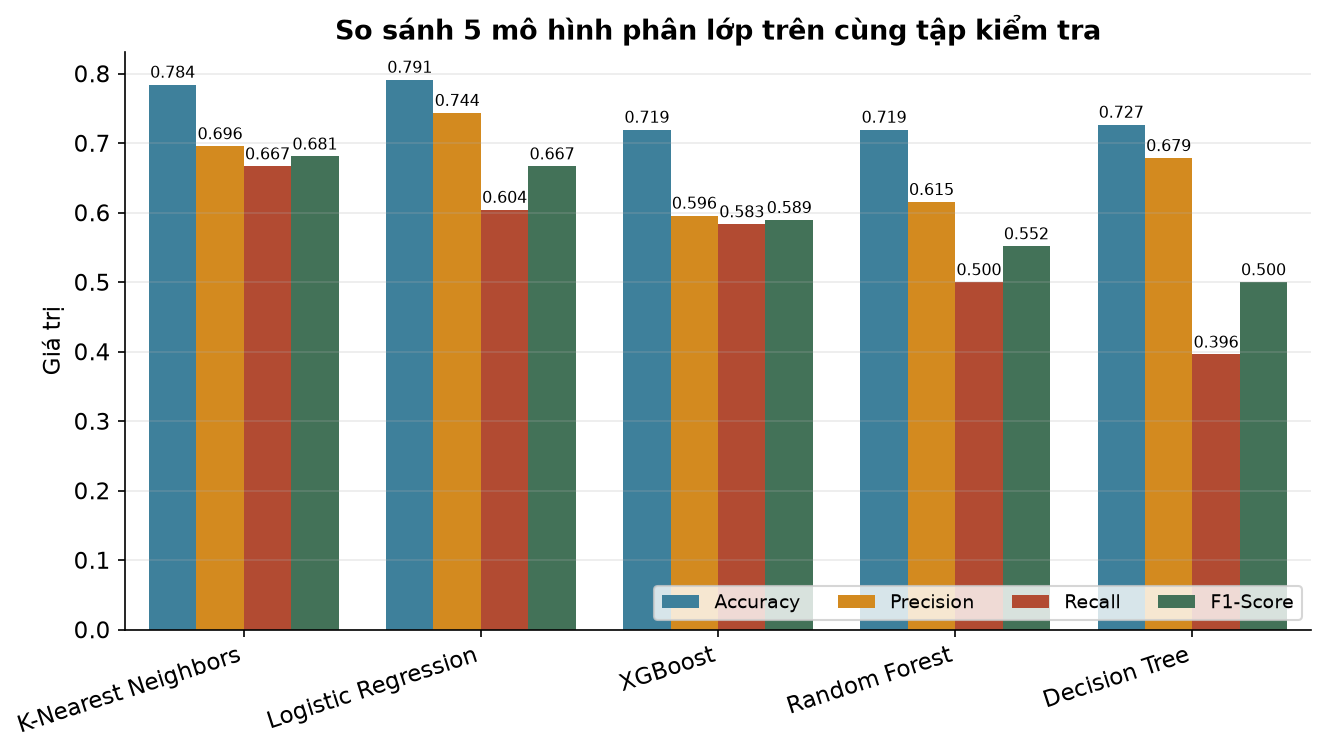
\includegraphics[width=\textwidth]{dia_model_comparison.png}
\caption[So sánh năm mô hình phân lớp trên bốn độ đo]%
{So sánh năm mô hình phân lớp trên cùng tập kiểm tra, bốn độ đo}
\label{fig:dia-comparison}
\end{figure}

\bieudo{Biểu đồ cột nhóm (grouped bar chart). Mỗi nhóm là một mô hình, bốn cột
trong nhóm là bốn độ đo.}

\nhanxet{Ba điều đáng chú ý.

\textbf{(1) Cả năm mô hình đều vượt mô hình cơ sở} ở $F_1$ và Recall --- việc
học mang lại giá trị thật, không phải chỉ là trang trí.

\textbf{(2) Hai mô hình đơn giản nhất thắng.} K-Nearest Neighbors và Logistic
Regression đứng đầu, còn hai mô hình tổ hợp phức tạp hơn hẳn --- Random Forest
và XGBoost --- lại xếp sau. Với 552 mẫu huấn luyện và 12 đặc trưng, các mô hình
có phương sai cao không đủ dữ liệu để phát huy; đây là minh hoạ sách giáo khoa
cho đánh đổi độ chệch -- phương sai.

\textbf{(3) Không có mô hình nào thắng trên mọi độ đo.} Logistic Regression dẫn
đầu Accuracy, Precision và ROC-AUC; K-Nearest Neighbors dẫn đầu Recall và $F_1$.
Với mục tiêu sàng lọc, KNN là lựa chọn đúng --- nó bỏ sót ít người bệnh hơn.}

\subsection{Đường cong ROC --- khả năng xếp hạng độc lập với ngưỡng}

\begin{figure}[H]
\centering
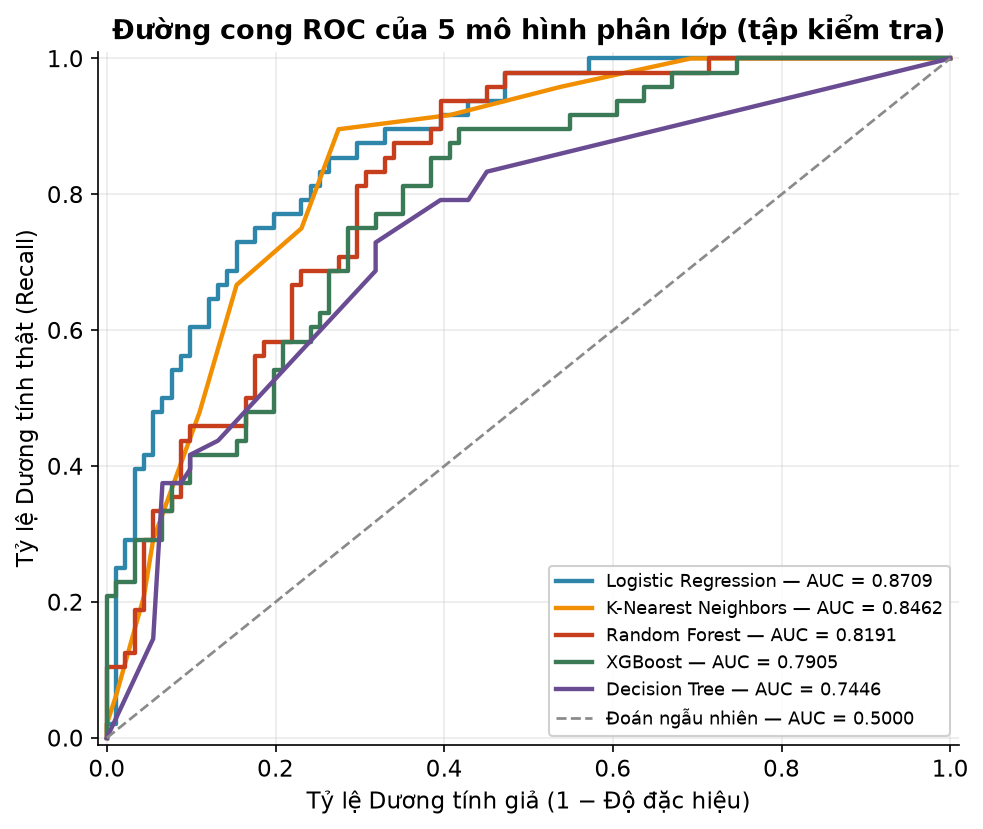
\includegraphics[width=0.72\textwidth]{dia_roc_curves.png}
\caption[Đường cong ROC của năm mô hình phân lớp]%
{Đường cong ROC của năm mô hình phân lớp trên tập kiểm tra, kèm diện tích dưới
đường cong (AUC)}
\label{fig:dia-roc}
\end{figure}

\bieudo{Đường cong ROC (Receiver Operating Characteristic). Trục ngang là tỷ lệ
Dương tính giả, trục dọc là Recall; mỗi điểm trên đường cong ứng với một ngưỡng
quyết định. Đường chéo nét đứt là mốc đoán ngẫu nhiên.}

\phanphoi{Cả năm đường đều nằm hẳn phía trên đường chéo --- mọi mô hình đều xếp
hạng tốt hơn ngẫu nhiên. Chúng bó lại thành một chùm hẹp ở góc trên bên trái rồi
toả ra ở vùng giữa.}

\chitiet{Logistic Regression dẫn đầu với AUC $=0{,}8709$, bám sát là K-Nearest
Neighbors $0{,}8462$ và Random Forest $0{,}8191$. XGBoost đạt $0{,}7905$, còn
Decision Tree tụt hẳn xuống $0{,}7446$ --- đường cong của nó có dạng gãy khúc
thành vài đoạn thẳng dài thay vì cong mượt.}

\begin{phathien}{Thứ tự trên ROC không trùng thứ tự trên $F_1$ --- và đó không phải mâu thuẫn}
Logistic Regression dẫn đầu AUC nhưng chỉ đứng thứ hai về $F_1$; K-Nearest
Neighbors thì ngược lại. Hai độ đo trả lời hai câu hỏi khác nhau:

\begin{itemize}
  \item \textbf{AUC} hỏi \emph{mô hình có xếp người bệnh lên trên người khoẻ
        không}, xét trên mọi ngưỡng cùng lúc.
  \item \textbf{$F_1$} hỏi \emph{tại ngưỡng $0{,}50$, mô hình cắt có tốt không}.
\end{itemize}

Một mô hình xếp hạng giỏi mà bị cắt sai chỗ vẫn cho $F_1$ thấp. Đó chính là khe
hở mà Thực nghiệm~2 khai thác ở Mục~\ref{sec:tn2-dia}: giữ nguyên mô hình, chỉ
đổi điểm cắt, và $F_1$ tăng trong khi AUC không đổi một chút nào.

Dạng gãy khúc của đường cong Decision Tree cũng là một tín hiệu chẩn đoán: cây
sâu 6 tầng chỉ trả về vài giá trị xác suất rời rạc, nên đường cong chỉ có vài
điểm gấp. Chi tiết này sẽ quay lại ở Mục~\ref{sec:tn2-dia}.
\end{phathien}

\subsection{Lưới ma trận nhầm lẫn --- sai theo kiểu gì}

\begin{figure}[H]
\centering
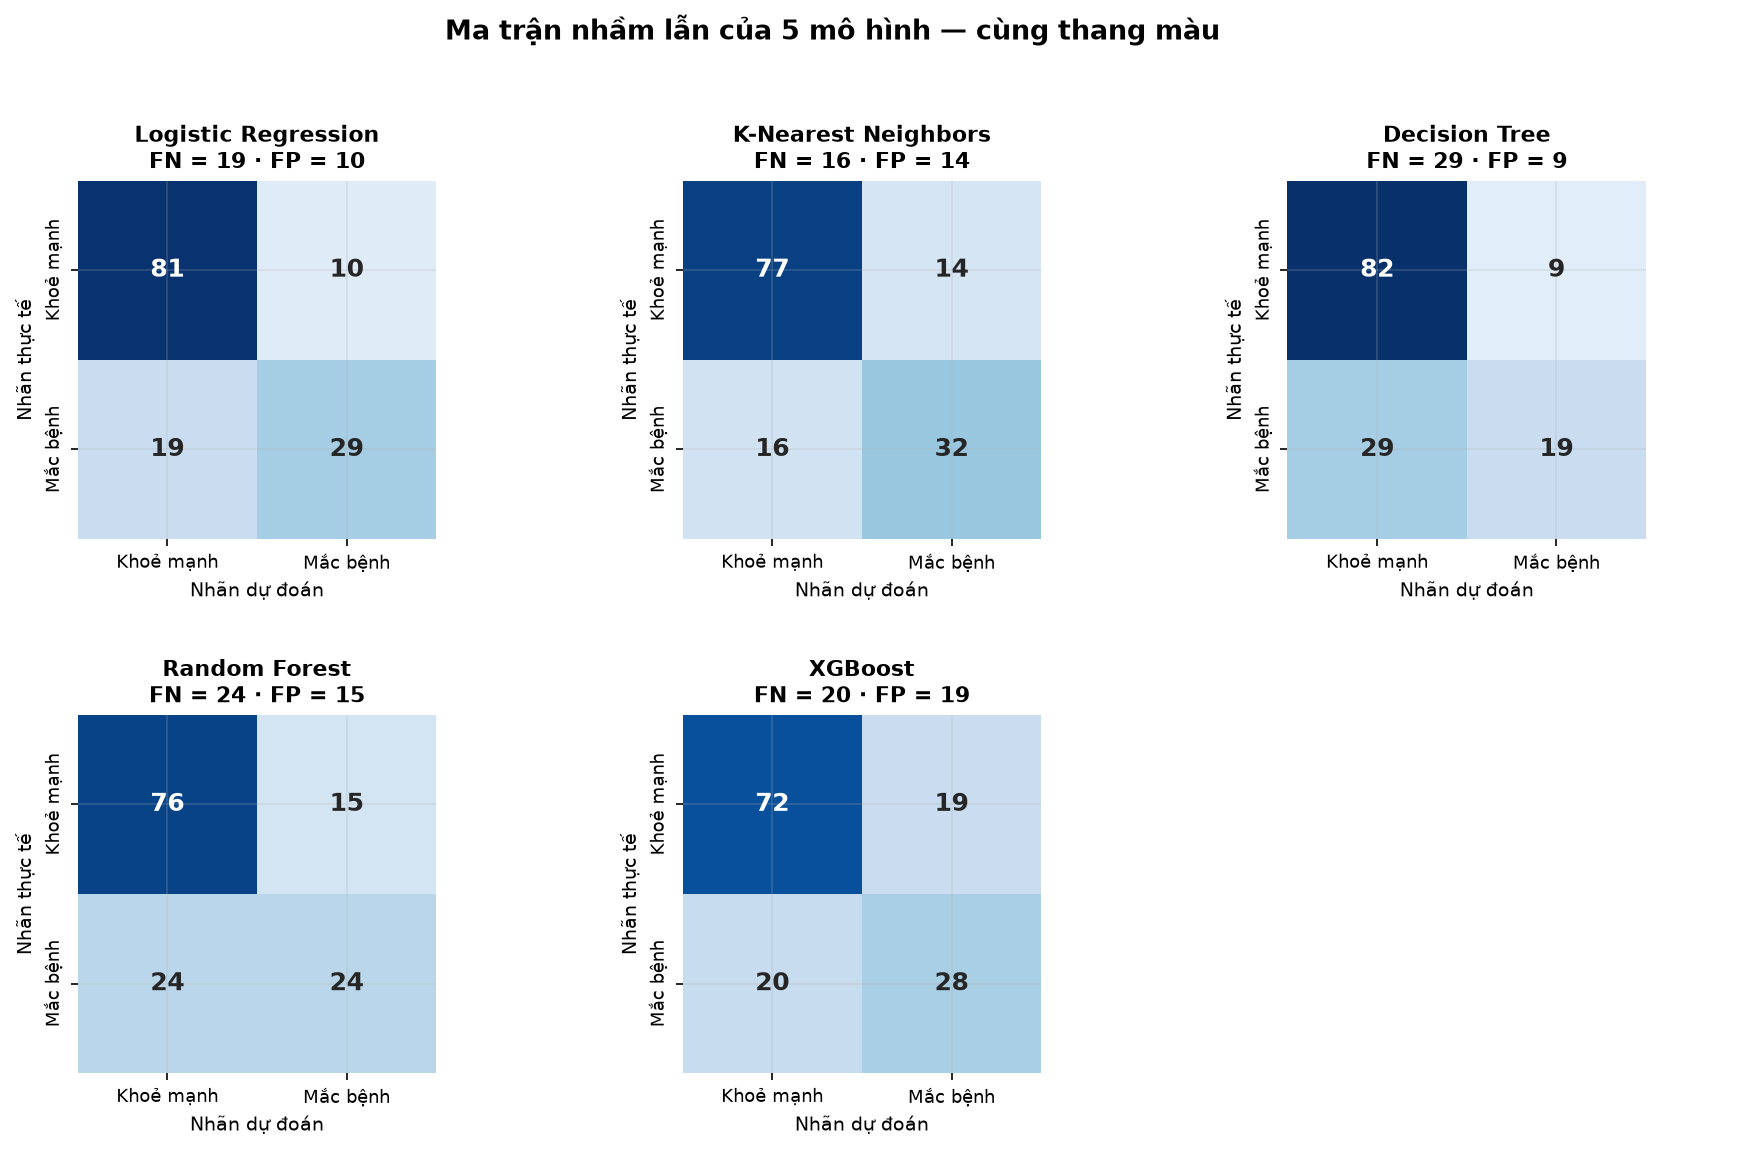
\includegraphics[width=\textwidth]{dia_confusion_grid.png}
\caption[Ma trận nhầm lẫn của năm mô hình trên cùng một thang màu]%
{Ma trận nhầm lẫn của năm mô hình phân lớp, dùng chung một thang màu để so sánh
trực tiếp}
\label{fig:dia-cm-grid}
\end{figure}

\bieudo{Lưới bản đồ nhiệt (heatmap grid), mỗi ô là một ma trận nhầm lẫn $2\times2$.
Mọi ô dùng chung một thang màu nên độ đậm so sánh được trực tiếp giữa các mô
hình. Số FN và FP ghi ngay dưới tên mô hình.}

\phanphoi{Cấu trúc giống nhau ở cả năm ô: ô góc trên trái (TN) luôn đậm nhất,
ba ô còn lại nhạt hơn hẳn --- hệ quả của việc lớp âm tính đông gần gấp đôi.
Điều thay đổi giữa các mô hình là \emph{tỷ lệ} giữa hai ô sai.}

\chitiet{K-Nearest Neighbors có FN thấp nhất ($16$) --- nó bỏ sót ít người bệnh
nhất. Decision Tree có FN cao nhất ($29$), gần gấp đôi, dù Accuracy của nó
($0{,}7266$) còn cao hơn XGBoost ($0{,}7194$). Ở chiều ngược lại, Decision Tree
lại có FP thấp nhất ($9$): nó thận trọng tới mức hiếm khi báo động, và cái giá
phải trả là bỏ sót.}

\nhanxet{Đây là bằng chứng trực quan cho luận điểm ở Mục~\ref{sec:baseline}:
\textbf{Accuracy che mất đúng loại sai lầm đắt nhất}. Hai mô hình chênh nhau
$0{,}7$ điểm phần trăm Accuracy nhưng chênh nhau $13$ người bệnh bị bỏ sót trên
tổng số $48$ --- tức hơn một phần tư số ca cần tìm.}

\section{Thực nghiệm 2 --- Siêu tham số và ngưỡng quyết định}
\label{sec:tn2-dia}

\subsection{Khảo sát số láng giềng $k$}

\begin{figure}[H]
\centering
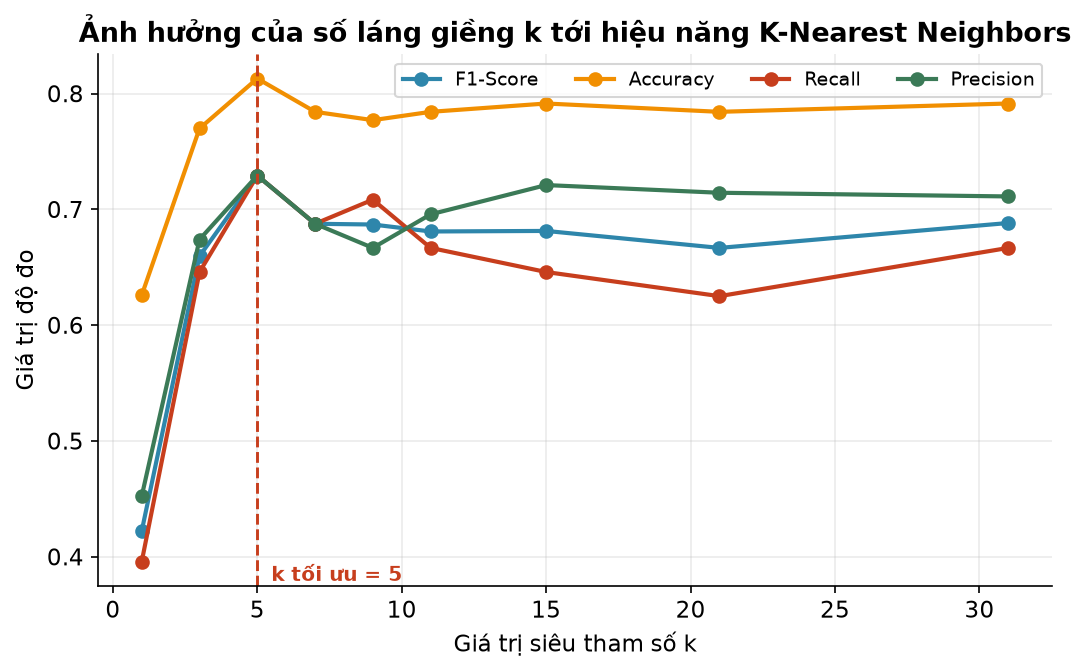
\includegraphics[width=0.88\textwidth]{dia_knn_k_sweep.png}
\caption[Ảnh hưởng của số láng giềng $k$ tới bốn độ đo]%
{Ảnh hưởng của số láng giềng $k$ tới bốn độ đo của K-Nearest Neighbors}
\label{fig:dia-k-sweep}
\end{figure}

\bieudo{Biểu đồ đường đa tuyến (multi-line plot). Trục ngang là giá trị $k$,
mỗi đường là một độ đo.}

\phanphoi{Dạng chữ U ngược đúng như lý thuyết đánh đổi độ chệch -- phương sai
dự báo, với một đỉnh rõ ràng ở đầu dải và một vùng bằng phẳng kéo dài về sau.}

\chitiet{Tại $k=1$, cả bốn độ đo đều thấp nhất ($F_1=0{,}4222$) --- mô hình học
thuộc từng điểm huấn luyện, phương sai cực đại. $F_1$ tăng vọt lên $0{,}6596$ ở
$k=3$ rồi đạt đỉnh $0{,}7292$ tại $k=5$. Từ $k=7$ trở đi đường cong đi ngang
trong dải $0{,}6667$--$0{,}6882$ mà không sụt hẳn.}

\begin{table}[H]
\centering
\caption{Khảo sát số láng giềng $k$ --- kết quả đầy đủ}
\label{tab:k-sweep}
\small
\begin{tabular}{@{}rrrrr@{}}
\toprule
\textbf{$k$} & \textbf{Accuracy} & \textbf{Precision} & \textbf{Recall} & \textbf{$F_1$} \\
\midrule
1  & 0{,}6259 & 0{,}4524 & 0{,}3958 & 0{,}4222 \\
3  & 0{,}7698 & 0{,}6739 & 0{,}6458 & 0{,}6596 \\
\textbf{5}  & \textbf{0{,}8129} & \textbf{0{,}7292} & \textbf{0{,}7292} & \textbf{0{,}7292} \\
7  & 0{,}7842 & 0{,}6875 & 0{,}6875 & 0{,}6875 \\
9  & 0{,}7770 & 0{,}6667 & 0{,}7083 & 0{,}6869 \\
11 & 0{,}7842 & 0{,}6957 & 0{,}6667 & 0{,}6809 \\
15 & 0{,}7914 & 0{,}7209 & 0{,}6458 & 0{,}6813 \\
21 & 0{,}7842 & 0{,}7143 & 0{,}6250 & 0{,}6667 \\
31 & 0{,}7914 & 0{,}7111 & 0{,}6667 & 0{,}6882 \\
\bottomrule
\end{tabular}
\end{table}

\nhanxet{Giá trị $k=11$ dùng trong danh mục mô hình ở Thực nghiệm~1 là quy tắc
kinh nghiệm $k\approx\sqrt{n}$; khảo sát cho thấy $k=5$ tốt hơn ($F_1$ $0{,}7292$
so với $0{,}6809$). Chênh lệch $0{,}048$ $F_1$ tương ứng khoảng 3 ca trên 139 ---
nằm trong biên độ nhiễu lấy mẫu của một tập kiểm tra cỡ này, nên đây là một cải
thiện \emph{có hướng} chứ chưa phải một khẳng định chắc chắn.}

\subsection{Quét ngưỡng quyết định}

Đây là thực nghiệm quan trọng nhất của cả chương, vì nó thay đổi hệ thống mà
\emph{không} đụng tới mô hình.

\begin{figure}[H]
\centering
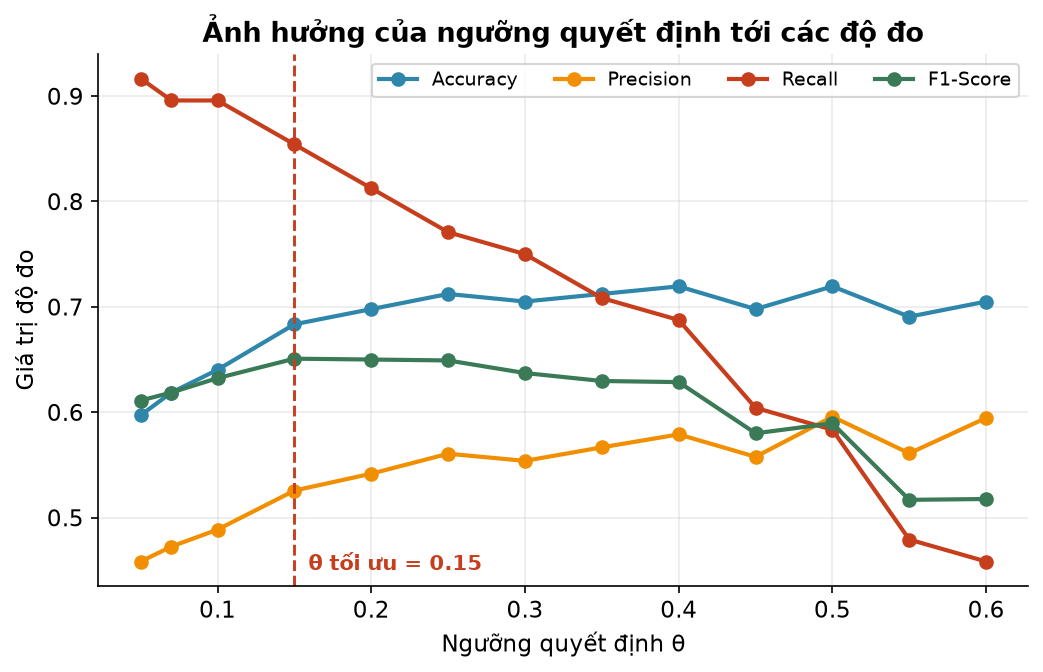
\includegraphics[width=\textwidth]{dia_threshold_curve.png}
\caption[Ảnh hưởng của ngưỡng quyết định $\theta$ tới bốn độ đo]%
{Ảnh hưởng của ngưỡng quyết định $\theta$ tới bốn độ đo, mô hình XGBoost}
\label{fig:dia-threshold}
\end{figure}

\bieudo{Biểu đồ đường đa tuyến. Trục ngang là ngưỡng $\theta$ quét từ $0{,}60$
xuống $0{,}05$; đường nét đứt dọc đánh dấu ngưỡng tối ưu theo $F_1$.}

\phanphoi{Hai đường chính chạy ngược chiều nhau và cắt nhau --- dấu hiệu kinh
điển của một đánh đổi. Hai đường còn lại biến thiên nhẹ.}

\chitiet{Recall tăng đơn điệu khi $\theta$ giảm: từ $0{,}4583$ tại
$\theta=0{,}60$ lên $0{,}9167$ tại $\theta=0{,}05$. Precision đi ngược lại, từ
$0{,}5946$ xuống $0{,}4583$. Hai đường cắt nhau quanh $\theta=0{,}50$. $F_1$ ---
trung bình điều hoà của hai đường ấy --- đạt đỉnh $0{,}6508$ tại
$\theta=0{,}15$. Accuracy gần như đi ngang trong dải $0{,}60$--$0{,}72$ suốt cả
quá trình, một lần nữa cho thấy nó không nhạy với điều đang thay đổi.}

\begin{table}[H]
\centering
\caption{Quét ngưỡng quyết định --- bốn ô ma trận nhầm lẫn tại mỗi ngưỡng}
\label{tab:threshold-dia}
\small
\begin{tabular}{@{}rrrrrrrrr@{}}
\toprule
\textbf{$\theta$} & \textbf{Accuracy} & \textbf{Precision} & \textbf{Recall} & \textbf{$F_1$} & \textbf{TP} & \textbf{FN} & \textbf{FP} & \textbf{TN} \\
\midrule
0{,}60 & 0{,}7050 & 0{,}5946 & 0{,}4583 & 0{,}5176 & 22 & 26 & 15 & 76 \\
0{,}50 & 0{,}7194 & 0{,}5957 & 0{,}5833 & 0{,}5895 & 28 & 20 & 19 & 72 \\
0{,}40 & 0{,}7194 & 0{,}5789 & 0{,}6875 & 0{,}6286 & 33 & 15 & 24 & 67 \\
0{,}30 & 0{,}7050 & 0{,}5538 & 0{,}7500 & 0{,}6372 & 36 & 12 & 29 & 62 \\
0{,}25 & 0{,}7122 & 0{,}5606 & 0{,}7708 & 0{,}6491 & 37 & 11 & 29 & 62 \\
0{,}20 & 0{,}6978 & 0{,}5417 & 0{,}8125 & 0{,}6500 & 39 &  9 & 33 & 58 \\
\textbf{0{,}15} & 0{,}6835 & 0{,}5256 & \textbf{0{,}8542} & \textbf{0{,}6508} & \textbf{41} & \textbf{7} & 37 & 54 \\
0{,}10 & 0{,}6403 & 0{,}4886 & 0{,}8958 & 0{,}6324 & 43 &  5 & 45 & 46 \\
0{,}05 & 0{,}5971 & 0{,}4583 & 0{,}9167 & 0{,}6111 & 44 &  4 & 52 & 39 \\
\bottomrule
\end{tabular}
\end{table}

\begin{figure}[H]
\centering
\begin{subfigure}[b]{0.485\textwidth}
  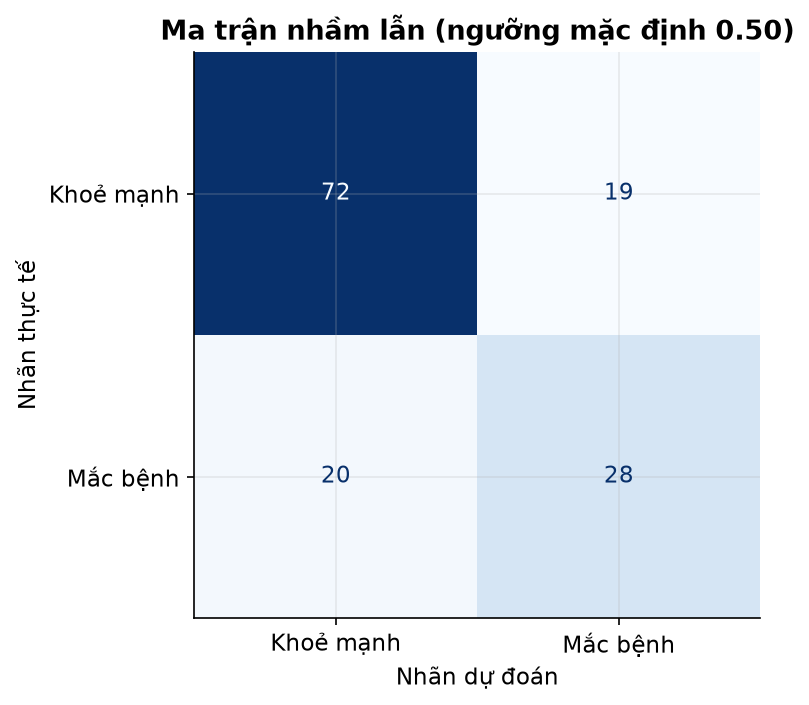
\includegraphics[width=\textwidth]{dia_confusion_default.png}
  \caption{Ngưỡng mặc định $\theta=0{,}50$}
  \label{fig:dia-cm-default}
\end{subfigure}
\hfill
\begin{subfigure}[b]{0.485\textwidth}
  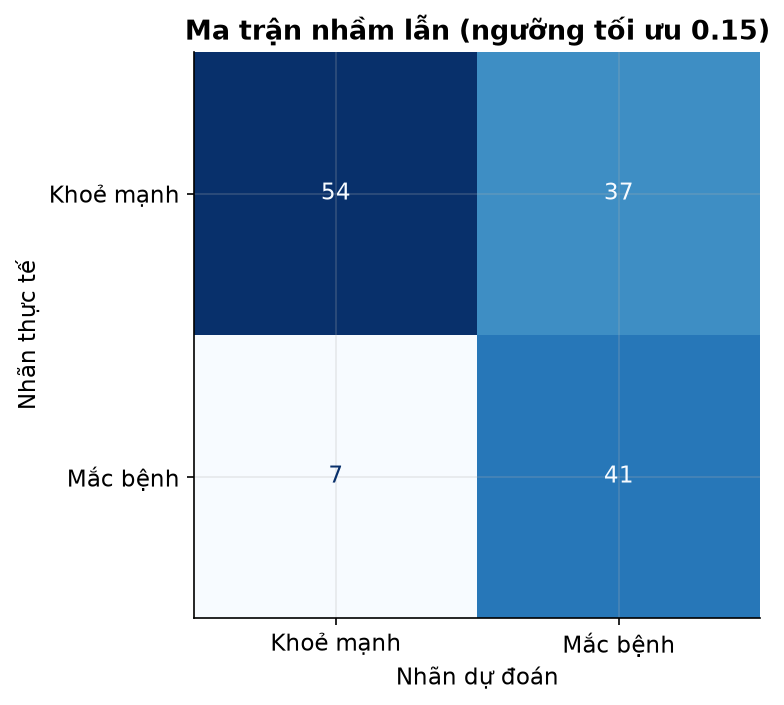
\includegraphics[width=\textwidth]{dia_confusion_tuned.png}
  \caption{Ngưỡng tối ưu $\theta=0{,}15$}
  \label{fig:dia-cm-tuned}
\end{subfigure}
\caption[Ma trận nhầm lẫn trước và sau khi hạ ngưỡng quyết định]%
{Ma trận nhầm lẫn của cùng một mô hình XGBoost, trước và sau khi hạ ngưỡng
quyết định}
\label{fig:dia-cm-pair}
\end{figure}

\nhanxet{Đọc thẳng từ Bảng~\ref{tab:threshold-dia}: hạ ngưỡng từ $0{,}50$ xuống
$0{,}15$ đưa số người bệnh bị bỏ sót từ \textbf{20 xuống 7} --- cứu được 13 ca
trên tổng số 48. Cái giá là số báo động nhầm tăng từ 19 lên 37, tức thêm 18
người khoẻ phải đi xét nghiệm lại.

Trong bài toán sàng lọc, đây là một đổi chác rõ ràng có lợi: một lần xét nghiệm
thừa tốn vài trăm nghìn đồng, còn một ca đái tháo đường bị bỏ sót có thể dẫn tới
biến chứng thận, mắt hoặc tim mạch sau nhiều năm. \textbf{Điểm quan trọng nhất:
mô hình không hề thay đổi} --- cùng bộ trọng số, cùng ROC-AUC $0{,}7905$. Thứ
thay đổi là chỗ ta cắt.}

\begin{phathien}{Hai bẫy phương pháp gặp phải trong chính thực nghiệm này}
\textbf{Bẫy 1 --- quét ngưỡng cần mô hình cho xác suất liên tục.} Bản chạy đầu
tiên thực hiện trên Decision Tree sâu 6 tầng. Bảy ngưỡng từ $0{,}50$ xuống
$0{,}20$ cho ra \emph{đúng một} kết quả giống hệt nhau. Nguyên nhân: cây nông
chỉ trả về vài giá trị xác suất rời rạc, nên phần lớn ngưỡng rơi vào cùng một
khoảng và không đổi được nhãn nào --- đúng hiện tượng đã thấy qua dạng gãy khúc
của đường ROC ở Hình~\ref{fig:dia-roc}. Chuyển sang XGBoost mới thấy được hiệu
ứng thật, với 12 mức kết quả khác nhau trên 13 ngưỡng.

\textbf{Bẫy 2 --- cực trị chạm biên dải khảo sát thì chưa phải cực trị.} Dải
quét ban đầu dừng ở $\theta=0{,}20$ và $F_1$ đạt đỉnh đúng tại đầu mút ấy. Chỉ
sau khi nới dải xuống $0{,}05$ mới xác nhận được đỉnh thật nằm ở $0{,}15$. Bẫy
này lặp lại lần thứ hai ở bài toán bất động sản với độ sâu rừng ngẫu nhiên ---
xem Mục~\ref{sec:tn2-hou}.
\end{phathien}

\section{Thực nghiệm 3 --- Ảnh hưởng của cách biểu diễn dữ liệu}
\label{sec:tn3-dia}

\textbf{Câu hỏi.} Giữ nguyên thuật toán, chỉ đổi cách biểu diễn --- kết quả thay
đổi bao nhiêu, và so với biên độ do đổi thuật toán thì thế nào?

\textbf{Thiết kế.} Bốn phương án biểu diễn, cùng chạy trên Logistic Regression,
cùng phép chia dữ liệu. Bốn phương án phản ánh đúng ba tầng chuyển hoá đã định
nghĩa ở Mục~\ref{sec:ba-tang-bieudien}.

\begin{table}[H]
\centering
\caption{Bốn phương án biểu diễn dữ liệu và kết quả trên Logistic Regression}
\label{tab:rep-dia}
\small
\begin{tabular}{@{}lrrrr@{}}
\toprule
\textbf{Phương án biểu diễn} & \textbf{Accuracy} & \textbf{Precision} & \textbf{Recall} & \textbf{$F_1$} \\
\midrule
Làm sạch, chưa chuẩn hoá                    & \textbf{0{,}8058} & 0{,}7561 & \textbf{0{,}6458} & \textbf{0{,}6966} \\
Thô --- giữ nguyên giá trị 0 phi lý         & 0{,}7986 & 0{,}7500 & 0{,}6250 & 0{,}6818 \\
Làm sạch $+$ chuẩn hoá                      & 0{,}7986 & 0{,}7500 & 0{,}6250 & 0{,}6818 \\
Làm sạch $+$ chuẩn hoá $+$ đặc trưng thiết kế & 0{,}7914 & 0{,}7436 & 0{,}6042 & 0{,}6667 \\
\bottomrule
\end{tabular}
\end{table}

\begin{figure}[H]
\centering
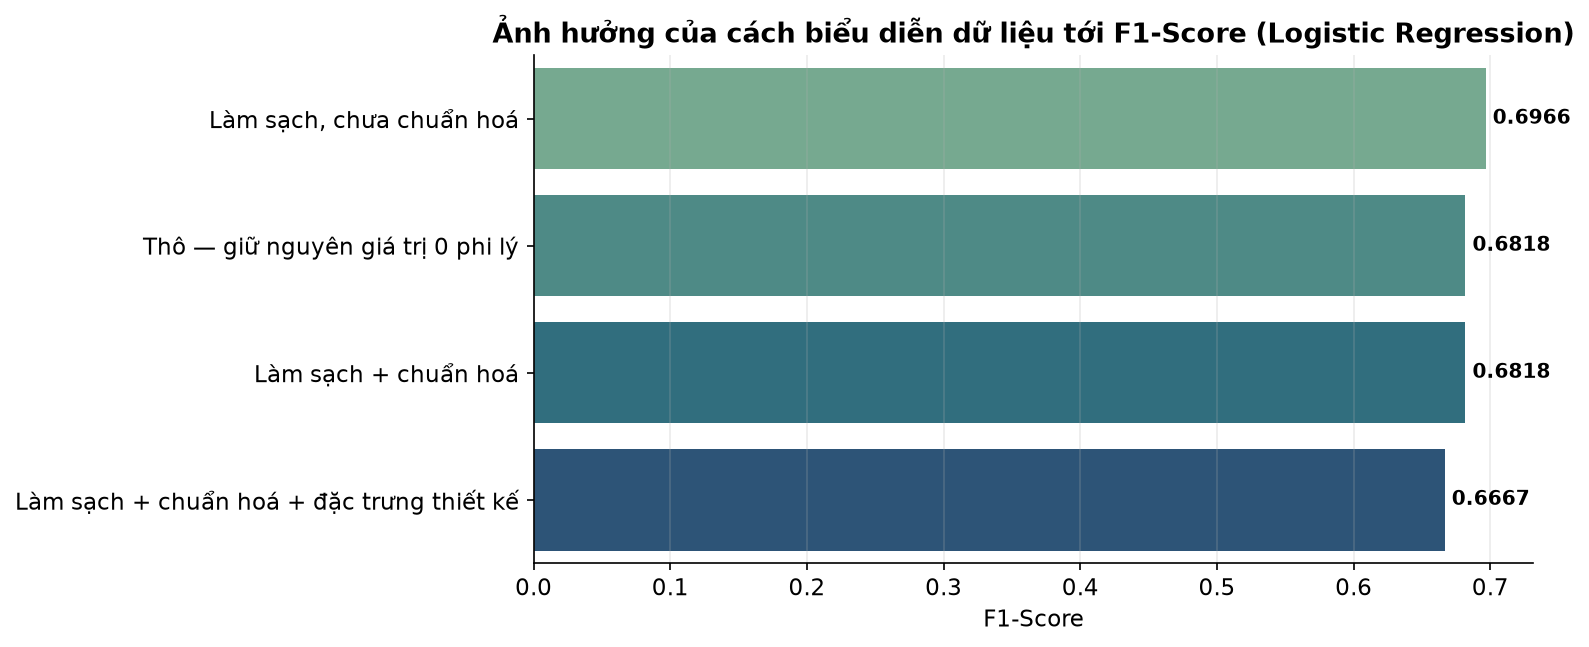
\includegraphics[width=\textwidth]{dia_representation.png}
\caption[Ảnh hưởng của cách biểu diễn dữ liệu tới $F_1$]%
{Ảnh hưởng của cách biểu diễn dữ liệu tới $F_1$ của Logistic Regression}
\label{fig:dia-representation}
\end{figure}

\bieudo{Biểu đồ cột ngang, sắp giảm dần theo $F_1$, giá trị ghi ở đầu mỗi cột.}

\phanphoi{Bốn cột gần bằng nhau. Khoảng cách giữa cột cao nhất và cột thấp nhất
nhỏ tới mức phải đọc con số mới thấy.}

\chitiet{$F_1$ trải từ $0{,}6667$ tới $0{,}6966$ --- biên độ $0{,}0300$. Hai
phương án giữa cho kết quả \emph{trùng khít nhau tới bốn chữ số thập phân}
($0{,}6818$), tức việc chuẩn hoá không đổi được một ca nào.}

\begin{phathien}{Kết quả đi ngược giả thuyết ban đầu --- và đây là phát hiện chính}
\label{sec:dactrung-tot}
Giả thuyết trước khi chạy là biểu diễn tốt hơn sẽ cho kết quả tốt hơn, với
phương án đầy đủ nhất đứng đầu. Kết quả \textbf{ngược lại}: phương án đầy đủ
nhất --- có cả chuẩn hoá lẫn bốn đặc trưng thiết kế --- xếp \textbf{cuối cùng}.

Ba lời giải thích, mỗi lời giải thích kiểm chứng được:

\begin{enumerate}
  \item \textbf{Chuẩn hoá không giúp gì cho Logistic Regression ở đây.} Hai
        phương án ``có'' và ``không có'' chuẩn hoá cho kết quả trùng khít. Điều
        này đúng lý thuyết: hồi quy logistic không dựa trên khoảng cách, phép
        chuẩn hoá tuyến tính chỉ đổi thang trọng số chứ không đổi ranh giới
        quyết định. Nó \emph{bắt buộc} với K-Nearest Neighbors, nhưng vô hại và
        vô ích với mô hình này.
  \item \textbf{Đặc trưng thiết kế \emph{làm hại} Logistic Regression.} $F_1$
        giảm từ $0{,}6818$ xuống $0{,}6667$. Nguyên nhân là đa cộng tuyến dưới
        phạt $L_2$: \texttt{Glucose\_BMI\_Risk} tương quan $0{,}82$ với
        \texttt{Glucose} và $0{,}73$ với \texttt{BMI}
        (Hình~\ref{fig:dia-corr}), nên số hạng
        $\lambda\lVert\bm\theta\rVert_2^2$ ở~\eqref{eq:regularized} phân tán
        trọng số ra ba cột gần trùng nhau thay vì dồn vào một cột.
  \item \textbf{Toàn bộ biên độ nằm trong nhiễu lấy mẫu.} $0{,}0300$ $F_1$ trên
        139 ca kiểm tra tương ứng chênh lệch chỉ \textbf{1--9 ca} giữa các
        phương án. Không phương án nào tách khỏi phần còn lại một cách có ý
        nghĩa thống kê.
\end{enumerate}

\textbf{Hệ quả khái quát:} ``đặc trưng tốt'' không phải thuộc tính của riêng đặc
trưng, mà là thuộc tính của \emph{cặp đặc trưng -- thuật toán}. Chính
\texttt{Glucose\_BMI\_Risk} vừa là đặc trưng tương quan mạnh nhất với nhãn
($0{,}5199$) vừa là đặc trưng quan trọng nhất của XGBoost ($0{,}1874$, xem
Hình~\ref{fig:dia-importance}) --- nhưng lại làm Logistic Regression kém đi.
\end{phathien}

\subsection{So sánh biên độ: biểu diễn hay thuật toán?}

\begin{table}[H]
\centering
\caption{Biên độ do đổi biểu diễn so với biên độ do đổi thuật toán, bài toán tiểu đường}
\label{tab:biendo-dia}
\small
\begin{tabular}{@{}lrl@{}}
\toprule
\textbf{Nguồn biến thiên} & \textbf{Biên độ $F_1$} & \textbf{Ghi chú} \\
\midrule
Đổi cách biểu diễn (4 phương án) & 0{,}0300 & $0{,}6667 \to 0{,}6966$ \\
Đổi thuật toán (5 mô hình)       & \textbf{0{,}1809} & $0{,}5000 \to 0{,}6809$ \\
\midrule
\textbf{Tỷ số} & \multicolumn{2}{l}{\textbf{Thuật toán chi phối, gấp 6 lần}} \\
\bottomrule
\end{tabular}
\end{table}

Kết luận này sẽ được đối chiếu với kết quả \emph{trái ngược} ở bài toán bất động
sản tại Mục~\ref{sec:phanchieu}.

\section{Thực nghiệm 4 --- Kiểm chuẩn ngoài phân phối}
\label{sec:tn4-dia}

\textbf{Câu hỏi.} Điểm số trên tập kiểm tra có lạc quan quá không?

\begin{figure}[H]
\centering
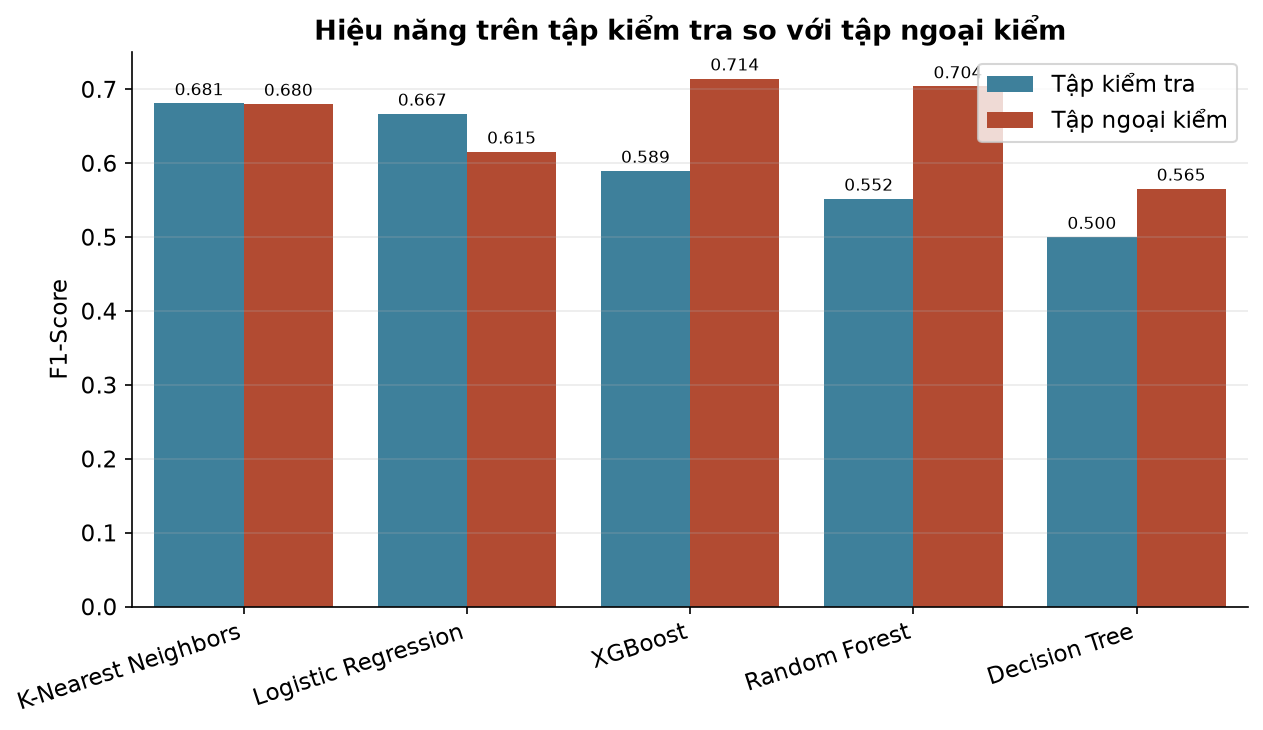
\includegraphics[width=0.92\textwidth]{dia_ood_comparison.png}
\caption[So sánh $F_1$ giữa tập kiểm tra và tập ngoại kiểm]%
{So sánh $F_1$ của năm mô hình giữa tập kiểm tra và tập ngoại kiểm}
\label{fig:dia-ood}
\end{figure}

\begin{table}[H]
\centering
\caption{Kết quả trên tập ngoại kiểm (77 ca chưa từng dùng trong phát triển)}
\label{tab:ood-dia}
\small
\begin{tabular}{@{}lrrrrr@{}}
\toprule
\textbf{Mô hình} & \textbf{Accuracy} & \textbf{Precision} & \textbf{Recall} & \textbf{$F_1$} & \textbf{ROC-AUC} \\
\midrule
XGBoost             & \textbf{0{,}7922} & 0{,}6897 & \textbf{0{,}7407} & \textbf{0{,}7143} & 0{,}8800 \\
Random Forest       & \textbf{0{,}7922} & 0{,}7037 & 0{,}7037 & 0{,}7037 & \textbf{0{,}8904} \\
K-Nearest Neighbors & \textbf{0{,}7922} & \textbf{0{,}7391} & 0{,}6296 & 0{,}6800 & \textbf{0{,}8904} \\
Logistic Regression & 0{,}7403 & 0{,}6400 & 0{,}5926 & 0{,}6154 & 0{,}8511 \\
Decision Tree       & 0{,}7403 & 0{,}6842 & 0{,}4815 & 0{,}5652 & 0{,}7774 \\
\bottomrule
\end{tabular}
\end{table}

\nhanxet{Kết quả trên tập ngoại kiểm \textbf{cao hơn} tập kiểm tra ở hầu hết mô
hình --- XGBoost tăng $F_1$ từ $0{,}5895$ lên $0{,}7143$. Đây không phải bằng
chứng mô hình tổng quát hoá xuất sắc; nó chủ yếu là dao động lấy mẫu trên một
tập chỉ 77 ca. Điều đáng tin hơn là \emph{thứ hạng đảo lộn}: XGBoost từ hạng ba
lên hạng nhất, Logistic Regression từ hạng hai xuống hạng tư.

Hệ quả phương pháp: chênh lệch $F_1$ dưới khoảng $0{,}05$ giữa hai mô hình trên
tập cỡ này \textbf{không đủ để kết luận mô hình nào tốt hơn}. Đây cũng là lý do
Mục~\ref{sec:tn3-dia} không tuyên bố phương án biểu diễn nào thắng.}

\section{Mức độ quan trọng của đặc trưng}
\label{sec:importance-dia}

\begin{figure}[H]
\centering
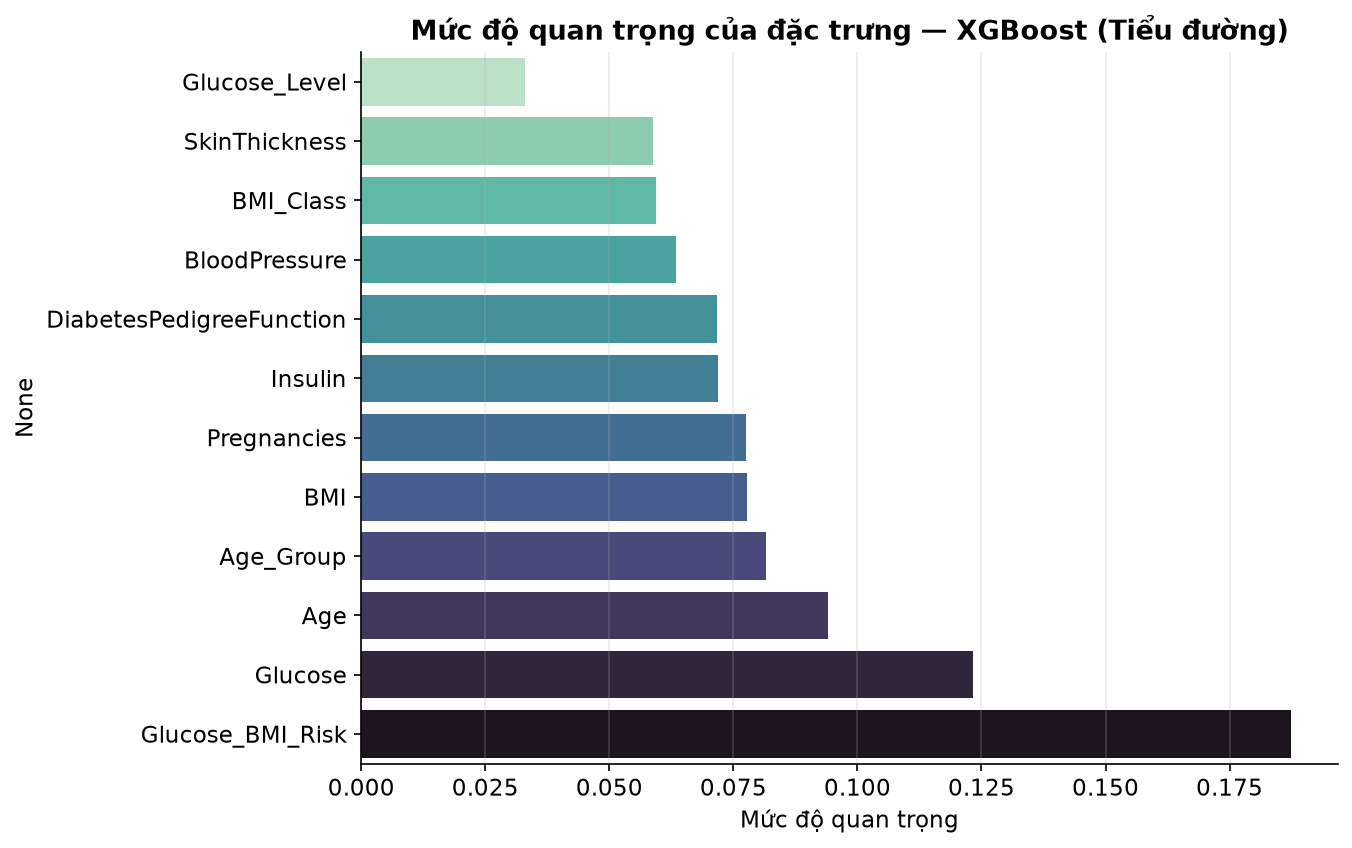
\includegraphics[width=0.88\textwidth]{dia_feature_importance.png}
\caption[Mức độ quan trọng của đặc trưng theo XGBoost]%
{Mức độ quan trọng của đặc trưng theo mô hình XGBoost}
\label{fig:dia-importance}
\end{figure}

\bieudo{Biểu đồ cột ngang, sắp tăng dần từ trên xuống. Độ quan trọng đo bằng
mức giảm độ vẩn tích luỹ mà mỗi đặc trưng mang lại qua toàn bộ cây.}

\phanphoi{Phân bố khá đều, không có đặc trưng nào áp đảo. Hai cột đầu tách khỏi
phần còn lại, chín cột sau tạo thành một dải liên tục.}

\chitiet{\texttt{Glucose\_BMI\_Risk} dẫn đầu với $0{,}1874$, kế đến
\texttt{Glucose} gốc $0{,}1233$. Nhóm giữa gồm \texttt{Age} $0{,}0940$,
\texttt{Age\_Group} $0{,}0815$, \texttt{BMI} $0{,}0778$ và \texttt{Pregnancies}
$0{,}0776$. Cuối bảng là \texttt{Glucose\_Level} với $0{,}0330$.}

\nhanxet{Ba quan sát.

\textbf{(1) Đặc trưng thiết kế đứng đầu} --- bằng chứng thứ hai (sau
Bảng~\ref{tab:corr-dia}) rằng tri thức y học đưa vào đúng chỗ có giá trị đo
được, ít nhất là với mô hình cây.

\textbf{(2) Rời rạc hoá làm mất thông tin với mô hình cây.}
\texttt{Glucose\_Level} xếp cuối trong khi \texttt{Glucose} gốc xếp thứ hai.
Điều này hợp lý: cây quyết định \emph{tự} tìm ngưỡng chia tối ưu trên biến liên
tục, nên việc rời rạc hoá thủ công thành ba mức chỉ giới hạn không gian tìm kiếm
của nó. Rời rạc hoá có ích cho mô hình tuyến tính, không có ích cho cây.

\textbf{(3) Không có đặc trưng nào vượt $0{,}19$} --- tín hiệu phân tán mỏng
trên nhiều biến. Điều này giải thích vì sao trần hiệu năng trên tập Pima nằm ở
mức $0{,}77$--$0{,}79$ Accuracy trong toàn bộ tài liệu công bố, và vì sao mọi
kết quả vượt xa mốc ấy đều đáng nghi (xem lại khung ở Mục~\ref{sec:roro}).}

\section{Tích hợp Đồ thị Tri thức Y sinh}
\label{sec:kg-dia}

\subsection{Từ xác suất tới tầng nguy cơ}

Ngưỡng phân tầng lấy trực tiếp từ Thực nghiệm~2, không phải chọn tuỳ ý:

\begin{table}[H]
\centering
\caption{Ba tầng nguy cơ lâm sàng và ánh xạ sang mã bệnh quốc tế}
\label{tab:tang-dia}
\small
\begin{tabularx}{\textwidth}{@{}L{3.6cm}L{1.7cm}L{1.7cm}X@{}}
\toprule
\textbf{Tầng nguy cơ} & \textbf{Ngưỡng $\hat p$} & \textbf{ICD-10} & \textbf{Tên mã bệnh} \\
\midrule
Nhóm Nguy cơ Cao        & $\ge 0{,}25$ & E11   & Đái tháo đường Type 2 \\
Nhóm Tiền Đái tháo đường & $\ge 0{,}15$ & R73.0 & Tăng glucose máu bất thường \\
Nhóm Khoẻ mạnh          & $\ge 0{,}00$ & Z13.1 & Khám sàng lọc đái tháo đường \\
\bottomrule
\end{tabularx}
\end{table}

\subsection{Đồ thị của một ca cụ thể}

\begin{figure}[H]
\centering
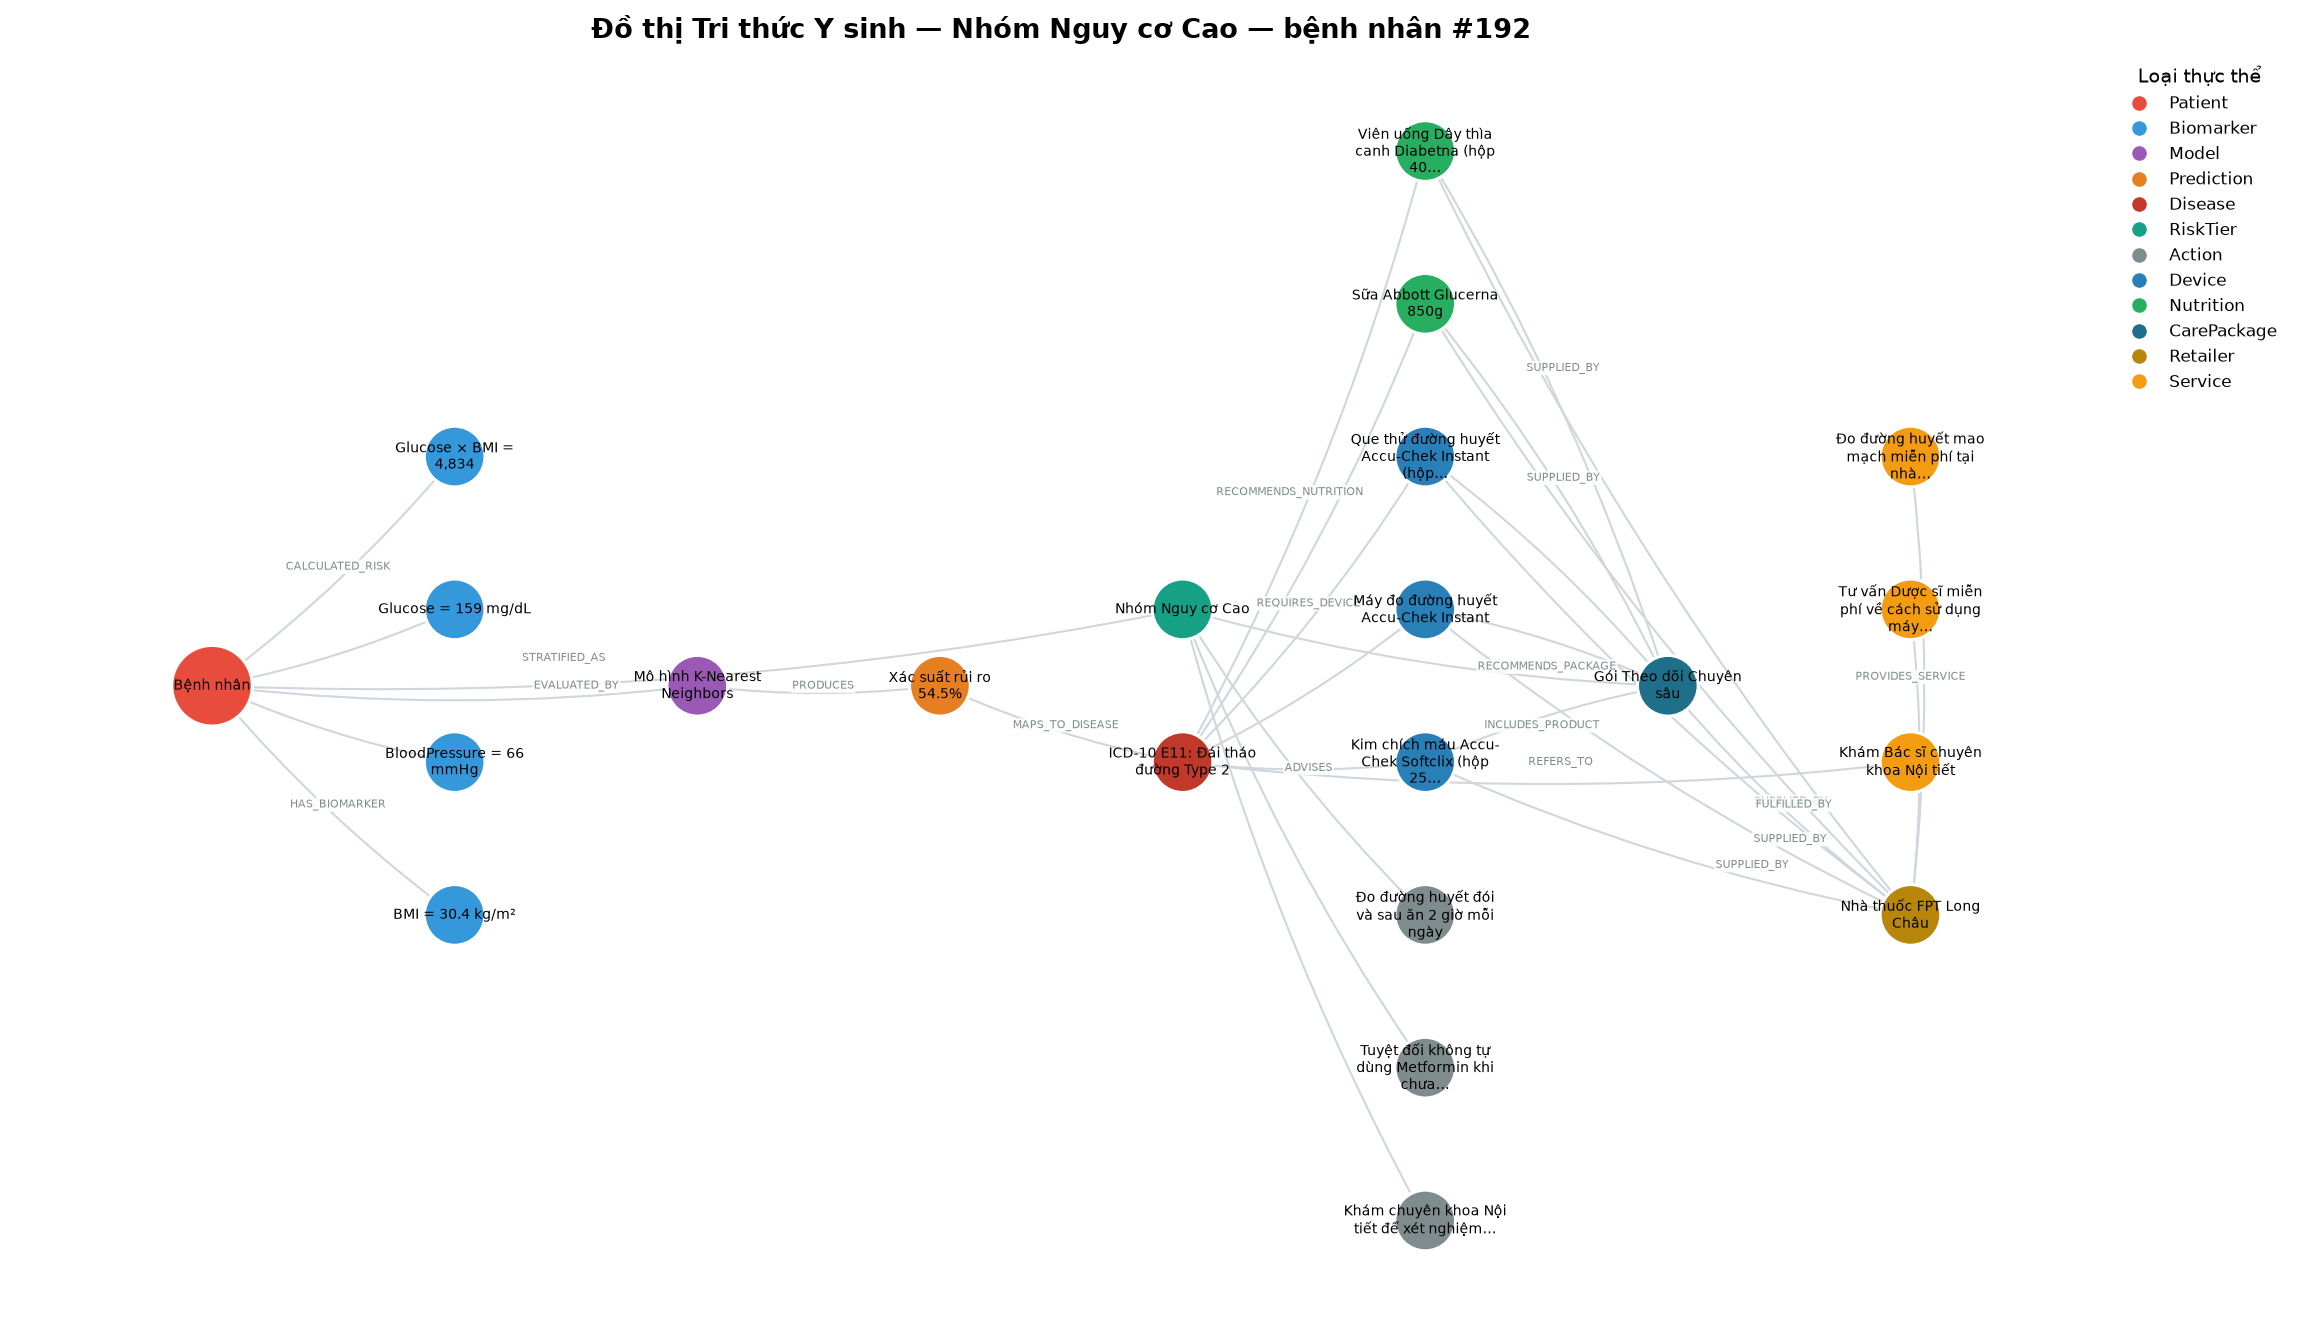
\includegraphics[width=\textwidth]{kg_medical.png}
\caption[Đồ thị Tri thức Y sinh của bệnh nhân \#192]%
{Đồ thị Tri thức Y sinh của bệnh nhân \#192 --- Nhóm Nguy cơ Cao, 22 thực thể
và 31 cạnh}
\label{fig:kg-medical}
\end{figure}

\bieudo{Đồ thị có hướng vẽ theo bố cục phân tầng (layered graph layout). Màu nút
mã hoá loại thực thể theo chú giải bên phải, nhãn trên cạnh là tên quan hệ.}

\phanphoi{Cấu trúc hình quạt mở dần từ trái sang phải: một nút gốc duy nhất
(Bệnh nhân) phân nhánh qua các tầng suy luận rồi mở rộng ra tầng hàng hoá và
dịch vụ.}

\chitiet{Tầng 1 bên trái gồm bốn chỉ số sinh học cùng đặc trưng tương tác
$\text{Glucose}\times\text{BMI}=4.834$. Tầng 2 ở giữa là chuỗi Mô hình
K-Nearest Neighbors $\to$ Xác suất $54{,}5\%$ $\to$ ICD-10 E11 $\to$ Nhóm Nguy
cơ Cao. Tầng 3 toả ra ba nhóm: hai thiết bị, ba mặt hàng dinh dưỡng, ba hướng
dẫn lâm sàng. Tầng 4 gom lại thành một nút Gói Theo dõi Chuyên sâu. Tầng 5 bên
phải hội tụ về nút Nhà thuốc FPT Long Châu cùng hai dịch vụ tại quầy và một
đường chuyển tuyến chuyên khoa.}

\subsection{Chuỗi suy luận đầy đủ}

\begin{table}[H]
\centering
\caption{Chuỗi bộ ba tri thức của bệnh nhân \#192, từ số đo tới nơi mua hàng}
\label{tab:triplet-dia}
\scriptsize
\begin{tabularx}{\textwidth}{@{}L{4.1cm}L{3.5cm}X@{}}
\toprule
\textbf{Chủ thể} & \textbf{Quan hệ} & \textbf{Đối tượng} \\
\midrule
Bệnh nhân & \texttt{HAS\_BIOMARKER} & Glucose $=159$ mg/dL \\
Bệnh nhân & \texttt{HAS\_BIOMARKER} & BMI $=30{,}4$ kg/m$^2$ \\
Bệnh nhân & \texttt{CALCULATED\_RISK} & Glucose $\times$ BMI $=4.834$ \\
Bệnh nhân & \texttt{EVALUATED\_BY} & Mô hình K-Nearest Neighbors \\
Mô hình K-Nearest Neighbors & \texttt{PRODUCES} & Xác suất rủi ro $54{,}5\%$ \\
Xác suất rủi ro $54{,}5\%$ & \texttt{MAPS\_TO\_DISEASE} & ICD-10 E11 \\
Bệnh nhân & \texttt{STRATIFIED\_AS} & Nhóm Nguy cơ Cao \\
ICD-10 E11 & \texttt{REQUIRES\_DEVICE} & Máy đo đường huyết Accu-Chek Instant \\
ICD-10 E11 & \texttt{RECOMMENDS\_NUTRITION} & Sữa Abbott Glucerna 850g \\
Nhóm Nguy cơ Cao & \texttt{ADVISES} & Khám chuyên khoa Nội tiết \\
Nhóm Nguy cơ Cao & \texttt{RECOMMENDS\_PACKAGE} & \textbf{Gói Theo dõi Chuyên sâu} \\
Gói Theo dõi Chuyên sâu & \texttt{INCLUDES\_PRODUCT} & (5 mặt hàng) \\
Gói Theo dõi Chuyên sâu & \texttt{FULFILLED\_BY} & \textbf{Nhà thuốc FPT Long Châu} \\
Nhà thuốc FPT Long Châu & \texttt{PROVIDES\_SERVICE} & Đo đường huyết miễn phí tại quầy \\
ICD-10 E11 & \texttt{REFERS\_TO} & Khám Bác sĩ chuyên khoa Nội tiết \\
\bottomrule
\end{tabularx}
\end{table}

\subsection{Gói chăm sóc sức khoẻ và giải pháp dược phẩm}
\label{sec:goi-cham-soc}

Đây là điểm mà hệ thống trả lời được câu hỏi cuối cùng của người dùng:
\emph{vậy tôi phải mua gì, và hết bao nhiêu tiền}.

\begin{table}[H]
\centering
\caption{Gói Theo dõi Chuyên sâu --- danh mục mặt hàng cho Nhóm Nguy cơ Cao}
\label{tab:goi-cao}
\scriptsize
\begin{tabularx}{\textwidth}{@{}L{1.9cm}XL{2.6cm}L{1.35cm}@{}}
\toprule
\textbf{Mã SKU} & \textbf{Mặt hàng} & \textbf{Khoảng giá} & \textbf{Định kỳ} \\
\midrule
LC-DEV-001 & Máy đo đường huyết Accu-Chek Instant        & 790.000 -- 1.090.000 đ & Không \\
LC-DEV-002 & Que thử đường huyết Accu-Chek (hộp 50 que)  & 300.000 -- 420.000 đ   & Có \\
LC-DEV-003 & Kim chích máu Accu-Chek Softclix (hộp 25)   & 90.000 -- 150.000 đ    & Có \\
LC-NUT-001 & Sữa Abbott Glucerna 850g                    & 690.000 -- 890.000 đ   & Có \\
LC-NUT-003 & Viên uống Dây thìa canh Diabetna (hộp 40)   & 120.000 -- 195.000 đ   & Có \\
\midrule
\multicolumn{2}{@{}l}{\textbf{Chi phí ban đầu}}          & \textbf{1.990.000 -- 2.745.000 đ} & \\
\multicolumn{2}{@{}l}{\textbf{Duy trì hằng tháng}}       & \textbf{1.200.000 -- 1.655.000 đ} & \\
\multicolumn{2}{@{}l}{\textbf{Tổng 12 tháng đầu}}        & \textbf{15.190.000 -- 20.950.000 đ} & \\
\bottomrule
\end{tabularx}
\end{table}

\begin{table}[H]
\centering
\caption{Ba gói chăm sóc theo tầng nguy cơ}
\label{tab:ba-goi}
\small
\begin{tabularx}{\textwidth}{@{}L{3.9cm}rL{2.8cm}X@{}}
\toprule
\textbf{Gói} & \textbf{Số mặt hàng} & \textbf{Chi phí ban đầu} & \textbf{Tần suất theo dõi} \\
\midrule
Theo dõi Chuyên sâu       & 5 & 1{,}99 -- 2{,}75 tr.đ & Đo đường huyết đói và sau ăn 2 giờ, mỗi ngày \\
Dự phòng Tiền Đái tháo đường & 4 & 1{,}43 -- 2{,}08 tr.đ & Kiểm tra lại đường huyết sau 3 tháng \\
Duy trì Sức khoẻ          & 1 & 0{,}15 -- 0{,}32 tr.đ & Khám sức khoẻ định kỳ hằng năm \\
\bottomrule
\end{tabularx}
\end{table}

\nhanxet{Chi phí ban đầu và chi phí duy trì được tách riêng có chủ đích. Gói
Theo dõi Chuyên sâu có máy đo là khoản mua một lần trị giá tới $1{,}09$ triệu
đồng; gộp chung hai con số sẽ khiến gói trông đắt gấp rưỡi thực tế của tháng thứ
hai trở đi. Đây là loại minh bạch mà một bảng khuyến nghị chỉ liệt kê tên hàng
không thể cung cấp.

Về nguồn số liệu, xin nhắc lại ranh giới đã nêu ở Mục~\ref{sec:ranh-gioi-so-lieu}:
tên mặt hàng là tên thật, giá là khoảng tham khảo chốt ngày 26/08/2026, và mỗi
mặt hàng mang một đường dẫn tra cứu giá hiện hành. Thuốc kê đơn --- Metformin và
nhóm hạ đường huyết khác --- \textbf{không} nằm trong danh mục này; đồ thị chỉ
ghi lời khuyến cáo ``tuyệt đối không tự dùng khi chưa có chỉ định bác sĩ''.}

\section{Ứng dụng web}
\label{sec:app-dia}

\begin{figure}[H]
\centering
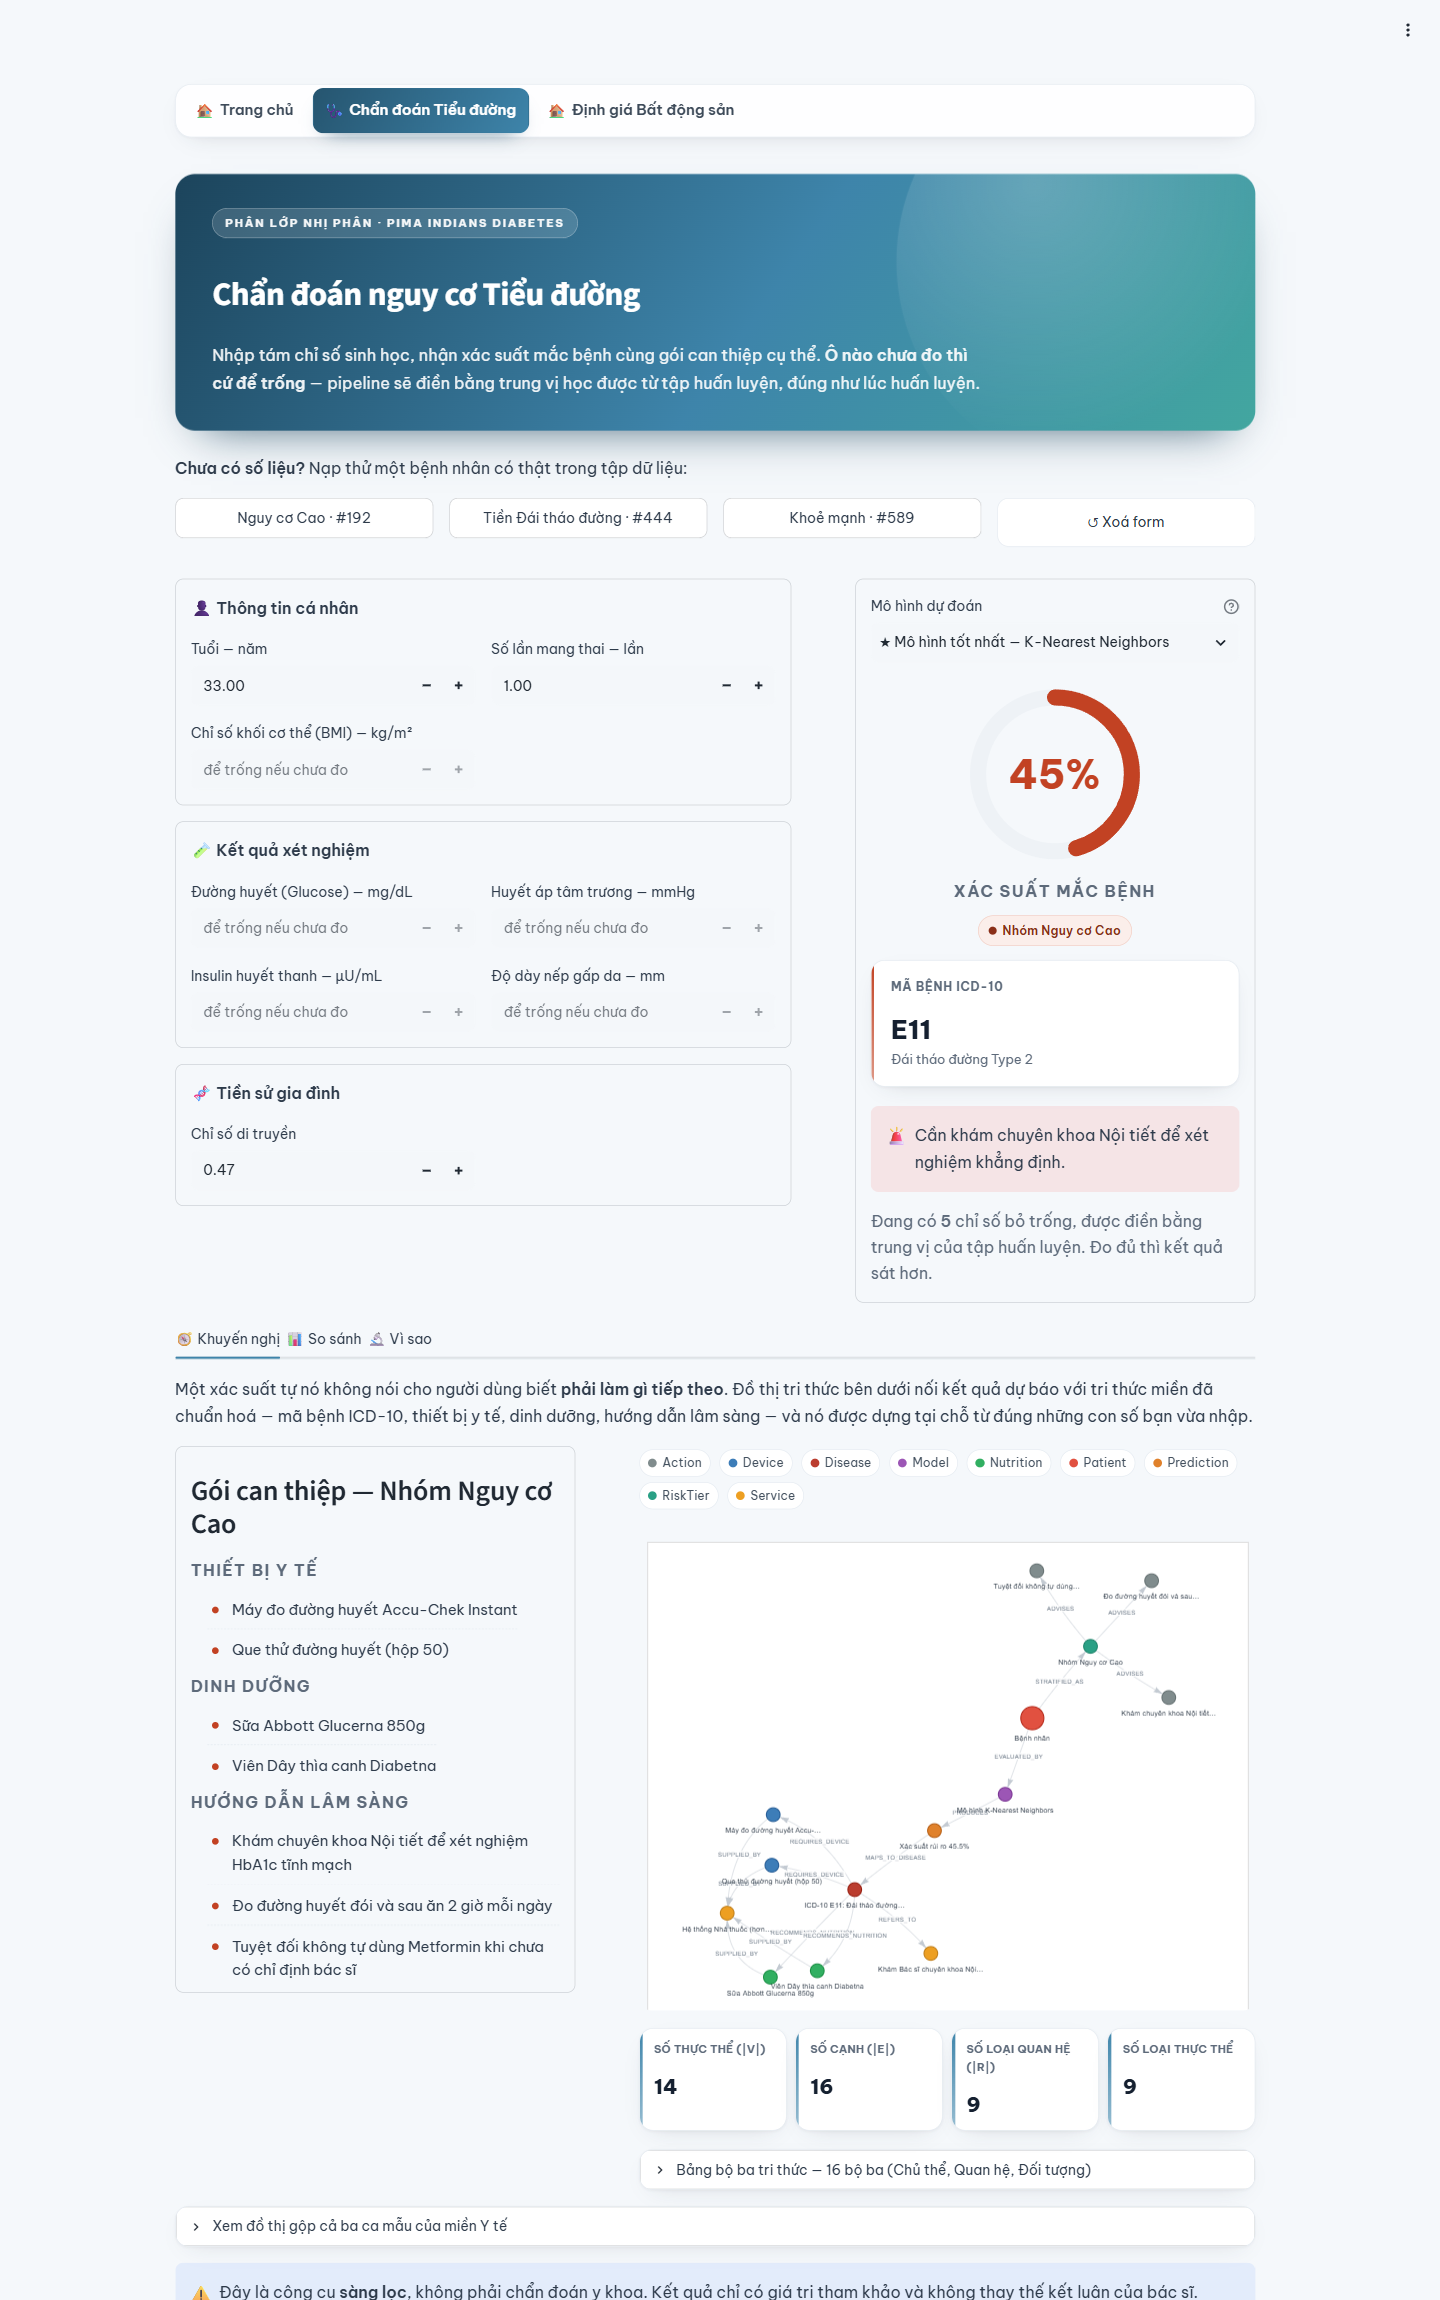
\includegraphics[width=0.86\textwidth]{app-desktop-2-chan-doan.png}
\caption[Giao diện trang Chẩn đoán Tiểu đường trên máy tính]%
{Giao diện trang Chẩn đoán Tiểu đường trên máy tính --- biểu mẫu nhập liệu, kết
quả dự báo và đồ thị tri thức dựng tại chỗ}
\label{fig:app-dia-desktop}
\end{figure}

\bieudo{Ảnh chụp màn hình bản đã triển khai công khai, khổ máy tính $1440$ px.}

\chitiet{Bố cục hai cột. Cột trái là biểu mẫu chia ba khối --- thông tin cá
nhân, kết quả xét nghiệm, tiền sử gia đình --- với ô để trống được xử lý như dữ
liệu khuyết chứ không phải giá trị $0$. Cột phải hiển thị vòng tròn xác suất,
nhãn tầng nguy cơ, mã ICD-10 và cảnh báo chuyển tuyến. Phía dưới là bốn tab:
Khuyến nghị, Gói chăm sóc, So sánh, Vì sao.}

\nhanxet{Ứng dụng nạp lại đúng các tệp \texttt{models/*.joblib} do
\texttt{run\_pipeline.py} sinh ra, nên biểu diễn lúc dự đoán trùng khít biểu
diễn lúc huấn luyện --- toàn bộ bước điền khuyết, thiết kế đặc trưng và chuẩn
hoá đều nằm bên trong \texttt{Pipeline} được lưu.

Chi tiết đáng chú ý về mặt thiết kế: khi người dùng để trống một ô, ứng dụng
hiển thị dòng cảnh báo cho biết có bao nhiêu chỉ số đang được điền bằng trung vị
của tập huấn luyện. Điều này giữ cho người dùng biết mức độ tin cậy của con số
họ vừa nhận --- một dự báo dựa trên 8 chỉ số đo đủ khác hẳn một dự báo mà 5
trong 8 chỉ số là giá trị điền.}

\begin{figure}[H]
\centering
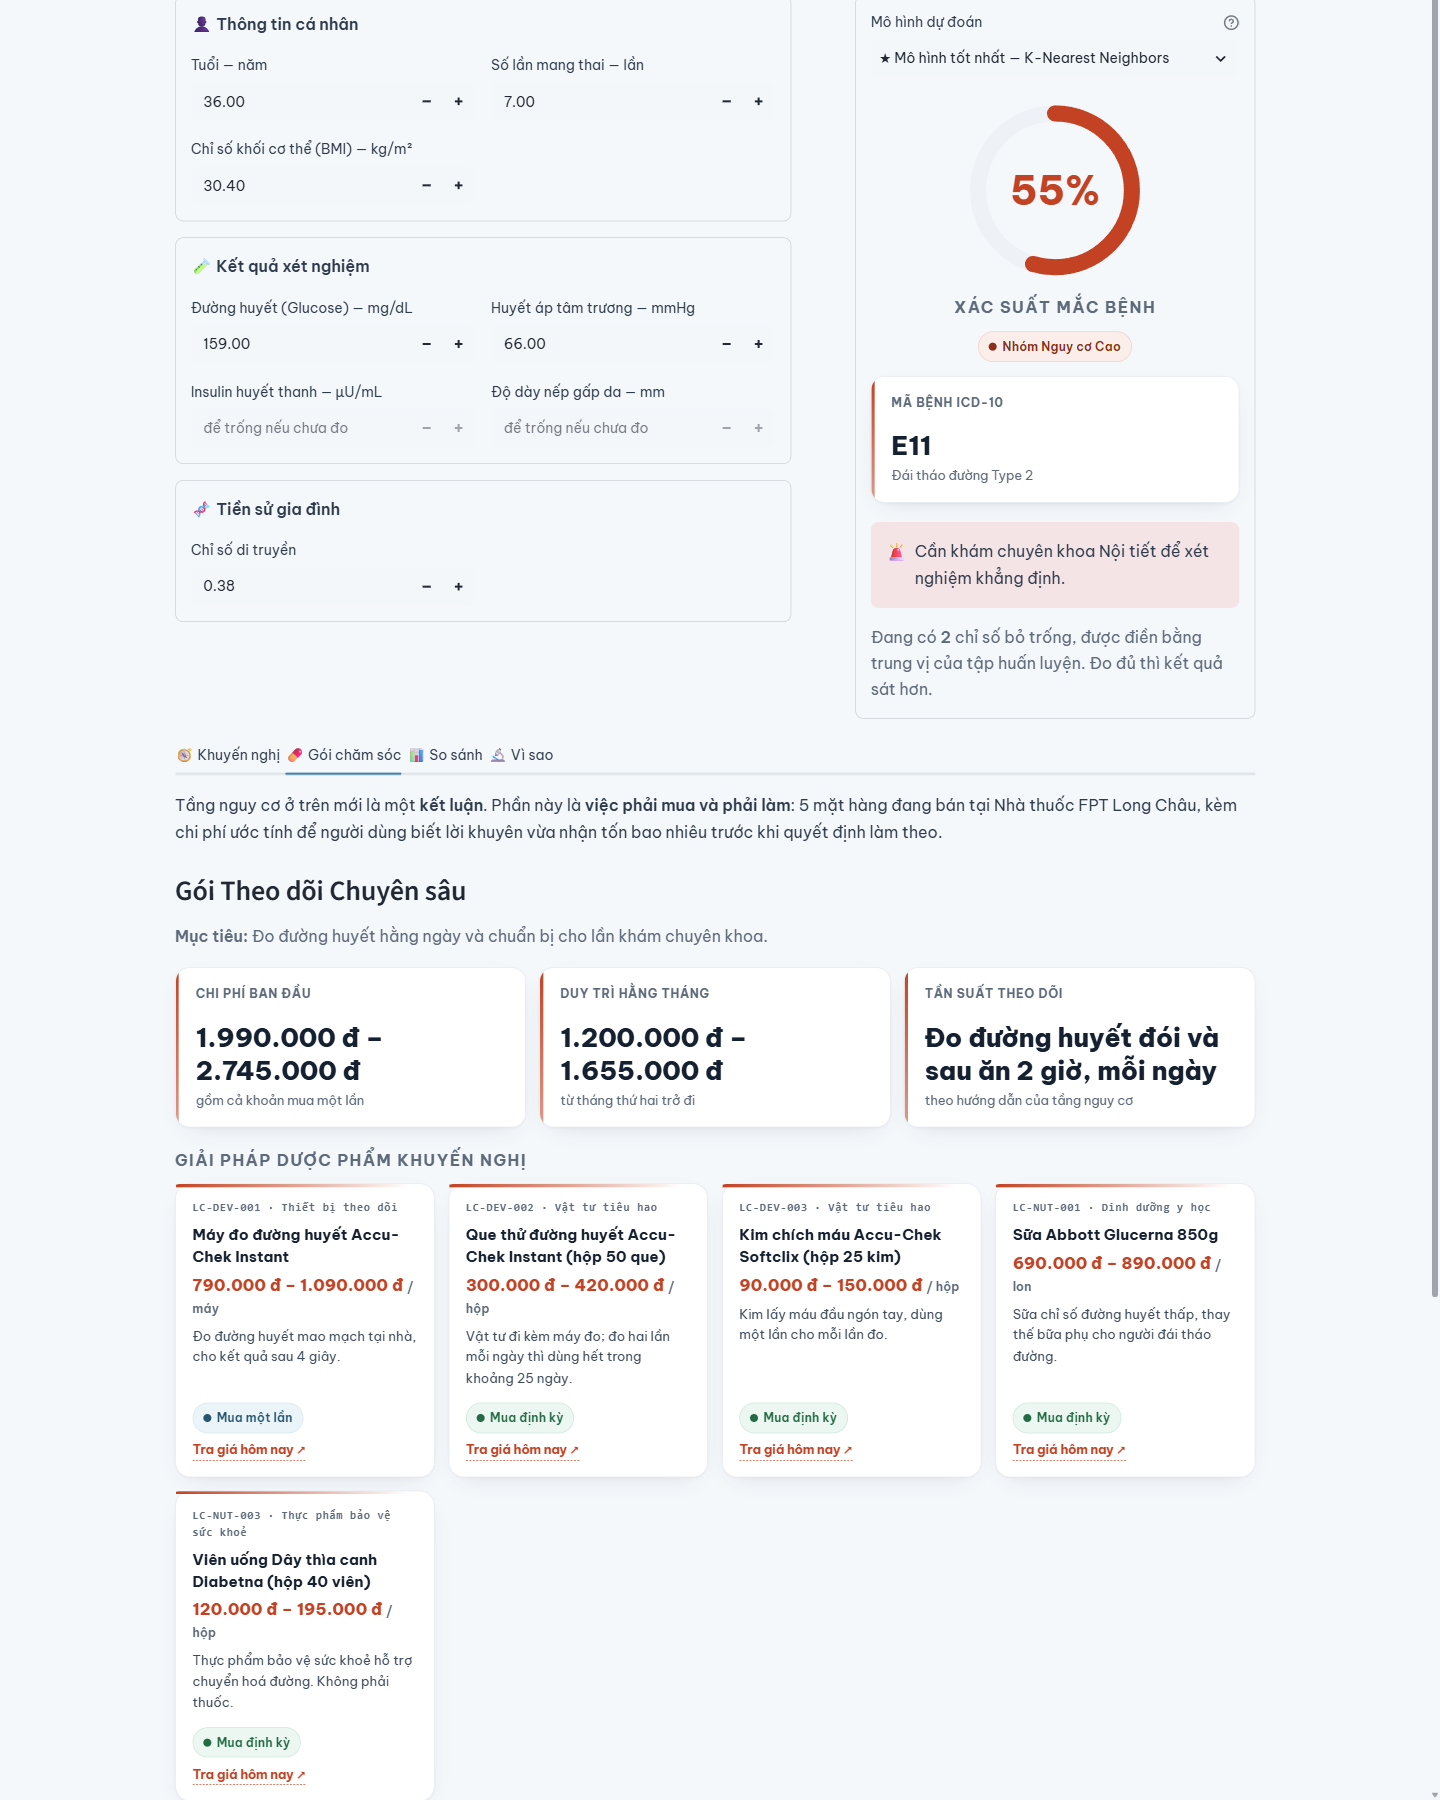
\includegraphics[width=0.86\textwidth]{app-desktop-4-goi-cham-soc.png}
\caption[Tab Gói chăm sóc --- giải pháp dược phẩm khuyến nghị]%
{Tab \emph{Gói chăm sóc} --- năm mặt hàng của Gói Theo dõi Chuyên sâu, mỗi thẻ
mang mã SKU, khoảng giá và đường dẫn tra giá hiện hành}
\label{fig:app-dia-goi}
\end{figure}

\bieudo{Ảnh chụp màn hình tab thứ hai của trang Chẩn đoán.}

\chitiet{Phần trên là biểu mẫu đã nạp sẵn hồ sơ bệnh nhân \#192 --- Glucose
$159$ mg/dL, BMI $30{,}4$ --- cùng kết quả $55\%$ và mã ICD-10 E11. Trong tab,
ba thẻ số cho chi phí ban đầu $1{,}99$--$2{,}75$ triệu đồng, chi phí duy trì
$1{,}20$--$1{,}66$ triệu đồng mỗi tháng, và tần suất theo dõi. Bên dưới là lưới
năm thẻ mặt hàng, mỗi thẻ ghi mã SKU, nhóm hàng, khoảng giá theo đơn vị bán,
công dụng, nhãn ``mua một lần'' hoặc ``mua định kỳ'', và một liên kết tra giá.
Cuộn tiếp xuống dưới khung hình còn có bảng tóm tắt nhà thuốc --- với con số chi
phí 12 tháng đầu $15{,}19$--$20{,}95$ triệu đồng --- và khung cảnh báo nguồn giá.}

\nhanxet{Khung cảnh báo ở cuối tab là phần không được lược bỏ: nó nêu rõ ngày
chốt giá, nói rằng đây là gợi ý mua sắm chứ \textbf{không phải đơn thuốc}, và
nhắc rằng thuốc kê đơn không nằm trong danh mục. Một giao diện bán hàng bỏ dòng
này đi sẽ biến một công cụ sàng lọc thành một quảng cáo dược phẩm.}

\begin{figure}[H]
\centering
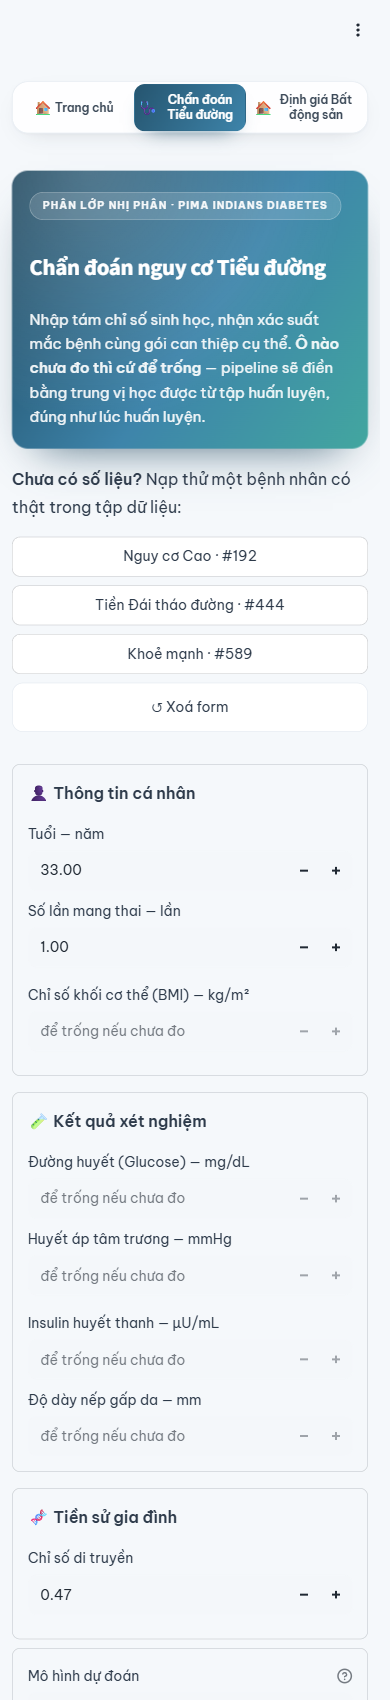
\includegraphics[width=0.34\textwidth]{app-mobile-2-chan-doan.png}
\caption[Giao diện trang Chẩn đoán trên điện thoại]%
{Giao diện trang Chẩn đoán trên điện thoại, khổ $390$ px --- biểu mẫu xếp dọc,
thanh điều hướng tự xuống dòng}
\label{fig:app-dia-mobile}
\end{figure}

% =====================================================================
%  Chương 3 — Hệ thống Định giá Bất động sản Việt Nam
% =====================================================================
\chapter{Hệ thống Định giá Bất động sản Việt Nam}
\label{ch:batdongsan}

\section{Phát biểu bài toán}
\label{sec:phatbieu-hou}

\subsection{Hiện tượng thực tế và người dùng}

Thị trường nhà đất Việt Nam thiếu một mức giá tham chiếu công khai. Người mua
dựa vào giá rao của người bán, người bán dựa vào giá rao của hàng xóm, và cả hai
bên đều không có cách kiểm chứng độc lập. Hệ quả là khoảng chênh lệch thương
lượng rất rộng, và bên nào ít thông tin hơn thì chịu thiệt.

Một hệ thống định giá tự động không thay thế được thẩm định giá chính thức ---
việc ấy đòi hỏi khảo sát hiện trạng --- nhưng nó cung cấp được \textbf{mốc tham
chiếu độc lập} dựng từ 30.229 giao dịch thật, cùng với điều mà một con số giá
đơn lẻ không nói được: vay được bao nhiêu, trả góp thế nào, và quanh đó có gì.

\subsection{Phát biểu hình thức}

Cho một hồ sơ bất động sản $\mathbf{x}$ gồm thuộc tính vật lý, vị trí hành chính
và tình trạng pháp lý, hãy học hàm

\begin{equation}
f_{\bm\theta}:\ \mathcal{X}\longrightarrow\mathbb{R}_{+},
\qquad
\hat y = f_{\bm\theta}(\mathbf{x}) \approx \texttt{Price}\ \text{(tỷ VNĐ)},
\label{eq:baitoan-hou}
\end{equation}

\noindent sao cho cực tiểu hoá sai số bình phương trung bình~\eqref{eq:mse} trên
tập huấn luyện. Khác bài toán ở Chương~\ref{ch:tieuduong}, đầu ra ở đây là số
thực liên tục nên không có ngưỡng quyết định nào cần chọn --- nhưng bù lại xuất
hiện một vấn đề mà bài phân lớp không có: \textbf{độ chệch có hệ thống theo vùng
giá trị} (Mục~\ref{sec:chech-hou}).

\begin{table}[H]
\centering
\caption{Đặc tả bài toán định giá bất động sản}
\label{tab:dacta-hou}
\small
\begin{tabularx}{\textwidth}{@{}L{4.2cm}X@{}}
\toprule
\textbf{Hạng mục} & \textbf{Nội dung} \\
\midrule
Hiện tượng thực tế   & Biến động giá bất động sản theo cấu trúc vật lý và vị trí \\
Một quan sát         & Một tin đăng rao bán nhà đất \\
Loại bài toán        & Hồi quy (Regression) \\
Biến mục tiêu        & \texttt{Price}, số thực liên tục, đơn vị tỷ VNĐ \\
Số quan sát          & 30.229 tin đăng \\
Đặc trưng đầu vào    & 14 cột --- 9 định lượng và 5 định danh \\
Số chiều sau mã hoá  & 84 chiều \\
Người dùng cuối      & Người mua, người bán, nhà đầu tư, chuyên viên tín dụng \\
Độ đo quyết định     & MAE (đọc thẳng ra tiền) và $R^2$ (so với đoán trung bình) \\
\bottomrule
\end{tabularx}
\end{table}

\section{Tập dữ liệu và quy trình làm sạch}
\label{sec:dulieu-hou}

\subsection{Nguồn dữ liệu}

Tập \textbf{Vietnam Housing Dataset}~\cite{vnhousing} thu thập từ các trang rao bán bất động sản
Việt Nam, công bố công khai trên Kaggle:

\begin{center}
\small\url{https://www.kaggle.com/datasets/huutri148/vietnam-housing-dataset}
\end{center}

\begin{phathien}{Tệp nguồn có BOM ở đầu}
Tệp CSV bắt đầu bằng dấu Byte Order Mark. Đọc bằng \texttt{encoding="utf-8"}
thông thường khiến tên cột đầu tiên mang thêm ký tự vô hình \texttt{\textbackslash ufeff},
và mọi phép truy cập cột theo tên sau đó đều thất bại --- nhưng thất bại theo
kiểu ``không tìm thấy cột'' chứ không phải ``tệp hỏng'', nên rất dễ đi tìm sai
chỗ. Phải đọc bằng \texttt{encoding="utf-8-sig"}.
\end{phathien}

\subsection{Tỷ lệ dữ liệu khuyết}

\begin{figure}[H]
\centering
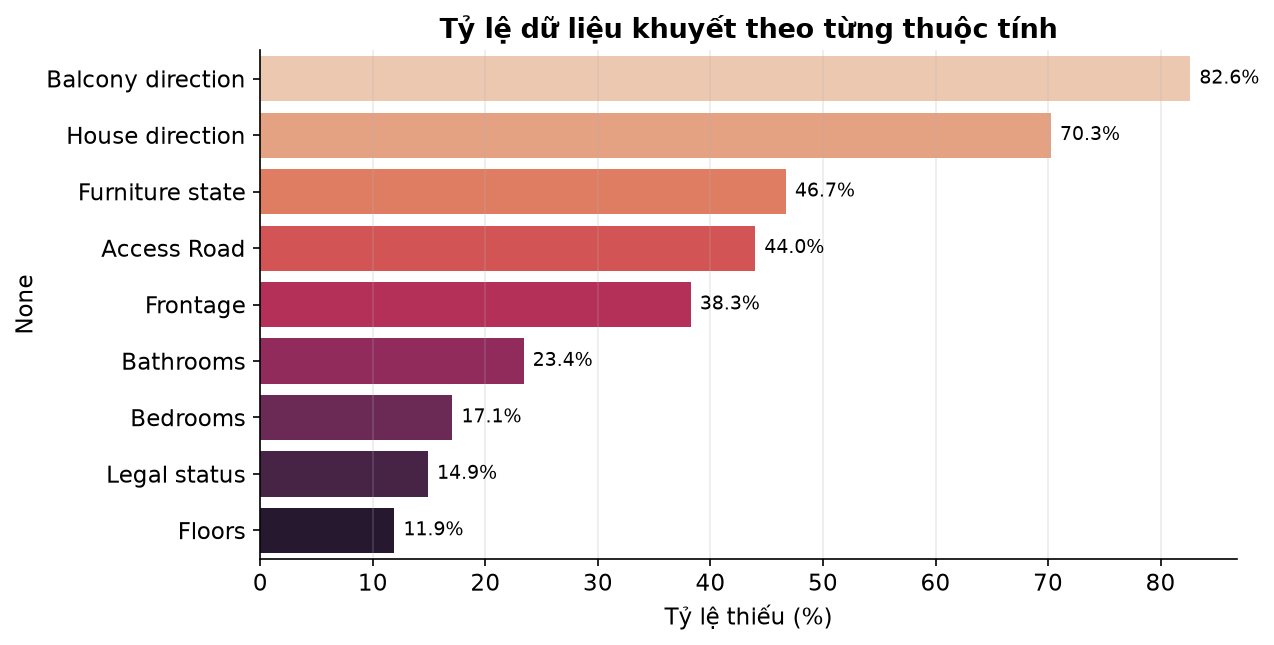
\includegraphics[width=0.86\textwidth]{hou_missing_ratio.png}
\caption[Tỷ lệ dữ liệu khuyết theo từng thuộc tính]%
{Tỷ lệ dữ liệu khuyết theo từng thuộc tính của tập bất động sản}
\label{fig:hou-missing}
\end{figure}

\bieudo{Biểu đồ cột ngang, sắp giảm dần theo tỷ lệ khuyết.}

\phanphoi{Trải rất rộng và liên tục --- từ $82{,}6\%$ xuống $11{,}9\%$, không có
khoảng đứt gãy rõ rệt giữa nhóm ``khuyết nhiều'' và nhóm ``khuyết ít''.}

\chitiet{\texttt{Balcony direction} đứng đầu với $82{,}6\%$ --- vượt ngưỡng loại
bỏ $80\%$ nên cột này bị loại khỏi mô hình. \texttt{House direction} khuyết
$70{,}3\%$ nhưng vẫn dưới ngưỡng nên được giữ. Tiếp theo là
\texttt{Furniture state} $46{,}7\%$, \texttt{Access Road} $44{,}0\%$,
\texttt{Frontage} $38{,}3\%$, \texttt{Bathrooms} $23{,}4\%$,
\texttt{Bedrooms} $17{,}1\%$, \texttt{Legal status} $14{,}9\%$ và
\texttt{Floors} $11{,}9\%$. Ba cột \texttt{Address}, \texttt{Area} và
\texttt{Price} đầy đủ hoàn toàn.}

\nhanxet{Việc giữ lại \texttt{House direction} dù khuyết $70{,}3\%$ là một quyết
định có căn cứ: hướng nhà mang ý nghĩa phong thuỷ đáng kể trong định giá tại
Việt Nam, và với biến định danh thì bản thân trạng thái ``không rõ'' cũng là một
hạng mục có ý nghĩa --- tin đăng không khai hướng nhà có thể chính là tin đăng
mà hướng nhà không phải điểm mạnh.}

\subsection{Tách địa chỉ thành hai cấp hành chính}

Cột \texttt{Address} là chuỗi tự do. Bước làm sạch tách nó thành
\texttt{Province} và \texttt{District}. Dữ liệu thật để lại nhiều dạng viết khác
nhau của cùng một địa danh --- ``Hà Nội'', ``HN'', ``Quận Nam Từ Liêm'' xuất hiện
ở cấp tỉnh; ``Hồ Chí Minh giá 2tỷ380'' cho thấy người đăng tin gõ lẫn giá vào ô
địa chỉ. Hệ thống giữ nguyên các biến thể này thay vì hợp nhất thủ công, và xử
lý bằng cơ chế gộp hạng mục hiếm ở bước mã hoá (Mục~\ref{sec:bieudien-hou}).

\section{Phân tích khám phá dữ liệu}
\label{sec:eda-hou}

\subsection{Ba biến người mua thật sự cân nhắc}

\begin{figure}[H]
\centering
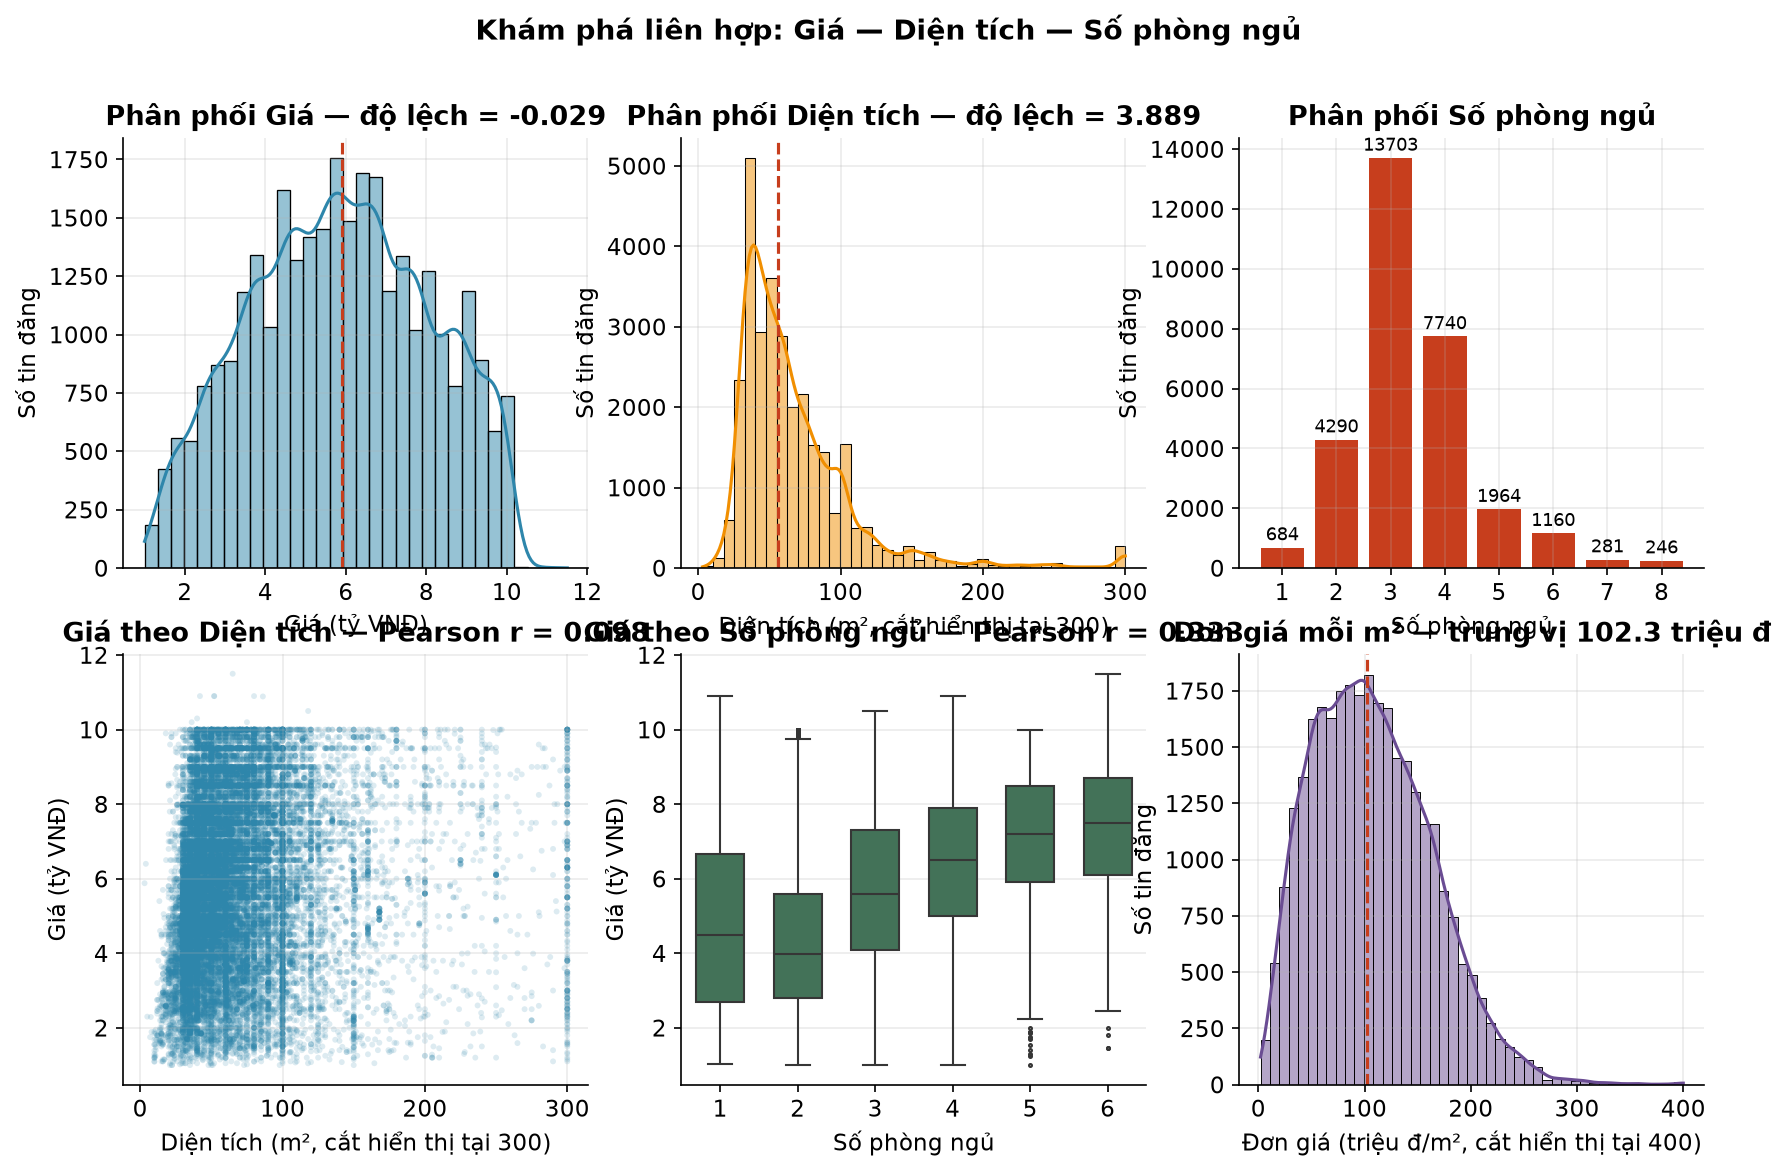
\includegraphics[width=\textwidth]{hou_price_area_bedrooms.png}
\caption[Khám phá liên hợp Giá -- Diện tích -- Số phòng ngủ]%
{Khám phá liên hợp Giá -- Diện tích -- Số phòng ngủ: ba phân phối biên ở hàng
trên, ba quan hệ chéo ở hàng dưới}
\label{fig:hou-joint}
\end{figure}

\bieudo{Lưới sáu bảng. Hàng trên là ba phân phối biên --- hai biểu đồ tần suất
kèm đường mật độ và một biểu đồ cột cho biến đếm. Hàng dưới là ba quan hệ ---
biểu đồ phân tán, biểu đồ hộp theo nhóm, và phân phối của một biến dẫn xuất.}

\phanphoi{Ba biến ở ba chế độ phân phối hoàn toàn khác nhau. \texttt{Price} gần
đối xứng, \texttt{Area} lệch phải rất mạnh, \texttt{Bedrooms} là biến đếm có một
đỉnh trội hẳn.}

\chitiet{\texttt{Price} có độ lệch $-0{,}029$ --- gần như đối xứng hoàn hảo ---
với trung vị $5{,}90$ tỷ. \texttt{Area} có độ lệch $3{,}889$, khối lượng dữ liệu
dồn trong khoảng $30$--$100$ m$^2$ với trung vị $56$ m$^2$, đuôi phải kéo tới
$595$ m$^2$. \texttt{Bedrooms} có đỉnh áp đảo tại 3 phòng ($13.703$ tin,
$45{,}3\%$), kế đến 4 phòng ($7.740$) và 2 phòng ($4.290$).

Hàng dưới cho ba con số quan trọng: Giá theo Diện tích có $r=0{,}098$; Giá theo
Số phòng ngủ có $r=0{,}333$ với các hộp chồng lấn rất nhiều; và đơn giá mỗi mét
vuông có độ lệch $2{,}135$ với trung vị $102{,}3$ triệu đồng/m$^2$.}

\begin{phathien}{Ba điều đi ngược trực giác, đọc được từ một hình}
\textbf{(1) Không được biến đổi log cho \texttt{Price} ở tập này.} Phép biến đổi
log là thao tác mặc định khi làm việc với giá nhà, vì giá nhà thị trường lệch
phải mạnh. Nhưng \texttt{Price} ở đây gần đối xứng ($-0{,}029$), nên lấy log sẽ
\emph{tạo ra} độ lệch trái thay vì sửa chữa gì. Giả định phải được đo trước khi
viện dẫn --- xem thêm Mục~\ref{sec:price-cat-bien}.

\textbf{(2) Diện tích gần như không định giá được căn nhà.} Hệ số $0{,}098$ có
nghĩa Diện tích một mình giải thích chưa tới $1\%$ phương sai của giá. Điều này
nghe vô lý cho tới khi nhớ rằng dữ liệu trải khắp cả nước: $56$ m$^2$ ở Cầu Giấy
và $56$ m$^2$ ở Phổ Yên là hai mức giá hoàn toàn khác nhau. Diện tích chỉ có ý
nghĩa \emph{sau khi đã cố định vị trí}.

\textbf{(3) Đơn giá mỗi m$^2$ mới là biến giữ đúng hình dáng mà trực giác mong
đợi} --- lệch phải mạnh với độ lệch $2{,}135$. Đây chính là biến bị \emph{ẩn} đi
khi chỉ nhìn Giá và Diện tích một cách tách rời, và là lời giải thích trực quan
cho việc vì sao \texttt{District} chi phối mô hình tới vậy
(Mục~\ref{sec:importance-hou}).
\end{phathien}

\subsection{Phân phối biến mục tiêu}

\begin{figure}[H]
\centering
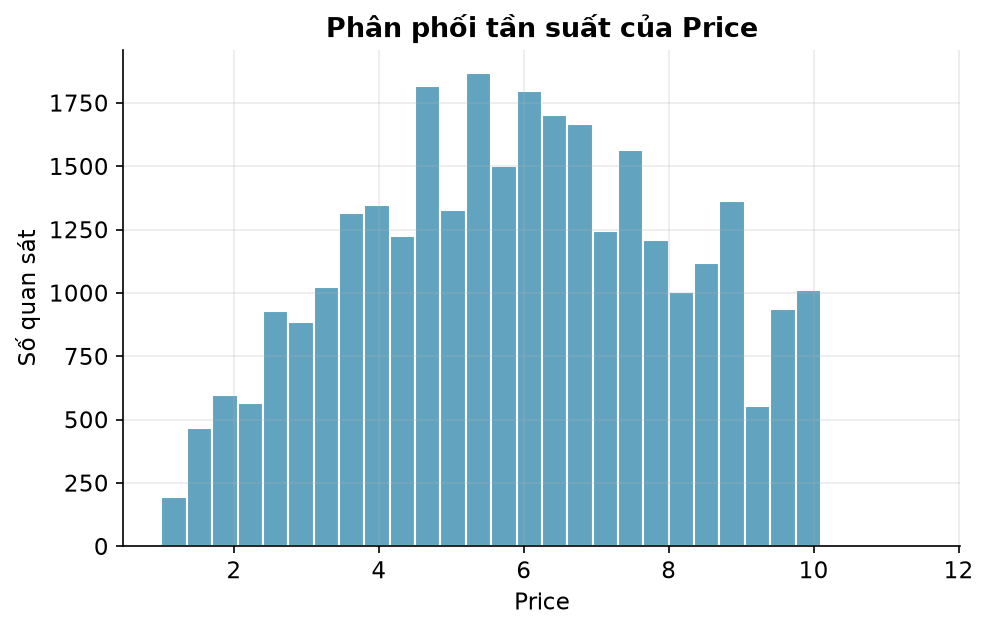
\includegraphics[width=0.82\textwidth]{hou_hist_price.png}
\caption[Phân phối tần suất của biến mục tiêu \texttt{Price}]%
{Phân phối tần suất của biến mục tiêu \texttt{Price}}
\label{fig:hou-hist-price}
\end{figure}

\bieudo{Biểu đồ tần suất, 30 khoảng.}

\phanphoi{Gần đối xứng, một đỉnh rộng và bằng phẳng ở giữa, hai đuôi cắt cụt đột
ngột ở cả hai đầu.}

\chitiet{Dữ liệu nằm gọn trong dải $1{,}0$ -- $11{,}5$ tỷ VNĐ, không có một quan
sát nào ngoài dải ấy. Đỉnh trải rộng trong khoảng $4$--$6$ tỷ với chiều cao
$1.700$--$1.870$ tin mỗi khoảng. Hai đầu dừng đột ngột chứ không thoải dần ---
dấu hiệu đặc trưng của dữ liệu đã bị cắt biên.}

\begin{phathien}{\texttt{Price} đã bị cắt biên từ nguồn --- và hệ quả không nhỏ}
\label{sec:price-cat-bien}
Thống kê đầy đủ: nhỏ nhất $1{,}00$, lớn nhất $11{,}50$, trung bình $5{,}8721$,
trung vị $5{,}90$, độ lệch chuẩn $2{,}2119$, độ lệch (skewness) $-0{,}029$, độ
nhọn (kurtosis) $-0{,}8464$. Trung bình xấp xỉ trung vị và độ lệch xấp xỉ $0$ ---
một phân phối gần đối xứng, gần như đều ở phần giữa.

Đây \textbf{không} phải hình dáng của giá bất động sản thật, vốn lệch phải rất
mạnh với một đuôi dài các bất động sản siêu cao cấp. Kết luận: người thu thập dữ
liệu đã lọc bỏ hai đầu trước khi công bố.

Hai hệ quả phải nói rõ:

\begin{enumerate}
  \item \textbf{$R^2$ ở đây khắt khe hơn bình thường.} Mẫu số
        của~\eqref{eq:r2} là phương sai của \texttt{Price}, và phương sai ấy đã
        bị thu hẹp do cắt biên. Cùng một sai số tuyệt đối sẽ cho $R^2$ thấp hơn
        so với trên một tập trải rộng.
  \item \textbf{Hệ thống chỉ áp dụng được trong đúng dải $1$--$11{,}5$ tỷ.} Mô
        hình cây \emph{không ngoại suy} --- đưa vào một biệt thự $50$ tỷ, nó vẫn
        trả về một con số nằm trong dải đã thấy lúc huấn luyện, và con số ấy sai
        hoàn toàn mà không có cảnh báo nào.
\end{enumerate}

Giả định ``giá nhà lệch phải mạnh'' nghe hiển nhiên tới mức suýt trôi qua mà
không ai đo. Nó đúng với thị trường thật và \emph{sai} với tập dữ liệu này.
\end{phathien}

\subsection{Quan hệ giữa diện tích và giá}

\begin{figure}[H]
\centering
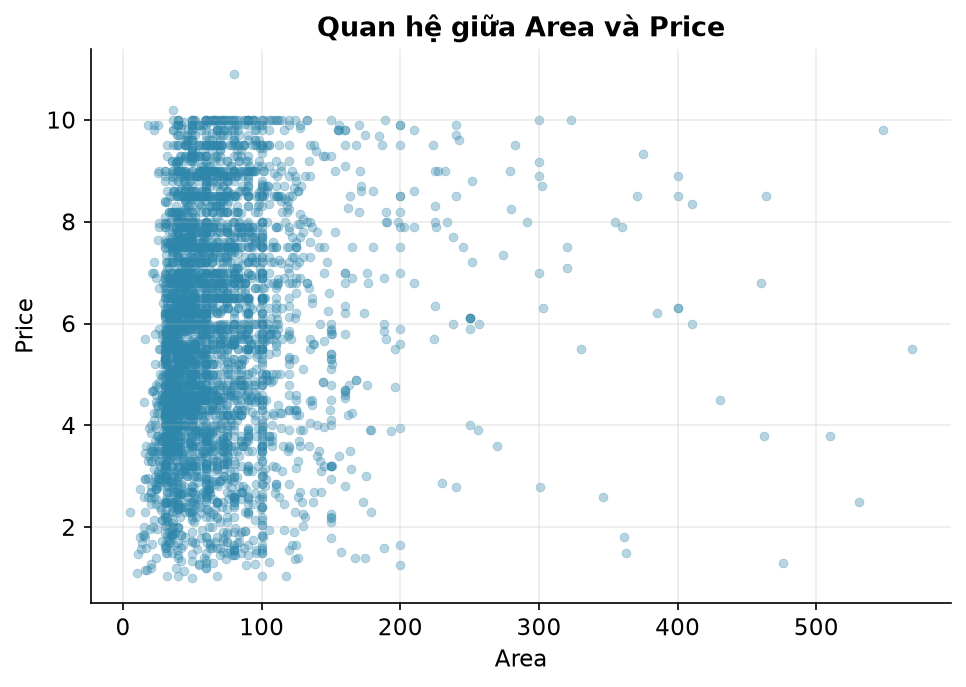
\includegraphics[width=0.82\textwidth]{hou_scatter_area_price.png}
\caption[Quan hệ giữa Diện tích và Giá]%
{Biểu đồ phân tán giữa Diện tích và Giá}
\label{fig:hou-scatter}
\end{figure}

\bieudo{Biểu đồ phân tán (scatter plot) với độ trong suốt cao để thấy mật độ
điểm ở vùng chồng chất.}

\phanphoi{Đám mây điểm dày đặc ở góc trái, thưa dần rất nhanh về phía phải; theo
trục dọc thì trải gần như đều khắp dải giá.}

\chitiet{Với diện tích dưới $130$ m$^2$, giá trải gần như kín toàn bộ dải
$1$--$11{,}5$ tỷ --- cùng một mức diện tích ứng với mọi mức giá. Từ $150$ m$^2$
trở lên điểm thưa hẳn nhưng vẫn không hình thành xu hướng đi lên rõ rệt: có căn
$400$ m$^2$ giá $3{,}8$ tỷ nằm cạnh căn $80$ m$^2$ giá $10$ tỷ. Đường giới hạn
trên ở mức $10$--$11{,}5$ tỷ hiện ra thành một vệt ngang --- chính là biên cắt
đã nêu.}

\subsection{Vị trí hành chính và tình trạng pháp lý}

\begin{figure}[H]
\centering
\begin{subfigure}[b]{0.52\textwidth}
  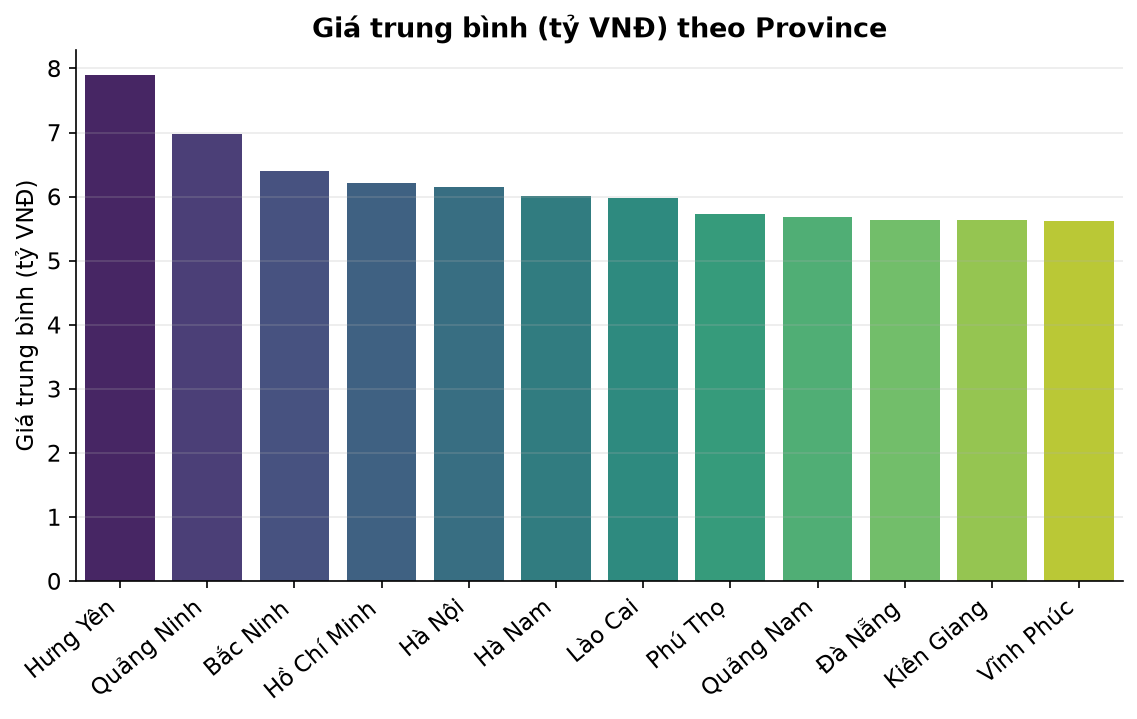
\includegraphics[width=\textwidth]{hou_bar_province.png}
  \caption{Giá trung bình theo Tỉnh/Thành}
  \label{fig:hou-bar-province}
\end{subfigure}
\hfill
\begin{subfigure}[b]{0.45\textwidth}
  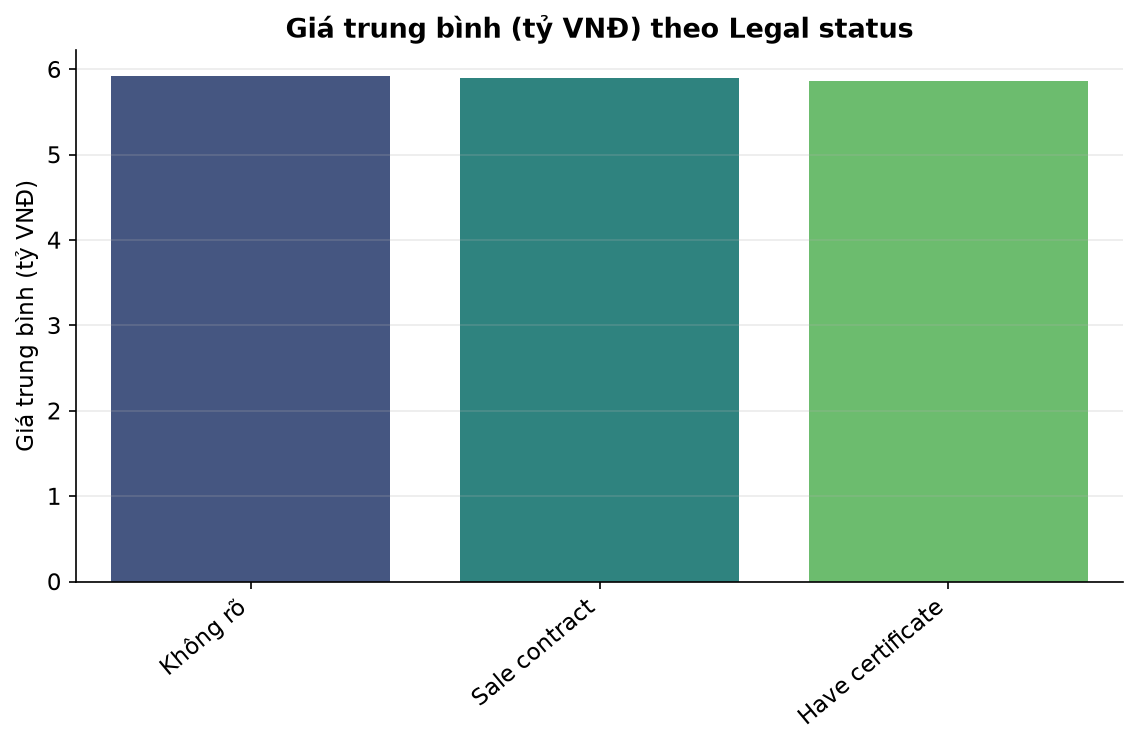
\includegraphics[width=\textwidth]{hou_bar_legal.png}
  \caption{Giá trung bình theo Tình trạng pháp lý}
  \label{fig:hou-bar-legal}
\end{subfigure}
\caption[Giá trung bình theo hai biến định danh]%
{Giá trung bình theo Tỉnh/Thành (12 tỉnh dẫn đầu) và theo Tình trạng pháp lý}
\label{fig:hou-bars}
\end{figure}

\bieudo{Hai biểu đồ cột đứng, mỗi cột là giá trung bình của một hạng mục.}

\phanphoi{Hai hình cho hai câu chuyện trái ngược. Bảng bên trái có độ dốc rõ; bảng
bên phải gần như phẳng hoàn toàn.}

\chitiet{Theo tỉnh, dẫn đầu là Hưng Yên $7{,}895$ tỷ (404 tin), rồi Quảng Ninh
$6{,}984$ (110 tin), Bắc Ninh $6{,}402$ (167 tin), Hồ Chí Minh $6{,}214$
(11.778 tin) và Hà Nội $6{,}154$ (10.457 tin). Chênh lệch giữa đầu và cuối bảng
là khoảng $2{,}3$ tỷ.

Theo pháp lý, ba hạng mục gần như bằng nhau: ``Không rõ'' $5{,}9263$,
``Sale contract'' $5{,}8933$, ``Have certificate'' $5{,}8614$ --- chênh lệch chỉ
$0{,}065$ tỷ, tức $1{,}1\%$.}

\begin{phathien}{Trung bình biên che mất cấu trúc có điều kiện}
Hai hình trên gợi ý rằng pháp lý không ảnh hưởng tới giá, và rằng Hưng Yên là
tỉnh đắt nhất Việt Nam. Cả hai kết luận đều sai, và sai vì cùng một lý do:
\emph{trung bình biên trộn lẫn mọi điều kiện khác}.

Hưng Yên đứng đầu không phải vì đất Hưng Yên đắt hơn đất Quận 1, mà vì 404 tin
đăng ở đó tình cờ là các dự án lớn; trong khi trung bình của Hồ Chí Minh bị kéo
xuống bởi hàng nghìn căn nhỏ ở vùng ven. Tương tự, giấy tờ đầy đủ có giá trị
thật, nhưng những căn thiếu giấy tờ trong tập này lại tập trung ở phân khúc cao
hơn, và hai hiệu ứng triệt tiêu nhau khi lấy trung bình.

Mô hình cây \emph{không} bị đánh lừa như vậy vì nó học quan hệ \emph{có điều
kiện}: sau khi đã chia theo quận, nó mới xét tới pháp lý. Bằng chứng là
\texttt{Legal status} vẫn nhận mức quan trọng $0{,}0133$ ở
Mục~\ref{sec:importance-hou} --- nhỏ, nhưng khác $0$ rõ rệt.
\end{phathien}

\subsection{Ma trận tương quan}

\begin{figure}[H]
\centering
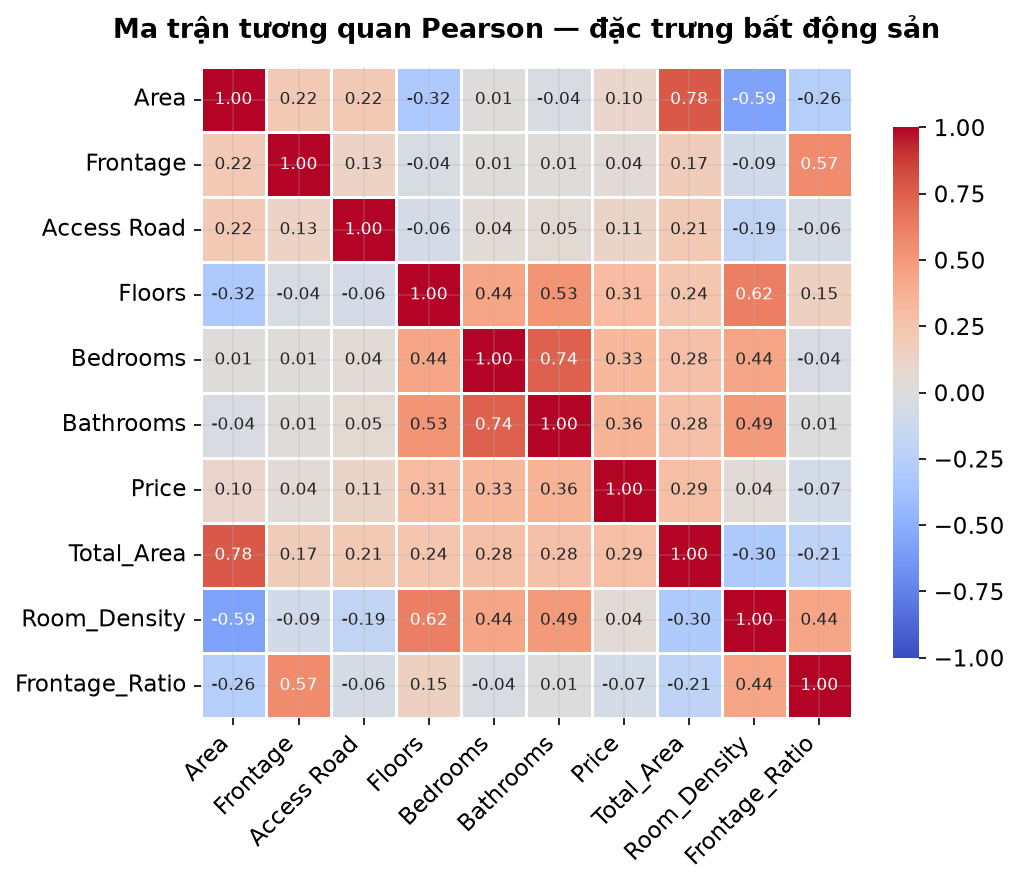
\includegraphics[width=0.94\textwidth]{hou_corr_heatmap.png}
\caption[Ma trận tương quan Pearson của các đặc trưng bất động sản]%
{Ma trận tương quan Pearson của các đặc trưng bất động sản}
\label{fig:hou-corr}
\end{figure}

\bieudo{Bản đồ nhiệt đối xứng, thang màu hai chiều từ xanh (âm) qua trắng (không
tương quan) tới đỏ (dương).}

\phanphoi{Khác hẳn ma trận ở Hình~\ref{fig:dia-corr}: ở đây có cả tương quan âm
rõ rệt, và cột \texttt{Price} thì nhạt màu gần như toàn bộ.}

\chitiet{Cặp mạnh nhất là \texttt{Area}--\texttt{Total\_Area} $=0{,}78$ (đúng
theo định nghĩa) và \texttt{Bedrooms}--\texttt{Bathrooms} $=0{,}74$. Có ba tương
quan âm đáng kể: \texttt{Area}--\texttt{Room\_Density} $=-0{,}59$,
\texttt{Area}--\texttt{Floors} $=-0{,}32$ và \texttt{Area}--\texttt{Frontage\_Ratio}
$=-0{,}26$. Với \texttt{Price}, hệ số cao nhất chỉ là $0{,}364$
(\texttt{Bathrooms}), rồi $0{,}333$ (\texttt{Bedrooms}), $0{,}309$
(\texttt{Floors}), $0{,}290$ (\texttt{Total\_Area}) và $0{,}098$
(\texttt{Area}).}

\begin{phathien}{Trần của mô hình tuyến tính đọc được ngay từ ma trận tương quan}
Không đặc trưng định lượng nào tương quan tuyến tính với giá quá $0{,}364$.
Với một mô hình tuyến tính, $R^2$ tối đa đạt được bị chặn bởi chính các hệ số
này --- và Linear Regression thực tế đạt $R^2 = 0{,}3557$
(Bảng~\ref{tab:ketqua-hou}), gần khít với dự đoán.

Đây là một kiểm chứng đẹp: ma trận tương quan tính được \emph{trước khi} huấn
luyện bất kỳ mô hình nào đã báo trước đúng trần hiệu năng của cả một họ thuật
toán. Nó cũng nói luôn rằng muốn vượt trần ấy thì phải đưa vào thông tin mà các
cột định lượng không chứa --- tức là các biến định danh về vị trí, đúng như Thực
nghiệm~3 sẽ đo được ở Mục~\ref{sec:tn3-hou}.

Quan hệ âm \texttt{Area}--\texttt{Floors} $=-0{,}32$ cũng nói một điều thật về
đô thị Việt Nam: nhà mặt đất diện tích nhỏ thì xây cao lên, còn nhà diện tích
lớn thường là nhà vườn hoặc biệt thự thấp tầng.
\end{phathien}

\section{Thiết kế đặc trưng và biểu diễn}
\label{sec:bieudien-hou}

\begin{table}[H]
\centering
\caption{Ba đặc trưng thiết kế cho bài toán bất động sản}
\label{tab:engineered-hou}
\small
\begin{tabularx}{\textwidth}{@{}L{2.9cm}L{4.4cm}X@{}}
\toprule
\textbf{Đặc trưng} & \textbf{Công thức} & \textbf{Căn cứ} \\
\midrule
\texttt{Total\_Area}     & $\texttt{Area}\times\max(\texttt{Floors},1)$ & Tổng diện tích sàn sử dụng, thứ người mua thật sự trả tiền \\
\addlinespace
\texttt{Room\_Density}   & $\dfrac{\texttt{Bedrooms}+\texttt{Bathrooms}}{\max(\texttt{Area},1)}$ & Mật độ phòng --- phân biệt nhà ở gia đình với nhà chia phòng cho thuê \\
\addlinespace
\texttt{Frontage\_Ratio} & $\dfrac{\texttt{Frontage}}{\max(\texttt{Area},1)}$ & Tỷ lệ mặt tiền --- đại lượng quyết định khả năng kinh doanh \\
\bottomrule
\end{tabularx}
\end{table}

Năm biến định danh được mã hoá one-hot với giới hạn 30 hạng mục phổ biến nhất
mỗi biến; các hạng mục hiếm gộp chung vào một nhóm. Không có giới hạn này,
riêng \texttt{District} với hàng trăm giá trị sẽ tạo ma trận thưa khổng lồ và
khiến mô hình học thuộc từng quận hiếm thay vì học quy luật giá. Kết quả:
biểu diễn cuối cùng có \textbf{84 chiều} từ 14 cột ban đầu.

\begin{table}[H]
\centering
\caption{Kích thước ba tập dữ liệu và kết quả mô hình cơ sở}
\label{tab:split-hou}
\small
\begin{tabular}{@{}lrr@{\hspace{1.4cm}}lr@{}}
\toprule
\textbf{Tập} & \textbf{Số tin} & \textbf{Tỷ lệ} & \textbf{Mô hình cơ sở} & \textbf{Giá trị} \\
\midrule
Huấn luyện & 21.764 & 72{,}0\% & MAE  & 1{,}8587 \\
Kiểm tra   &  5.442 & 18{,}0\% & RMSE & 2{,}2265 \\
Ngoại kiểm &  3.023 & 10{,}0\% & $R^2$ & \textbf{$-0{,}0008$} \\
\textbf{Tổng} & \textbf{30.229} & \textbf{100\%} & & \\
\bottomrule
\end{tabular}
\end{table}

\nhanxet{MAE $=1{,}8587$ của mô hình cơ sở đọc thẳng ra tiền: không dùng mô hình
nào thì sai số trung bình khi định giá một căn nhà là gần \textbf{1,86 tỷ VNĐ}.
$R^2 = -0{,}0008$ xấp xỉ $0$ đúng như lý thuyết --- đoán trung vị không giải
thích được chút phương sai nào.}

\section{Thực nghiệm 1 --- Đối đầu năm mô hình}
\label{sec:tn1-hou}

\begin{table}[H]
\centering
\caption{Kết quả năm mô hình hồi quy trên tập kiểm tra, sắp theo $R^2$}
\label{tab:ketqua-hou}
\small
\begin{tabular}{@{}lrrrr@{}}
\toprule
\textbf{Mô hình} & \textbf{MAE} & \textbf{MSE} & \textbf{RMSE} & \textbf{$R^2$} \\
\midrule
Mô hình cơ sở (trung vị)  & 1{,}8587 & 4{,}9573 & 2{,}2265 & $-0{,}0008$ \\
\midrule
XGBoost                   & \textbf{1{,}0493} & \textbf{1{,}9115} & \textbf{1{,}3826} & \textbf{0{,}6141} \\
Random Forest             & 1{,}0818 & 2{,}0184 & 1{,}4207 & 0{,}5925 \\
Support Vector Regression & 1{,}0743 & 2{,}0883 & 1{,}4451 & 0{,}5784 \\
Decision Tree             & 1{,}2412 & 2{,}7519 & 1{,}6589 & 0{,}4444 \\
Linear Regression         & 1{,}2677 & 3{,}1914 & 1{,}7865 & 0{,}3557 \\
\bottomrule
\end{tabular}
\end{table}

\begin{figure}[H]
\centering
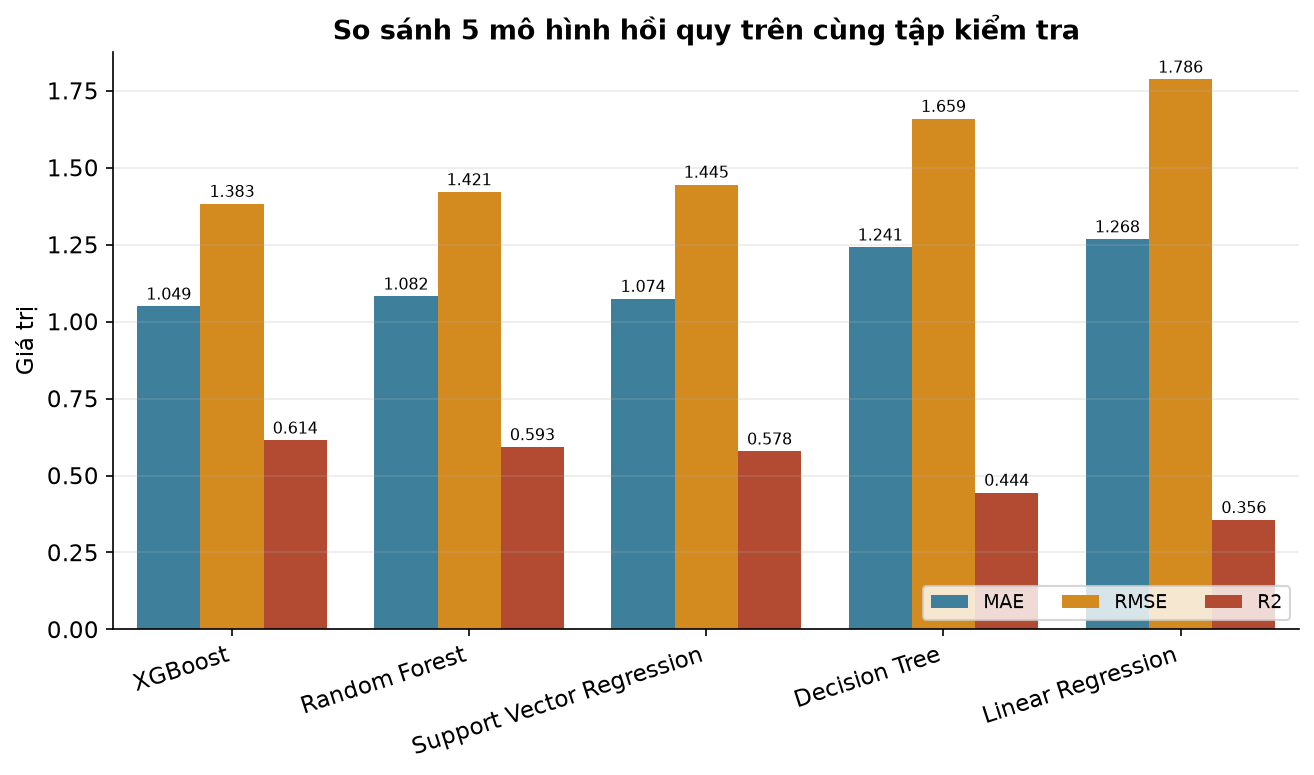
\includegraphics[width=\textwidth]{hou_model_comparison.png}
\caption[So sánh năm mô hình hồi quy trên ba độ đo]%
{So sánh năm mô hình hồi quy trên cùng tập kiểm tra}
\label{fig:hou-comparison}
\end{figure}

\nhanxet{Thứ hạng ở đây \textbf{ngược hẳn} với bài toán tiểu đường. Hai mô hình
tổ hợp phức tạp nhất --- XGBoost và Random Forest --- đứng đầu, còn mô hình
tuyến tính đơn giản nhất đứng cuối. Lời giải thích nằm ở quy mô dữ liệu và cấu
trúc quan hệ:

\begin{itemize}
  \item \textbf{21.764 mẫu huấn luyện} so với 552 ở bài toán tiểu đường --- gấp
        gần 40 lần. Mô hình phương sai cao giờ có đủ dữ liệu để phát huy.
  \item \textbf{Quan hệ giá là phi tuyến và có tương tác mạnh}: hiệu ứng của
        diện tích phụ thuộc hoàn toàn vào quận. Cây quyết định biểu diễn được
        tương tác này một cách tự nhiên; mô hình tuyến tính thì không, và trần
        của nó đã được ma trận tương quan báo trước.
\end{itemize}

Bài học phương pháp: \emph{không có thuật toán nào tốt nhất một cách tuyệt
đối}. Cùng một bộ năm thuật toán, chạy trên hai bài toán, cho hai thứ hạng gần
như đảo ngược. Đây là lý do phải chạy đối đầu thay vì chọn theo danh tiếng.}

\subsection{Giá dự đoán so với giá thật}

\begin{figure}[H]
\centering
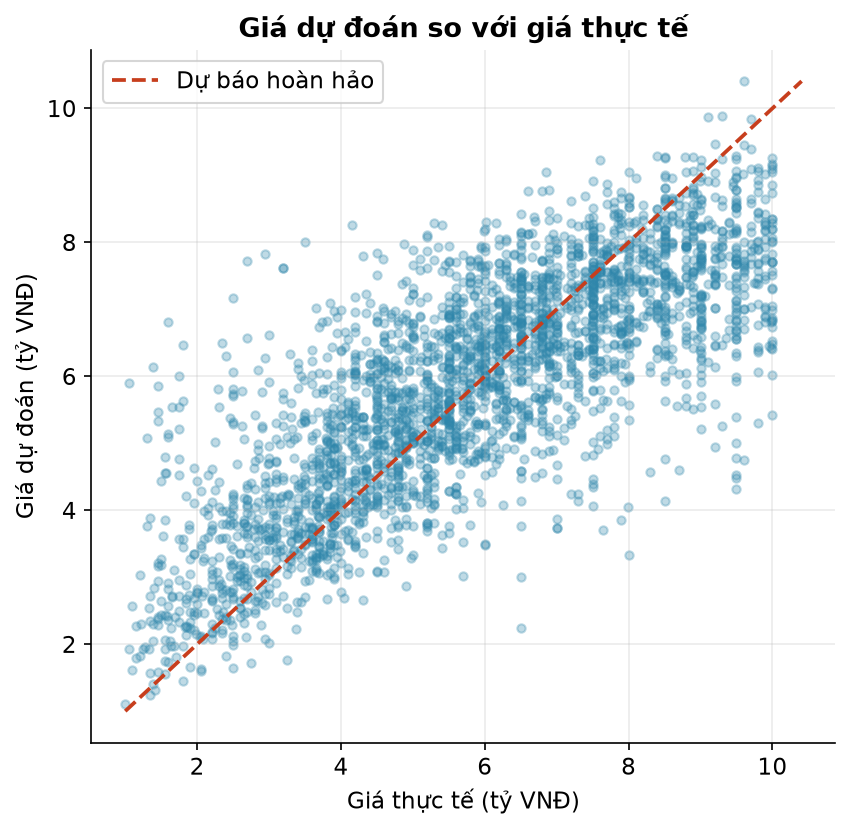
\includegraphics[width=0.82\textwidth]{hou_pred_vs_true.png}
\caption[Giá dự đoán so với giá thật của mô hình XGBoost]%
{Giá dự đoán so với giá thật của mô hình XGBoost trên tập kiểm tra}
\label{fig:hou-pred-true}
\end{figure}

\bieudo{Biểu đồ phân tán dự báo -- thực tế, kèm đường chéo tham chiếu ứng với dự
báo hoàn hảo.}

\phanphoi{Đám mây điểm bám quanh đường chéo nhưng \textbf{thoải hơn} đường chéo:
ở vùng giá thấp nó nằm phía trên, ở vùng giá cao nó nằm phía dưới.}

\chitiet{Trong khoảng $4$--$7$ tỷ, đám mây bám sát đường chéo và tương đối hẹp.
Từ $8$ tỷ trở lên, gần như toàn bộ điểm rơi xuống dưới đường chéo --- mô hình
định giá hụt. Ở phía dưới $3$ tỷ thì ngược lại, điểm nằm trên đường chéo. Hình
dáng ``chữ S nằm'' này là dấu hiệu kinh điển của hồi quy về trung bình.}

\subsection{Phân tích phần dư}
\label{sec:chech-hou}

\begin{figure}[H]
\centering
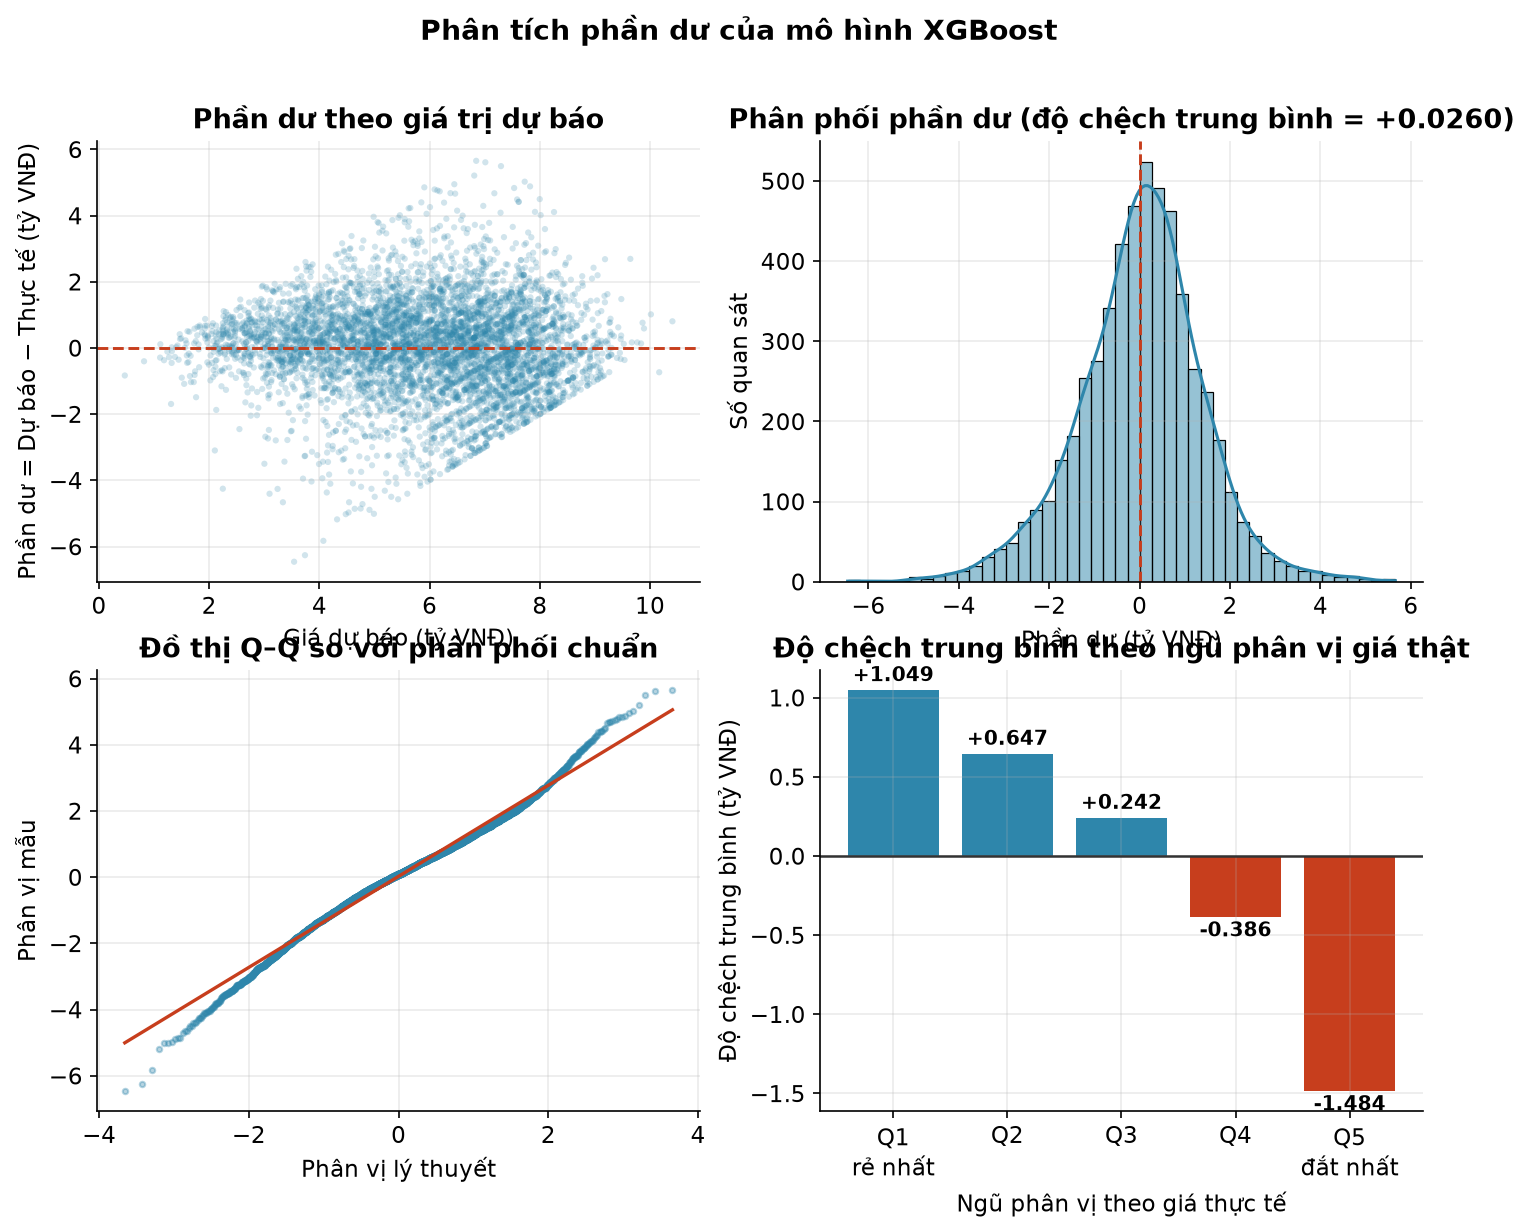
\includegraphics[width=\textwidth]{hou_residual_analysis.png}
\caption[Phân tích phần dư của mô hình XGBoost]%
{Phân tích phần dư của mô hình XGBoost --- bốn góc nhìn về cách mô hình sai}
\label{fig:hou-residual}
\end{figure}

\bieudo{Lưới bốn bảng: biểu đồ phân tán phần dư, biểu đồ tần suất phần dư, đồ
thị Q--Q so với phân phối chuẩn, và biểu đồ cột độ chệch theo ngũ phân vị.}

\phanphoi{Ba bảng đầu trông tương đối lành mạnh --- phần dư tập trung quanh $0$,
gần đối xứng. Bảng thứ tư phá vỡ ấn tượng ấy: các cột không dao động ngẫu nhiên
quanh $0$ mà \textbf{giảm đơn điệu} từ dương sang âm.}

\chitiet{Bảng 1: đám mây phần dư nghiêng rõ rệt, dày ở vùng dự báo $4$--$7$ tỷ.
Bảng 2: phân phối phần dư gần đối xứng quanh $0$ với hai đuôi tương đương. Bảng
3: Q--Q bám đường chuẩn ở phần giữa nhưng lệch ở hai đuôi --- phần dư có đuôi
dày hơn phân phối chuẩn. Bảng 4 là bảng quyết định, chi tiết ở
Bảng~\ref{tab:chech-hou}.}

\begin{table}[H]
\centering
\caption{Độ chệch và MAE theo ngũ phân vị giá thật, mô hình XGBoost}
\label{tab:chech-hou}
\small
\begin{tabular}{@{}lrrrrr@{}}
\toprule
\textbf{Ngũ phân vị} & \textbf{Số tin} & \textbf{Giá thật TB} & \textbf{Giá dự báo TB} & \textbf{Độ chệch} & \textbf{MAE} \\
\midrule
Q1 --- rẻ nhất & 1.089 & 2{,}6849 & 3{,}7338 & \textbf{$+1{,}0488$} & 1{,}1575 \\
Q2             & 1.114 & 4{,}5032 & 5{,}1497 & $+0{,}6465$ & 0{,}9366 \\
Q3 --- giữa    & 1.133 & 5{,}9186 & 6{,}1605 & $+0{,}2419$ & \textbf{0{,}7889} \\
Q4             & 1.030 & 7{,}2372 & 6{,}8511 & $-0{,}3860$ & 0{,}8375 \\
Q5 --- đắt nhất& 1.076 & 8{,}9774 & 7{,}4930 & \textbf{$-1{,}4844$} & \textbf{1{,}5335} \\
\bottomrule
\end{tabular}
\end{table}

\begin{phathien}{Độ chệch đơn điệu theo phân khúc --- phát hiện phải nói với người dùng}
Độ chệch không dao động ngẫu nhiên mà giảm đều từ $+1{,}0488$ xuống $-1{,}4844$
qua năm ngũ phân vị. Hai nguyên nhân cộng dồn:

\begin{enumerate}
  \item \textbf{Hồi quy về trung bình~\cite{hastie2009}.} Cực tiểu hoá MSE ở~\eqref{eq:mse} kéo
        mọi dự báo về phía trung tâm phân phối, vì sai lớn bị phạt bình phương.
  \item \textbf{Mô hình cây không ngoại suy.} Giá trị dự báo của một cây là
        trung bình các mẫu huấn luyện trong lá, nên nó không bao giờ vượt quá
        khoảng giá trị đã thấy.
\end{enumerate}

MAE cũng không đều: $0{,}7889$ ở nhóm giữa nhưng $1{,}5335$ ở nhóm đắt nhất ---
gần gấp đôi. Con số MAE gộp $1{,}0493$ là trung bình của hai chế độ sai rất khác
nhau, và nó \emph{che mất} điều đó.

\textbf{Hệ quả bắt buộc phải hiển thị cho người dùng:} với bất động sản cao cấp,
con số hệ thống đưa ra là \textbf{cận dưới}, không phải ước lượng không chệch.
Một hệ thống định giá im lặng về điều này sẽ khiến người bán nhà cao cấp bị
thiệt một cách có hệ thống.
\end{phathien}

\section{Thực nghiệm 2 --- Khảo sát độ sâu của rừng ngẫu nhiên}
\label{sec:tn2-hou}

\begin{figure}[H]
\centering
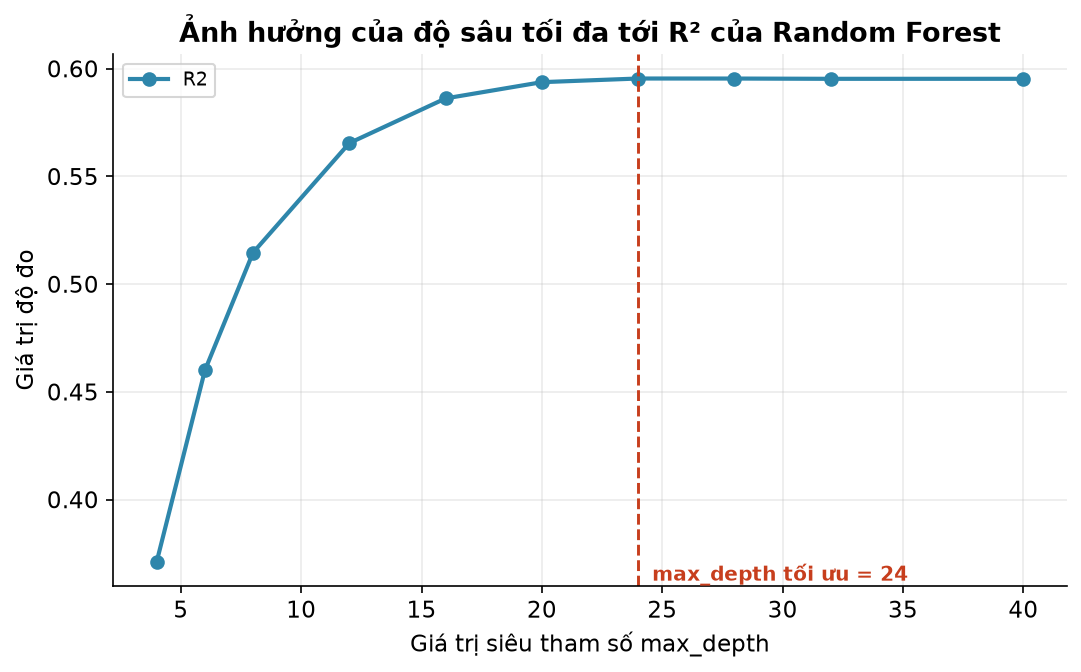
\includegraphics[width=0.88\textwidth]{hou_depth_sweep.png}
\caption[Ảnh hưởng của độ sâu tối đa tới $R^2$ của Random Forest]%
{Ảnh hưởng của độ sâu tối đa tới $R^2$ của Random Forest}
\label{fig:hou-depth}
\end{figure}

\bieudo{Biểu đồ đường. Trục ngang là \texttt{max\_depth}, trục dọc là $R^2$.}

\phanphoi{Dạng bão hoà cổ điển: tăng nhanh ở đầu dải, chậm dần, rồi đi ngang
hoàn toàn --- không có đoạn đi xuống, tức không thấy dấu hiệu học thuộc.}

\chitiet{$R^2$ tăng từ $0{,}3712$ ở độ sâu $4$ lên $0{,}5654$ ở độ sâu $12$ ---
phần lớn mức cải thiện nằm ở đoạn này. Từ $16$ tới $20$ chỉ còn tăng nhẹ
($0{,}5862 \to 0{,}5937$), rồi đạt đỉnh $0{,}5954$ tại độ sâu $24$. Từ $28$ trở
đi đường cong bằng phẳng tuyệt đối: $0{,}5954$, $0{,}5953$, $0{,}5953$.}

\begin{table}[H]
\centering
\caption{Khảo sát độ sâu tối đa --- kết quả đầy đủ}
\label{tab:depth-hou}
\small
\begin{tabular}{@{}rrrr@{}}
\toprule
\textbf{max\_depth} & \textbf{MAE} & \textbf{RMSE} & \textbf{$R^2$} \\
\midrule
4  & 1{,}4240 & 1{,}7648 & 0{,}3712 \\
8  & 1{,}2275 & 1{,}5506 & 0{,}5146 \\
12 & 1{,}1376 & 1{,}4671 & 0{,}5654 \\
16 & 1{,}0947 & 1{,}4317 & 0{,}5862 \\
20 & 1{,}0774 & 1{,}4186 & 0{,}5937 \\
\textbf{24} & 1{,}0716 & 1{,}4156 & \textbf{0{,}5954} \\
28 & 1{,}0704 & 1{,}4157 & 0{,}5954 \\
40 & 1{,}0703 & 1{,}4159 & 0{,}5953 \\
\bottomrule
\end{tabular}
\end{table}

\nhanxet{Bẫy ``cực trị chạm biên'' xuất hiện lần thứ hai trong dự án này. Dải
khảo sát ban đầu dừng ở $24$ và $R^2$ đạt đỉnh đúng tại đầu mút. Chỉ sau khi nới
dải tới $40$ mới xác nhận được rằng đó là đỉnh thật chứ không phải điểm cắt cụt.

Việc đường cong \emph{không} đi xuống ở độ sâu lớn là nhờ
\texttt{min\_samples\_leaf=5}: tham số này chặn cây mọc tới lá chỉ chứa một quan
sát. Nó còn có tác dụng phụ quan trọng về kỹ thuật --- để mặc định, rừng 200 cây
trên 21.764 dòng chiếm $156$ MB trên đĩa và vượt giới hạn $100$ MB mỗi tệp của
GitHub. Đặt bằng $5$ thì còn $44$ MB mà $R^2$ chỉ giảm từ $0{,}5976$ xuống
$0{,}5925$.}

\section{Thực nghiệm 3 --- Ảnh hưởng của cách biểu diễn dữ liệu}
\label{sec:tn3-hou}

\textbf{Thiết kế.} Ba phương án biểu diễn, cùng chạy trên Random Forest độ sâu
$16$, cùng phép chia dữ liệu.

\begin{table}[H]
\centering
\caption{Ba phương án biểu diễn và kết quả trên Random Forest}
\label{tab:rep-hou}
\small
\begin{tabular}{@{}lrrrr@{}}
\toprule
\textbf{Phương án biểu diễn} & \textbf{MAE} & \textbf{MSE} & \textbf{RMSE} & \textbf{$R^2$} \\
\midrule
Định lượng $+$ định danh, chưa thiết kế & \textbf{1{,}0932} & \textbf{2{,}0294} & \textbf{1{,}4246} & \textbf{0{,}5903} \\
Đầy đủ $+$ đặc trưng thiết kế           & 1{,}0947 & 2{,}0497 & 1{,}4317 & 0{,}5862 \\
Chỉ đặc trưng định lượng                & 1{,}4388 & 3{,}2988 & 1{,}8163 & 0{,}3340 \\
\bottomrule
\end{tabular}
\end{table}

\begin{figure}[H]
\centering
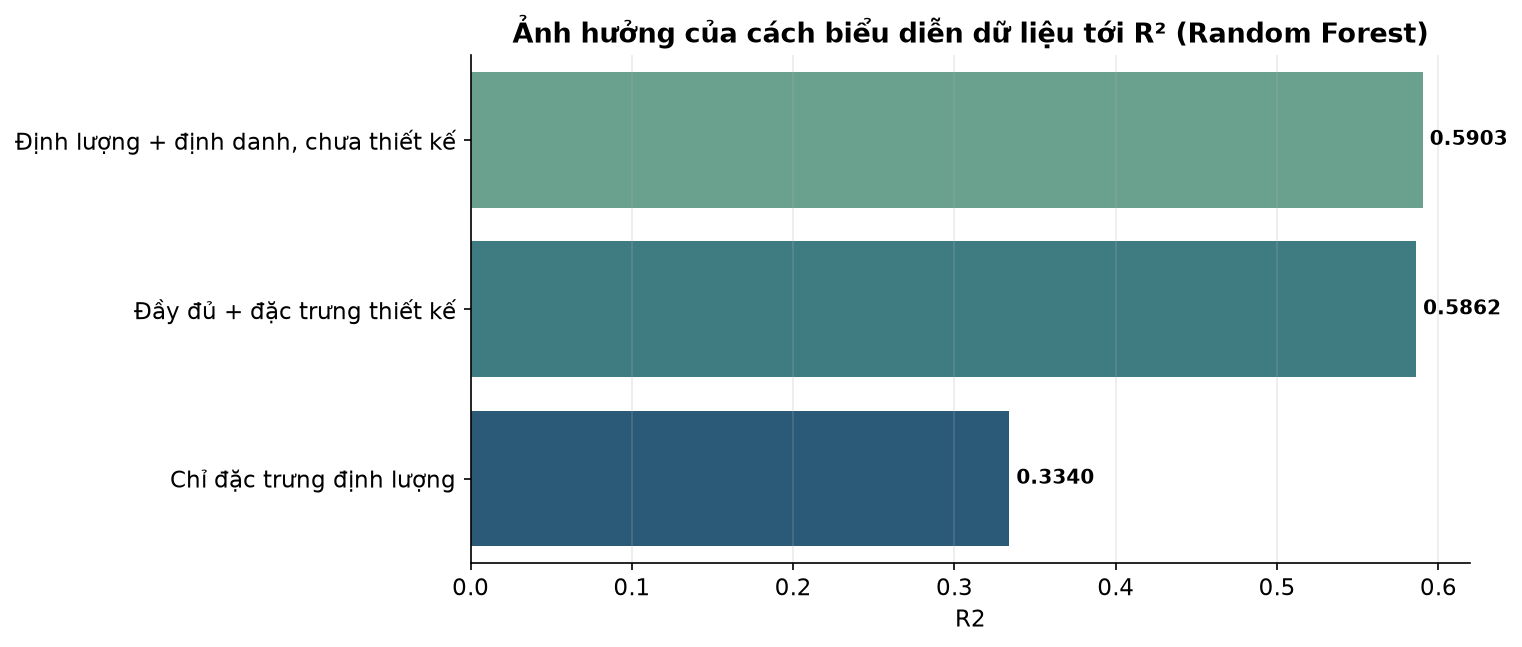
\includegraphics[width=\textwidth]{hou_representation.png}
\caption[Ảnh hưởng của cách biểu diễn dữ liệu tới $R^2$]%
{Ảnh hưởng của cách biểu diễn dữ liệu tới $R^2$ của Random Forest}
\label{fig:hou-representation}
\end{figure}

\bieudo{Biểu đồ cột ngang, sắp giảm dần theo $R^2$.}

\phanphoi{Hai cột đầu gần bằng nhau, cột thứ ba \emph{ngắn hơn hẳn} --- một
khoảng đứt gãy rõ rệt, khác hẳn hình dáng gần đều ở Hình~\ref{fig:dia-representation}.}

\chitiet{Hai phương án có biến định danh cho $R^2$ $0{,}5903$ và $0{,}5862$ ---
chênh nhau $0{,}0041$, tức trong nhiễu. Bỏ hết biến định danh làm $R^2$ tụt
xuống $0{,}3340$ --- mất $0{,}2563$, tức hơn $43\%$ năng lực giải thích. MAE
đồng thời xấu đi từ $1{,}0932$ lên $1{,}4388$ tỷ VNĐ.}

\begin{table}[H]
\centering
\caption{Biên độ do đổi biểu diễn so với biên độ do đổi thuật toán, bài toán bất động sản}
\label{tab:biendo-hou}
\small
\begin{tabular}{@{}lrl@{}}
\toprule
\textbf{Nguồn biến thiên} & \textbf{Biên độ $R^2$} & \textbf{Ghi chú} \\
\midrule
Đổi cách biểu diễn (3 phương án) & 0{,}2563 & $0{,}3340 \to 0{,}5903$ \\
Đổi thuật toán (5 mô hình)       & 0{,}2584 & $0{,}3557 \to 0{,}6141$ \\
\midrule
\textbf{Tỷ số} & \multicolumn{2}{l}{\textbf{Ngang bằng --- nhưng đổi biểu diễn ít công hơn nhiều}} \\
\bottomrule
\end{tabular}
\end{table}

\nhanxet{Hai kết luận, một trong đó đi ngược kỳ vọng ban đầu.

\textbf{(1) Vị trí hành chính là nhóm thông tin quyết định.} Đây là kết luận
mạnh nhất của cả chương, và nó nhất quán với ba bằng chứng độc lập: tương quan
tuyến tính yếu của mọi biến định lượng (Hình~\ref{fig:hou-corr}), mức quan trọng
đặc trưng (Mục~\ref{sec:importance-hou}), và thực nghiệm này.

\textbf{(2) Ba đặc trưng thiết kế \emph{không} giúp gì.} $R^2$ giảm nhẹ từ
$0{,}5903$ xuống $0{,}5862$ khi thêm chúng vào. Lý do giống hệt trường hợp
\texttt{Glucose\_Level} ở Mục~\ref{sec:importance-dia}: cây quyết định
\emph{tự} tìm được các tổ hợp cần thiết, nên cung cấp sẵn
$\texttt{Area}\times\texttt{Floors}$ chỉ thêm một cột tương quan $0{,}78$ với cột
đã có mà không thêm thông tin nào.}

\section{Thực nghiệm 4 --- Kiểm chuẩn ngoài phân phối}
\label{sec:tn4-hou}

\begin{figure}[H]
\centering
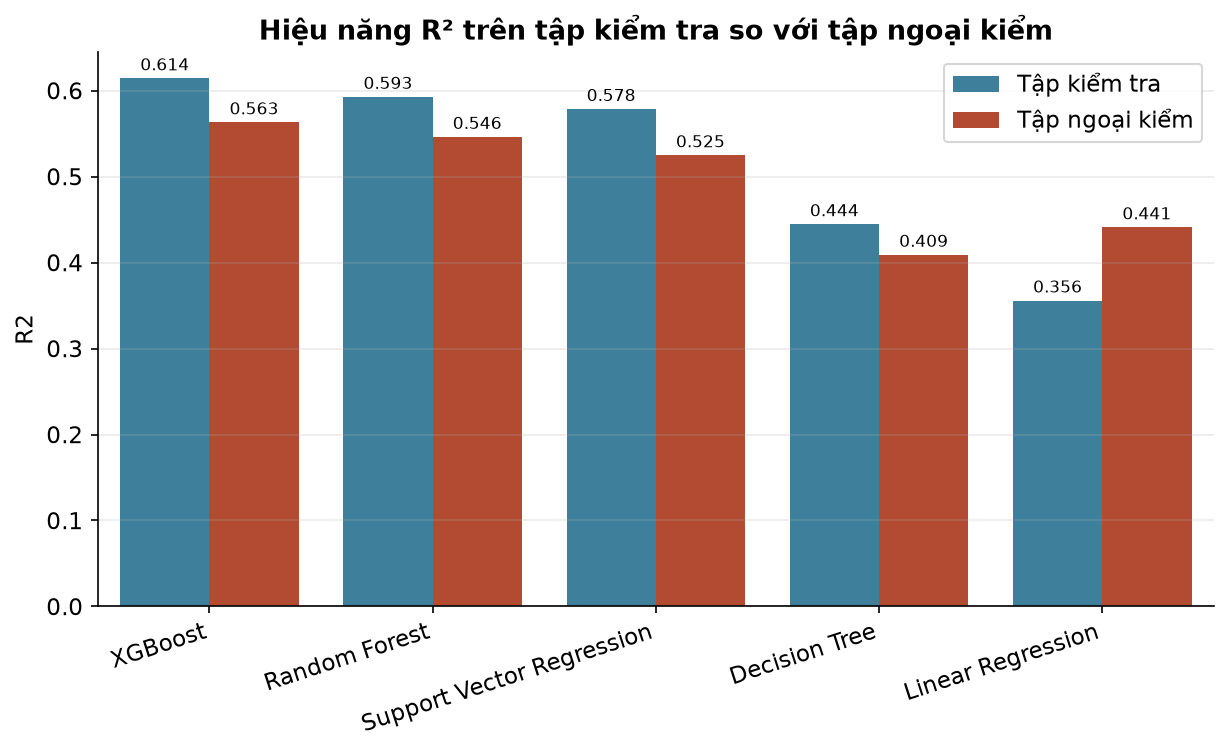
\includegraphics[width=0.92\textwidth]{hou_ood_comparison.png}
\caption[So sánh $R^2$ giữa tập kiểm tra và tập ngoại kiểm]%
{So sánh $R^2$ của năm mô hình giữa tập kiểm tra và tập ngoại kiểm}
\label{fig:hou-ood}
\end{figure}

\begin{table}[H]
\centering
\caption{Kết quả trên tập ngoại kiểm (3.023 tin chưa từng dùng trong phát triển)}
\label{tab:ood-hou}
\small
\begin{tabular}{@{}lrrrr@{}}
\toprule
\textbf{Mô hình} & \textbf{MAE} & \textbf{RMSE} & \textbf{$R^2$} & \textbf{$\Delta R^2$ so với kiểm tra} \\
\midrule
XGBoost                   & \textbf{1{,}1070} & \textbf{1{,}4651} & \textbf{0{,}5629} & $-0{,}0512$ \\
Random Forest             & 1{,}1310 & 1{,}4932 & 0{,}5460 & $-0{,}0465$ \\
Support Vector Regression & 1{,}1302 & 1{,}5279 & 0{,}5246 & $-0{,}0538$ \\
Linear Regression         & 1{,}2935 & 1{,}6571 & 0{,}4408 & $+0{,}0851$ \\
Decision Tree             & 1{,}2736 & 1{,}7038 & 0{,}4088 & $-0{,}0356$ \\
\bottomrule
\end{tabular}
\end{table}

\nhanxet{Khác hẳn bài toán tiểu đường, ở đây kết quả ngoại kiểm \textbf{ổn định
và có thể tin được}: thứ hạng bốn mô hình đầu giữ nguyên hoàn toàn, và mức sụt
$R^2$ đều đặn quanh $0{,}05$ cho ba mô hình dẫn đầu. Sự khác biệt đến từ kích
thước tập: $3.023$ tin so với $77$ ca --- gấp gần 40 lần, nên dao động lấy mẫu
nhỏ hơn nhiều.

Mức sụt $0{,}05$ là biên độ lành mạnh: nó xác nhận điểm số trên tập kiểm tra có
lạc quan chút ít (do đã dùng tập ấy để chọn mô hình) nhưng không phải học thuộc.
Riêng Linear Regression \emph{tăng} $R^2$ --- mô hình có độ chệch cao thì ít
nhạy với việc đổi tập, đúng như lý thuyết dự đoán.}

\section{Mức độ quan trọng của đặc trưng}
\label{sec:importance-hou}

\begin{figure}[H]
\centering
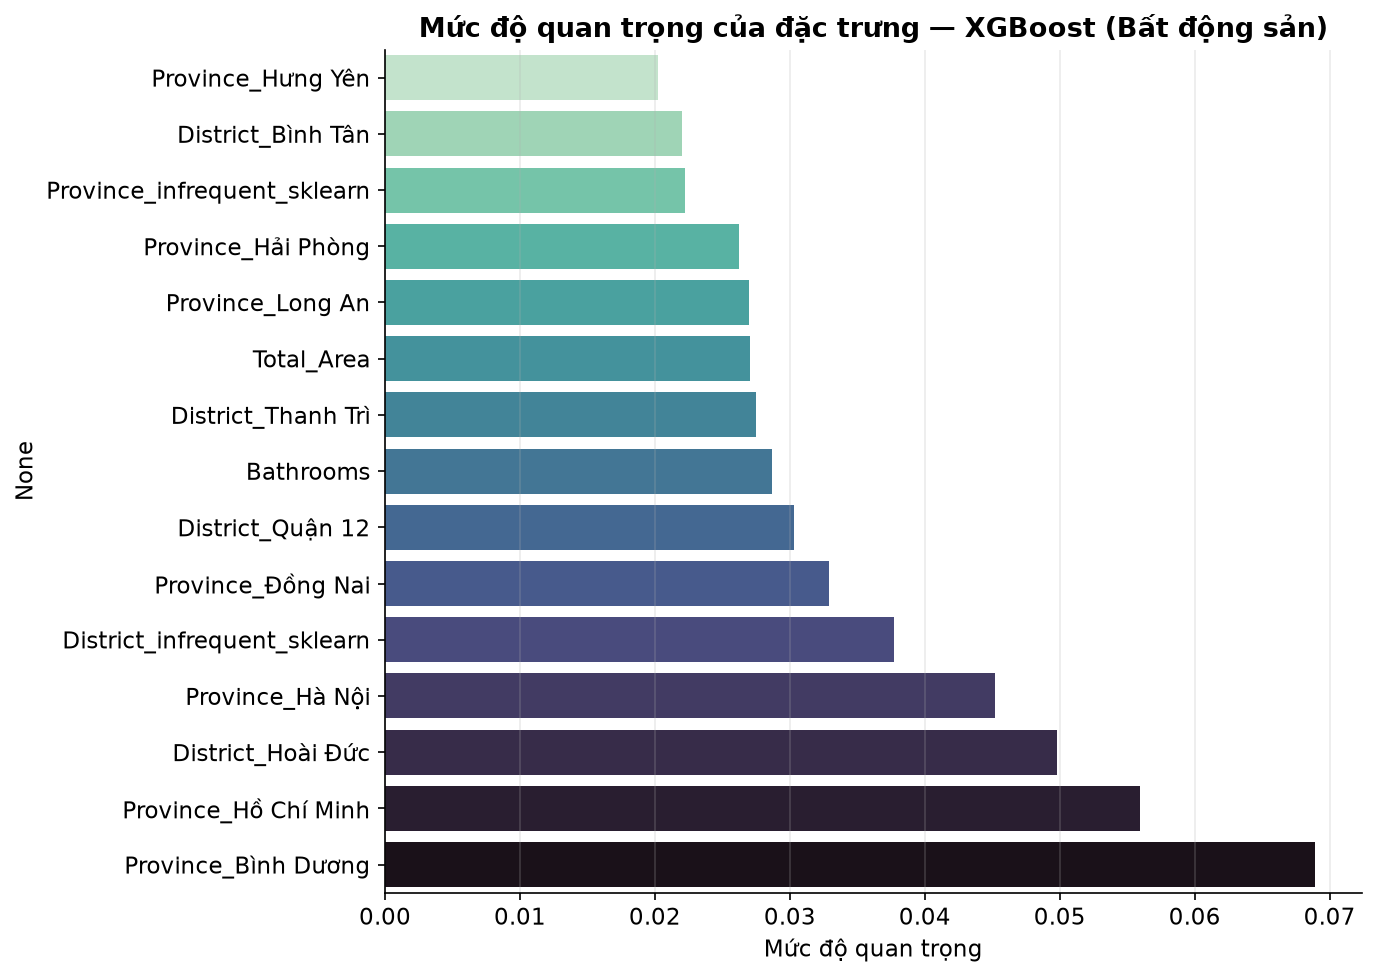
\includegraphics[width=0.9\textwidth]{hou_feature_importance.png}
\caption[Mức độ quan trọng của đặc trưng theo XGBoost]%
{Mức độ quan trọng của 15 đặc trưng dẫn đầu theo mô hình XGBoost}
\label{fig:hou-importance}
\end{figure}

\bieudo{Biểu đồ cột ngang, 15 cột one-hot dẫn đầu.}

\phanphoi{Phân bố phân mảnh --- không cột đơn lẻ nào vượt $0{,}07$, nhưng các cột
dẫn đầu gần như đều thuộc cùng hai nhóm gốc.}

\chitiet{Dẫn đầu là \texttt{Province\_Bình Dương} $0{,}069$, rồi
\texttt{Province\_Hồ Chí Minh} $0{,}056$, \texttt{District\_Hoài Đức} $0{,}050$,
\texttt{Province\_Hà Nội} $0{,}046$. Đặc trưng định lượng đầu tiên xuất hiện là
\texttt{Bathrooms} và \texttt{Total\_Area}, cả hai quanh $0{,}028$.}

\begin{table}[H]
\centering
\caption{Mức quan trọng cộng dồn theo nhóm đặc trưng gốc}
\label{tab:importance-grouped}
\small
\begin{tabular}{@{}lrlr@{}}
\toprule
\textbf{Nhóm đặc trưng} & \textbf{Tổng} & \textbf{Nhóm đặc trưng} & \textbf{Tổng} \\
\midrule
\texttt{District}       & \textbf{0{,}4301} & \texttt{Floors}         & 0{,}0122 \\
\texttt{Province}       & \textbf{0{,}4235} & \texttt{Access Road}    & 0{,}0075 \\
\texttt{Bathrooms}      & 0{,}0287 & \texttt{Area}           & 0{,}0072 \\
\texttt{Total\_Area}    & 0{,}0270 & \texttt{Bedrooms}       & 0{,}0047 \\
\texttt{House direction}& 0{,}0217 & \texttt{Frontage\_Ratio}& 0{,}0041 \\
\texttt{Legal status}   & 0{,}0133 & \texttt{Room\_Density}  & 0{,}0038 \\
\texttt{Furniture state}& 0{,}0131 & \texttt{Frontage}       & 0{,}0031 \\
\bottomrule
\end{tabular}
\end{table}

\begin{phathien}{Hai biến vị trí chiếm 85\% toàn bộ năng lực quyết định}
Cộng dồn theo nhóm gốc cho một con số dứt khoát: \texttt{District} $+$
\texttt{Province} $= 0{,}8536$, tức \textbf{85,4\%} tổng mức quan trọng. Mười
hai nhóm đặc trưng còn lại --- gồm toàn bộ thuộc tính vật lý và pháp lý --- chia
nhau $14{,}6\%$ còn lại.

Con số này giải thích trọn vẹn kết quả Thực nghiệm~3: bỏ biến định danh đi thì
mất đúng phần lớn nhất của cấu trúc, và $R^2$ tụt từ $0{,}5903$ xuống $0{,}3340$.

Nó cũng khép lại nghịch lý ở Hình~\ref{fig:hou-bar-legal}: \texttt{Legal status}
có trung bình biên gần như phẳng nhưng vẫn nhận mức quan trọng $0{,}0133$ --- gấp
gần bốn lần \texttt{Frontage}. Mô hình cây khai thác được quan hệ \emph{có điều
kiện} mà trung bình biên không nhìn thấy.

Câu ngạn ngữ ``vị trí, vị trí, vị trí'' của giới bất động sản, ở tập dữ liệu
này, có một con số cụ thể: $85{,}4\%$.
\end{phathien}

\section{Tích hợp Đồ thị Tri thức Đô thị -- Tài chính}
\label{sec:kg-hou}

\subsection{Phân khúc thị trường}

\begin{table}[H]
\centering
\caption{Ba phân khúc thị trường và gói tín dụng tương ứng}
\label{tab:phankhuc-hou}
\small
\begin{tabularx}{\textwidth}{@{}L{3.2cm}L{1.5cm}L{3.4cm}rrX@{}}
\toprule
\textbf{Phân khúc} & \textbf{Ngưỡng} & \textbf{Gói vay} & \textbf{LTV} & \textbf{Lãi suất} & \textbf{Kỳ hạn} \\
\midrule
Cao cấp    & $\ge 8{,}0$ tỷ & Bất động sản Cao cấp & 70\% & 8{,}5\% & 25 năm \\
Trung cấp  & $\ge 4{,}5$ tỷ & Mua nhà Linh hoạt    & 75\% & 7{,}9\% & 20 năm \\
Bình dân   & $\ge 0{,}0$ tỷ & Nhà ở Xã hội         & 80\% & 4{,}8\% & 25 năm \\
\bottomrule
\end{tabularx}
\end{table}

\subsection{Đồ thị của một ca cụ thể}

\begin{figure}[H]
\centering
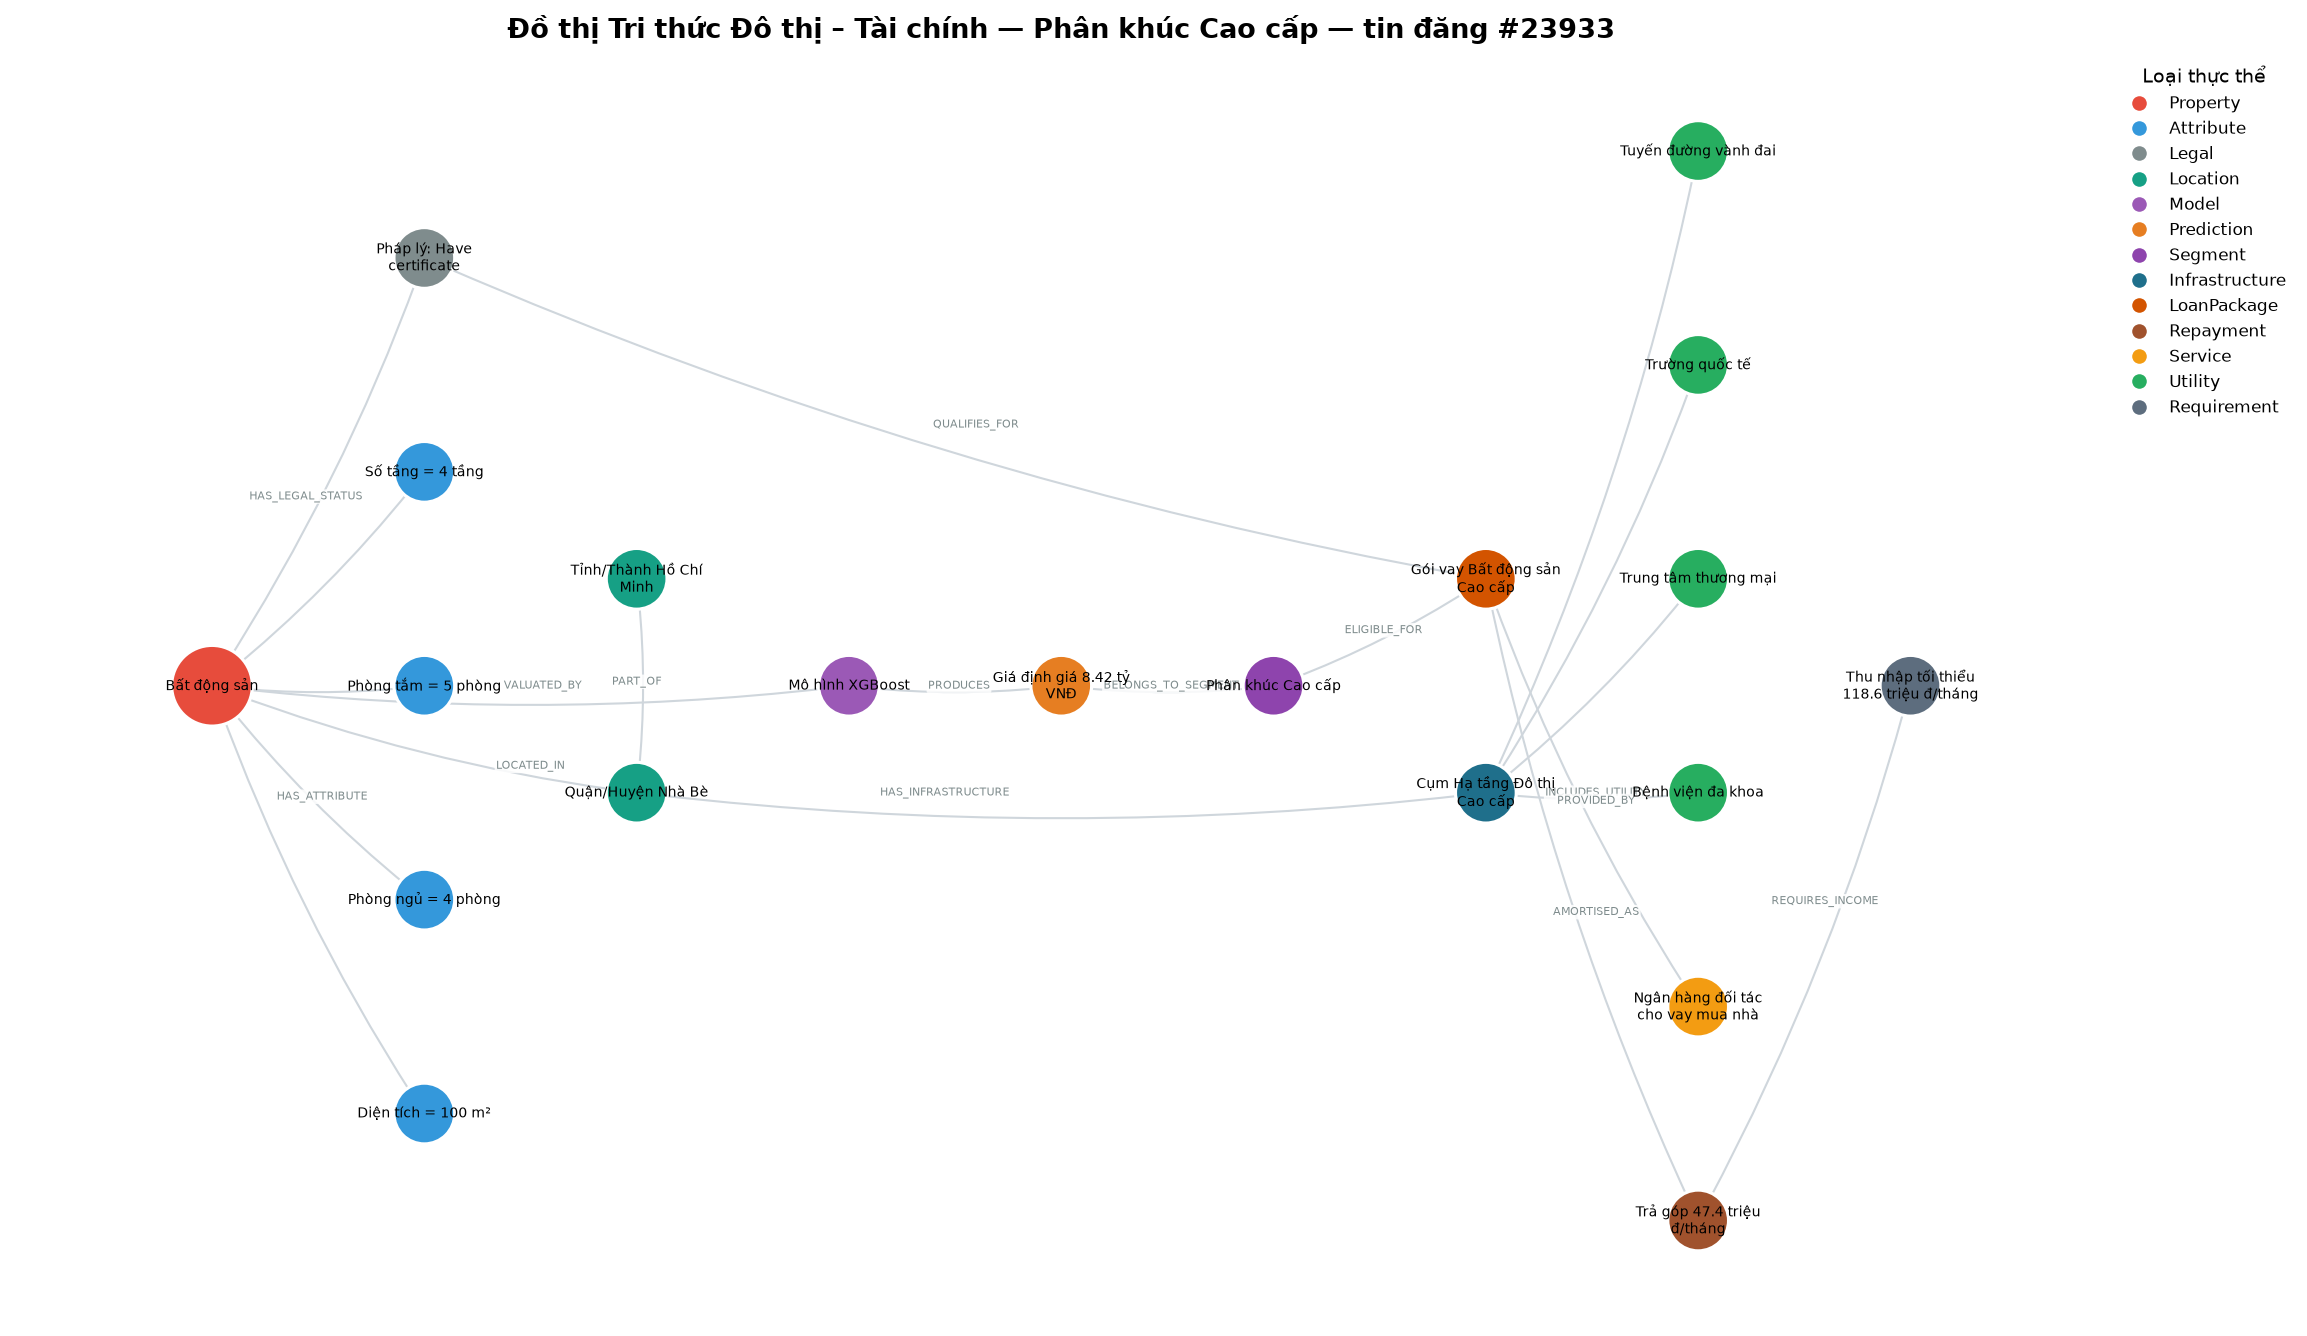
\includegraphics[width=\textwidth]{kg_property.png}
\caption[Đồ thị Tri thức Đô thị -- Tài chính của tin đăng \#23933]%
{Đồ thị Tri thức Đô thị -- Tài chính của tin đăng \#23933 --- Phân khúc Cao cấp,
20 thực thể và 20 cạnh}
\label{fig:kg-property}
\end{figure}

\bieudo{Đồ thị có hướng vẽ theo bố cục phân tầng, màu nút mã hoá loại thực thể.}

\phanphoi{Cấu trúc hình thoi: mở rộng ở tầng thuộc tính, thắt lại tại nút định
giá và nút phân khúc, rồi mở rộng lần nữa ở tầng tài chính và hạ tầng.}

\chitiet{Bên trái là bốn thuộc tính vật lý cùng nút pháp lý. Ở giữa là chuỗi
Bất động sản $\to$ Quận Nhà Bè $\to$ Tỉnh Hồ Chí Minh và song song là Mô hình
XGBoost $\to$ Giá $8{,}42$ tỷ $\to$ Phân khúc Cao cấp. Bên phải chia hai nhánh:
nhánh tài chính đi qua Gói vay $\to$ Trả góp $47{,}5$ triệu/tháng $\to$ Thu nhập
tối thiểu $118{,}7$ triệu/tháng, và nhánh hạ tầng đi qua Cụm Hạ tầng Đô thị Cao
cấp tới bốn tiện ích.}

\subsection{Gói tài chính mua nhà}
\label{sec:goi-tai-chinh}

Áp dụng công thức niên kim~\eqref{eq:nienkim} và ngưỡng DTI~\eqref{eq:dti} cho
tin đăng \#23933:

\begin{table}[H]
\centering
\caption{Hồ sơ tài chính đầy đủ cho tin đăng \#23933 (giá dự báo 8,42 tỷ VNĐ)}
\label{tab:taichinh-hou}
\small
\begin{tabularx}{\textwidth}{@{}L{5.2cm}R{3.4cm}X@{}}
\toprule
\textbf{Khoản mục} & \textbf{Giá trị} & \textbf{Cách tính} \\
\midrule
Giá định giá            & 8{,}42 tỷ đ    & Mô hình XGBoost \\
Tỷ lệ cho vay (LTV)     & 70\%           & Theo phân khúc Cao cấp \\
Hạn mức vay $P$         & \textbf{5{,}89 tỷ đ} & $8{,}42\times0{,}70$ \\
Vốn tự có tối thiểu     & 2{,}53 tỷ đ    & $8{,}42-5{,}89$ \\
Lãi suất danh nghĩa     & 8{,}5\%/năm    & Mặt bằng công bố \\
Kỳ hạn                  & 25 năm (300 kỳ) & \\
\textbf{Trả góp hằng tháng $M$} & \textbf{47{,}5 triệu đ} & Công thức~\eqref{eq:nienkim} \\
Tổng tiền lãi           & 8{,}34 tỷ đ    & $Mn - P$ \\
\textbf{Thu nhập tối thiểu} & \textbf{118{,}7 triệu đ/tháng} & $M/0{,}40$, công thức~\eqref{eq:dti} \\
\bottomrule
\end{tabularx}
\end{table}

\begin{phathien}{Tổng tiền lãi vượt cả dư nợ gốc}
Với kỳ hạn 25 năm ở lãi suất $8{,}5\%$/năm, tổng tiền lãi là $8{,}34$ tỷ trên
khoản vay gốc $5{,}89$ tỷ --- tức \textbf{142\% dư nợ gốc}. Người vay trả về cho
ngân hàng tổng cộng $14{,}23$ tỷ để mua một căn nhà định giá $8{,}42$ tỷ.

Đây là con số mà bảng quảng cáo gói vay hiếm khi đặt cạnh con số trả góp hằng
tháng, và hệ thống hiển thị nó tường minh. Lịch trả nợ còn cho thấy một điều
nữa: năm đầu tiên trả $498$ triệu tiền lãi nhưng chỉ giảm được $71$ triệu dư
nợ --- phần lãi dồn hết về đầu kỳ, nên trả trước hạn trong vài năm đầu là lúc
tiết kiệm được nhiều nhất.

Con số \textbf{thu nhập tối thiểu $118{,}7$ triệu đồng mỗi tháng} là câu trả lời
thẳng thắn nhất mà hệ thống đưa ra: nó nói cho người dùng biết căn nhà này có
nằm trong tầm với của họ hay không, điều mà con số ``$8{,}42$ tỷ'' đơn thuần
không nói được.
\end{phathien}

\subsection{Tiện ích hạ tầng đô thị}

\begin{table}[H]
\centering
\caption{Cụm hạ tầng tiện ích theo phân khúc, phân loại theo bốn nhóm chức năng}
\label{tab:tienich-hou}
\small
\begin{tabularx}{\textwidth}{@{}L{3.4cm}rXX@{}}
\toprule
\textbf{Cụm} & \textbf{Bán kính} & \textbf{Tiện ích} & \textbf{Nhóm chức năng} \\
\midrule
\multirow{4}{*}{Cao cấp}   & \multirow{4}{*}{2{,}0 km} & Trung tâm thương mại & Thương mại \\
 & & Trường quốc tế        & Giáo dục \\
 & & Bệnh viện đa khoa     & Y tế \\
 & & Tuyến đường vành đai  & Giao thông \\
\midrule
\multirow{4}{*}{Trung cấp} & \multirow{4}{*}{1{,}5 km} & Siêu thị & Thương mại \\
 & & Trường công lập       & Giáo dục \\
 & & Trạm y tế phường      & Y tế \\
 & & Tuyến xe buýt nội đô  & Giao thông \\
\midrule
\multirow{4}{*}{Cơ bản}    & \multirow{4}{*}{3{,}0 km} & Chợ dân sinh & Thương mại \\
 & & Trường tiểu học       & Giáo dục \\
 & & Phòng khám đa khoa    & Y tế \\
 & & Tuyến xe buýt liên huyện & Giao thông \\
\bottomrule
\end{tabularx}
\end{table}

\nhanxet{Bốn nhóm chức năng được giữ cố định qua cả ba phân khúc, chỉ đổi mức
độ. Cách tổ chức này cho phép so sánh trực tiếp: cùng nhu cầu y tế, phân khúc
cao cấp có bệnh viện đa khoa trong bán kính $2$ km còn phân khúc cơ bản có phòng
khám khu vực trong bán kính $3$ km.

Xin nhắc lại ranh giới ở Mục~\ref{sec:ranh-gioi-so-lieu}: đây là mô hình hoá
theo phân khúc, \textbf{không phải} khảo sát thực địa từng quận --- tập dữ liệu
gốc chỉ có địa chỉ hành chính, không có toạ độ, nên không thể suy ra khoảng cách
thật tới một siêu thị cụ thể.}

\section{Ứng dụng web}
\label{sec:app-hou}

\begin{figure}[H]
\centering
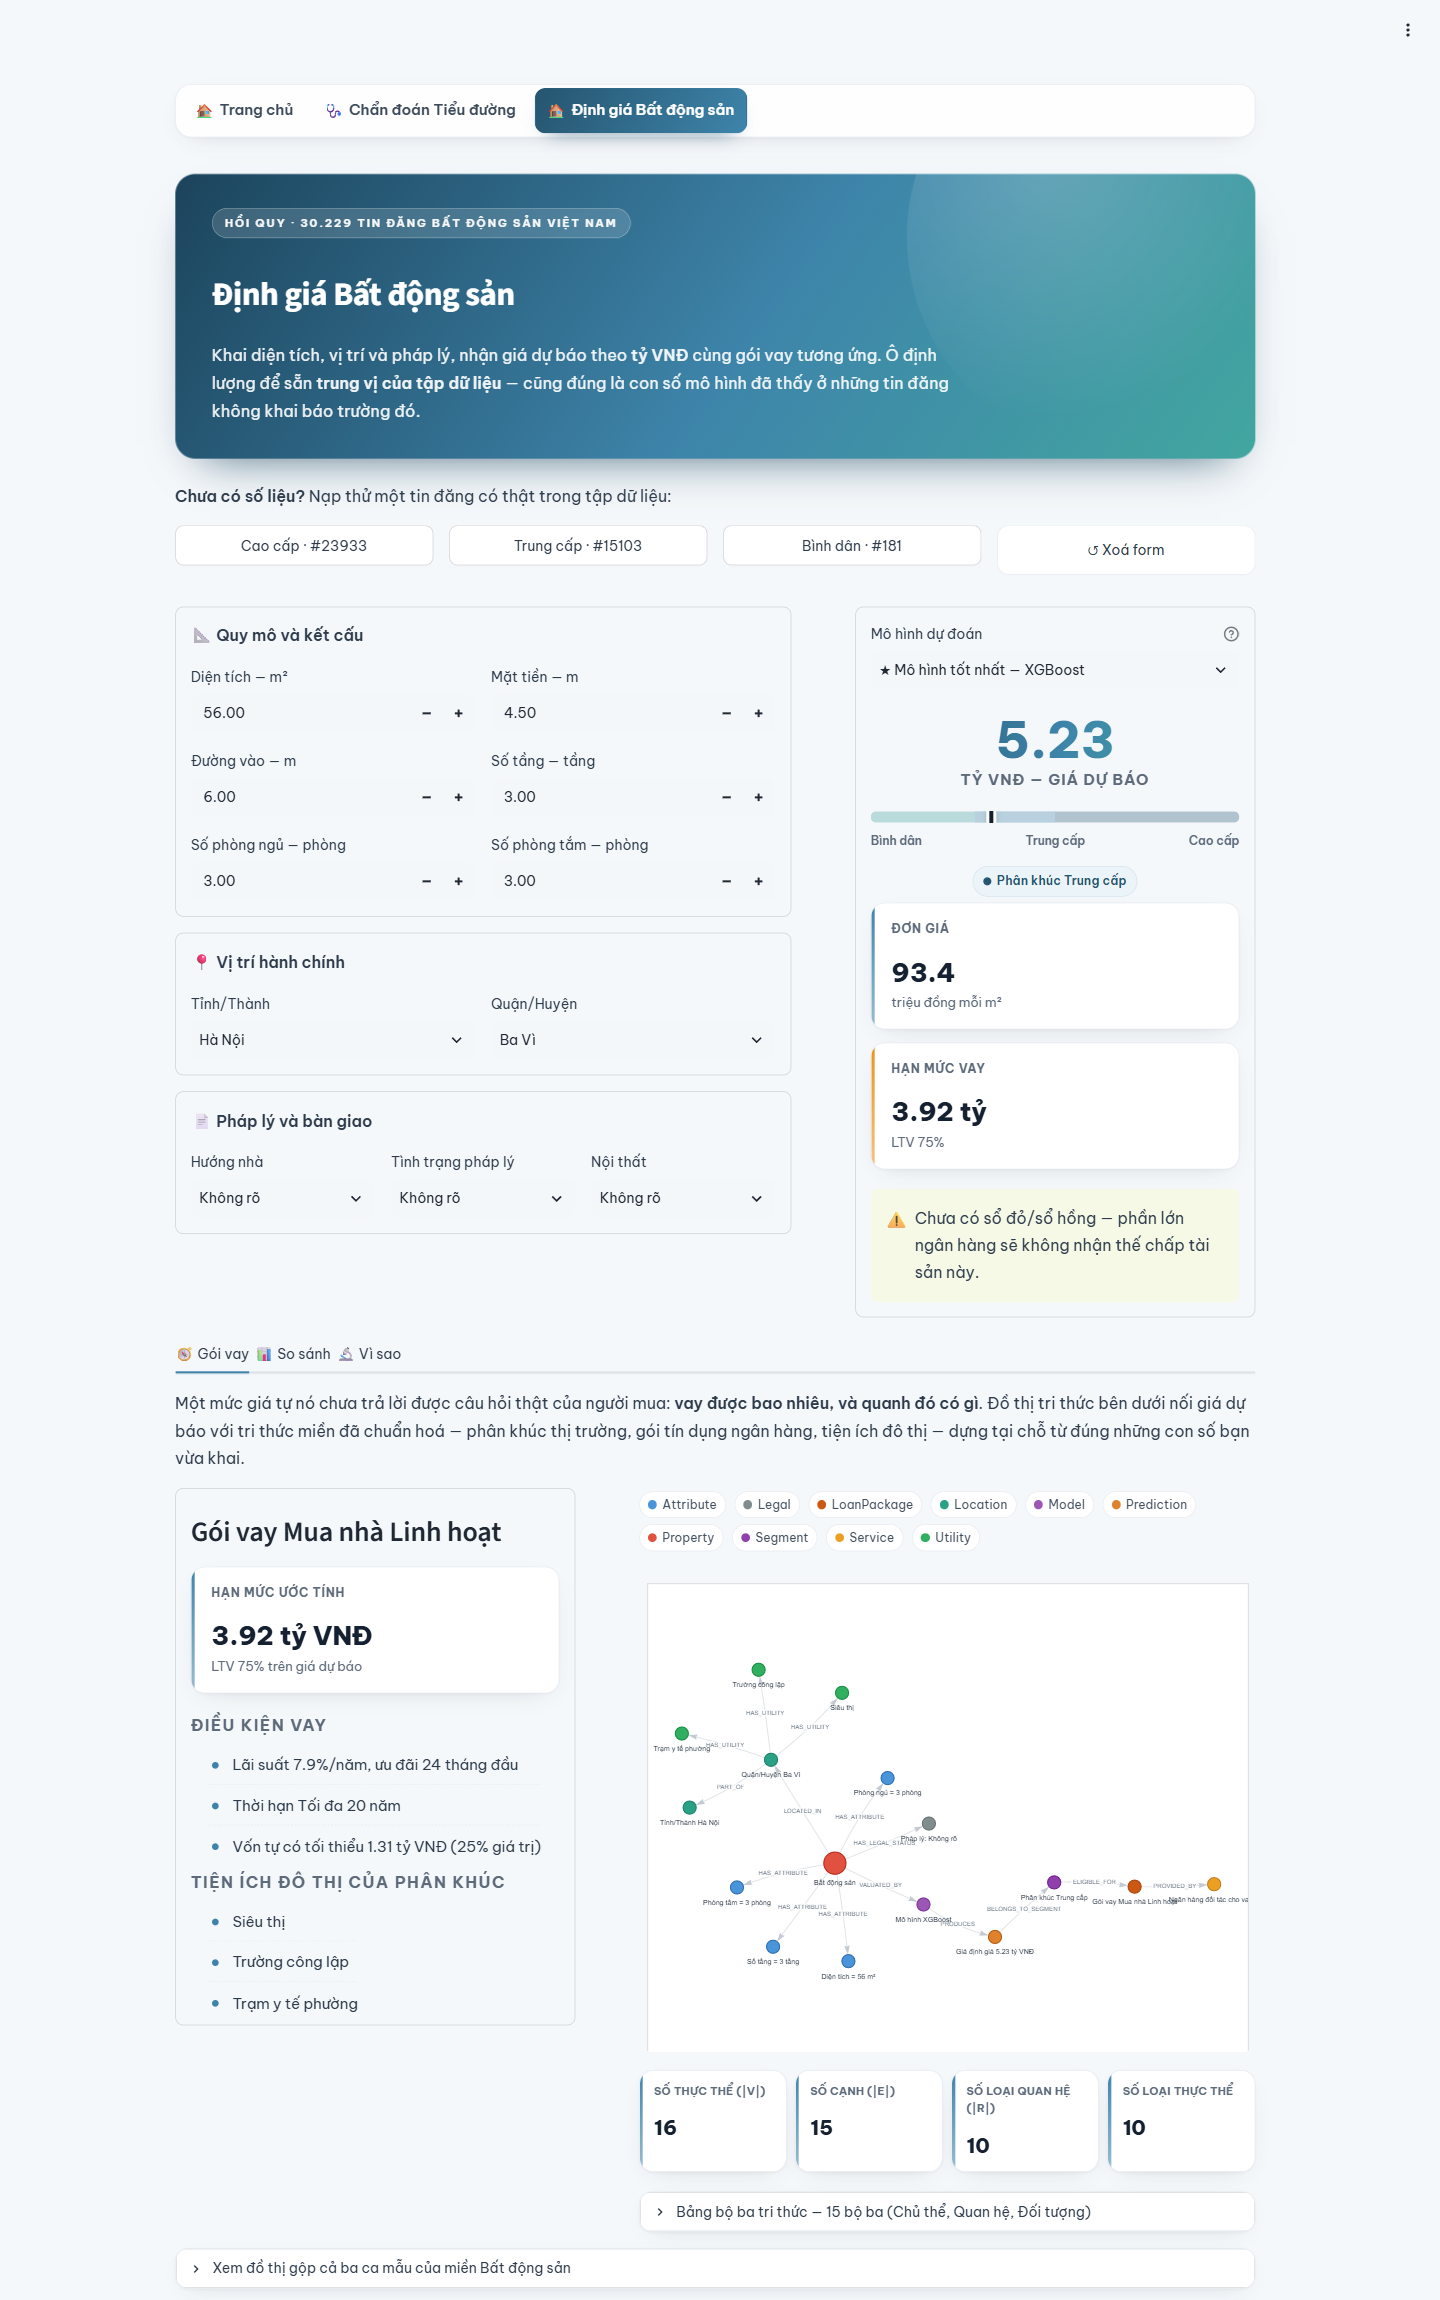
\includegraphics[width=0.86\textwidth]{app-desktop-3-dinh-gia.png}
\caption[Giao diện trang Định giá Bất động sản trên máy tính]%
{Giao diện trang Định giá Bất động sản trên máy tính --- biểu mẫu khai thuộc
tính, giá dự báo, hạn mức vay và đồ thị tri thức}
\label{fig:app-hou-desktop}
\end{figure}

\bieudo{Ảnh chụp màn hình bản đã triển khai công khai, khổ máy tính $1440$ px.}

\chitiet{Cột trái là biểu mẫu chia ba khối --- quy mô và kết cấu, vị trí hành
chính, pháp lý và bàn giao --- trong đó danh sách Quận/Huyện được lọc động theo
Tỉnh/Thành đã chọn. Cột phải hiển thị giá dự báo cỡ lớn, thanh phân khúc, đơn
giá mỗi m$^2$ và hạn mức vay. Bốn tab phía dưới: Gói vay, Hạ tầng \& Tài chính,
So sánh, Vì sao.}

\nhanxet{Tab ``Hạ tầng \& Tài chính'' là nơi hệ thống trả lời trọn vẹn câu hỏi
của người mua: bốn thẻ số ở đầu tab cho trả góp hằng tháng, thu nhập tối thiểu,
vốn tự có và tổng tiền lãi; bảng bên trái liệt kê điều khoản vay; bảng bên phải
là lịch trả nợ theo từng năm với cột trả gốc, trả lãi và dư nợ còn lại.

Ứng dụng cũng hiển thị cảnh báo khi tin đăng thiếu giấy tờ: ``chưa có sổ đỏ hoặc
sổ hồng --- phần lớn ngân hàng sẽ không nhận thế chấp tài sản này'', lấy trực
tiếp từ quan hệ \texttt{QUALIFIES\_FOR} trong đồ thị tri thức.}

\begin{figure}[H]
\centering
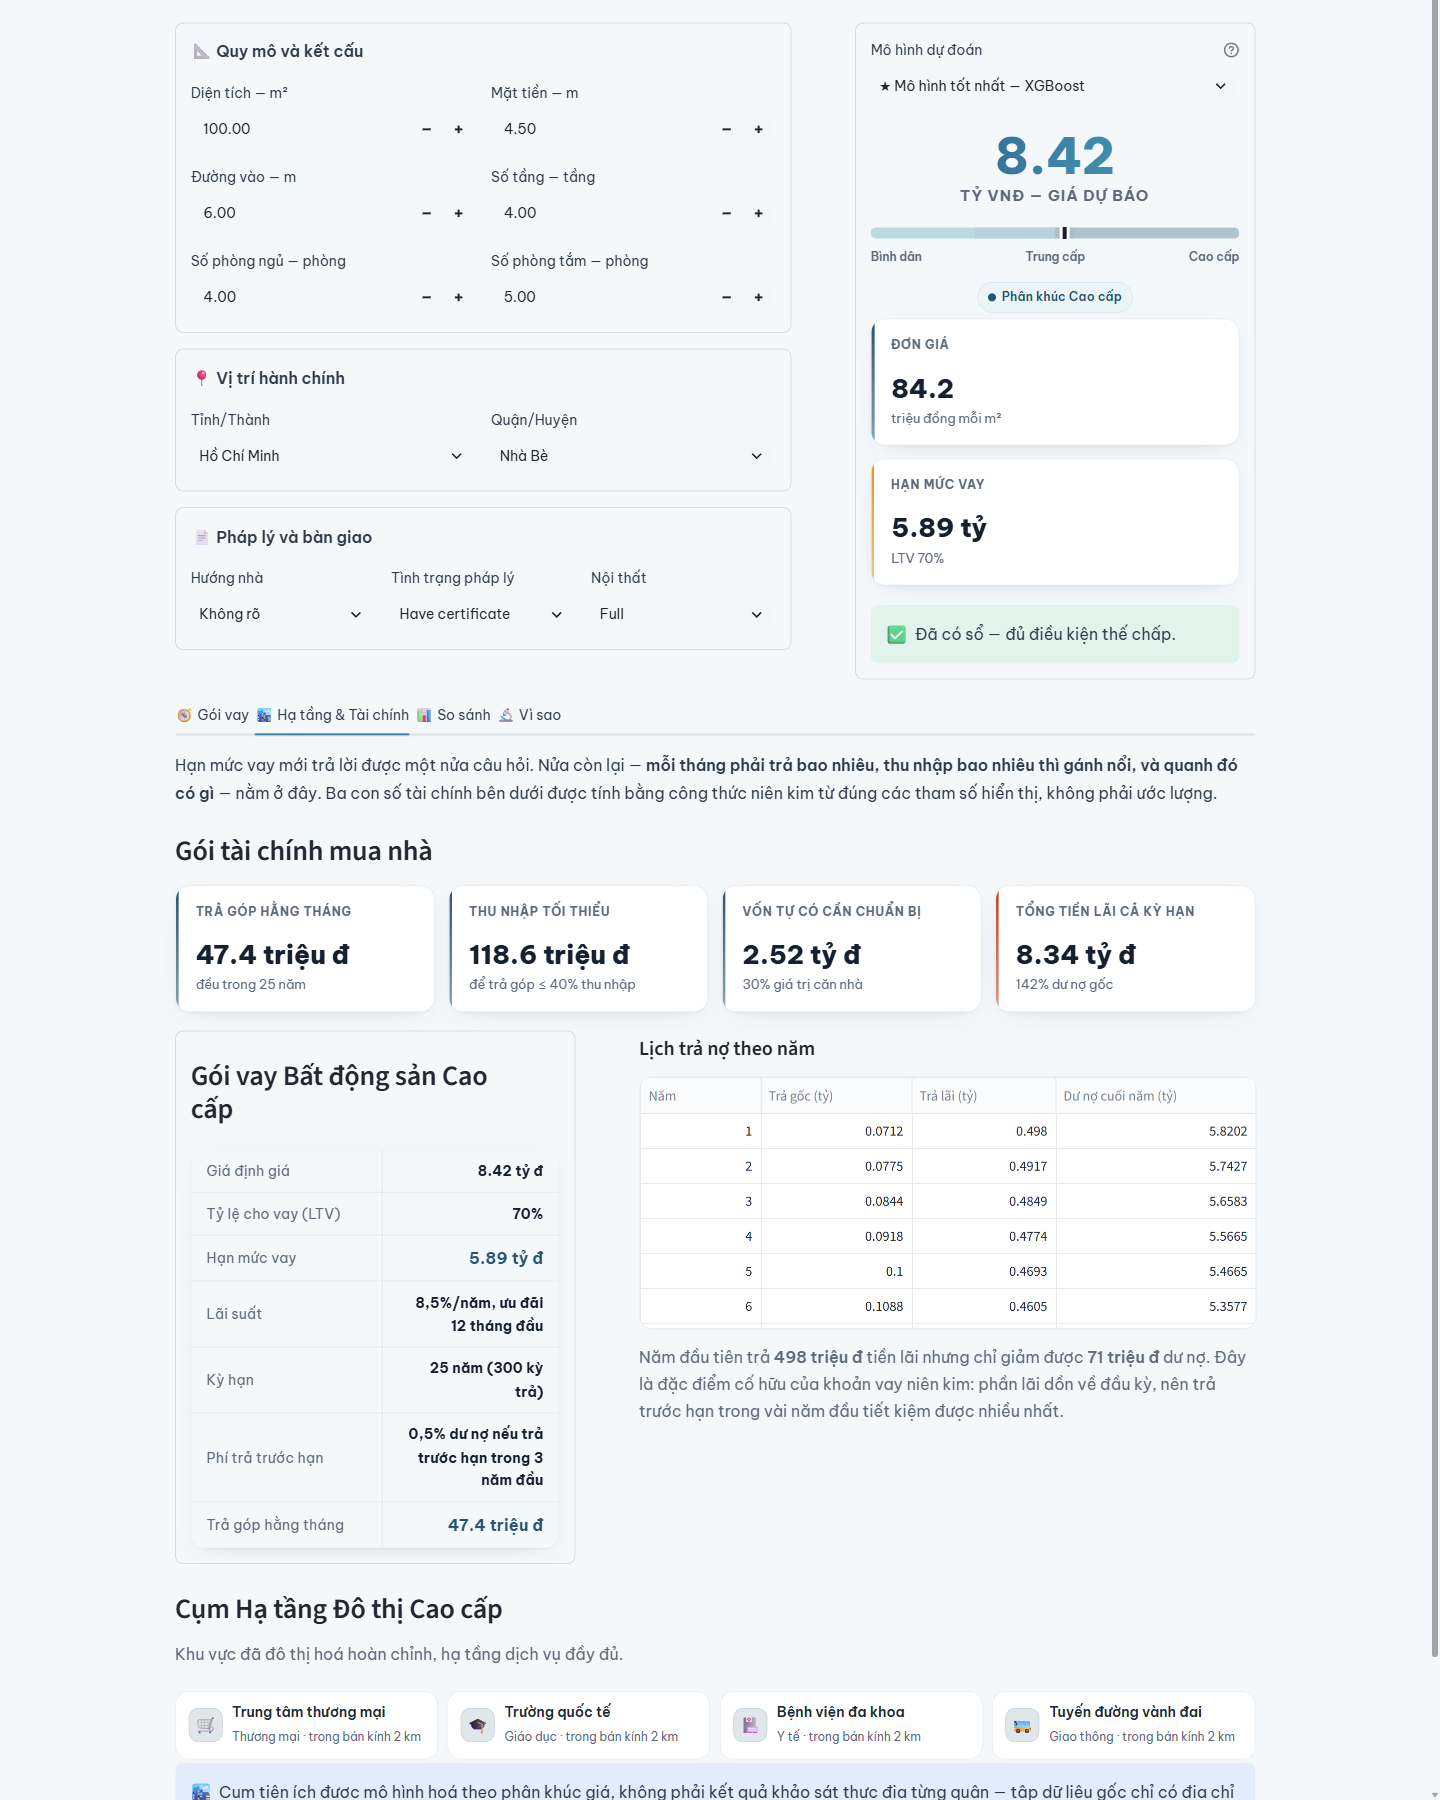
\includegraphics[width=0.86\textwidth]{app-desktop-5-ha-tang-tai-chinh.png}
\caption[Tab Hạ tầng \& Tài chính --- trả góp, lịch trả nợ và cụm tiện ích]%
{Tab \emph{Hạ tầng \& Tài chính} --- bốn chỉ số tài chính, bảng điều khoản vay,
lịch trả nợ theo năm và cụm tiện ích hạ tầng}
\label{fig:app-hou-tai-chinh}
\end{figure}

\bieudo{Ảnh chụp màn hình tab thứ hai của trang Định giá.}

\chitiet{Bốn thẻ số ở đầu tab: trả góp $47{,}4$ triệu đồng mỗi tháng, thu nhập
tối thiểu $118{,}6$ triệu đồng, vốn tự có $2{,}52$ tỷ và tổng tiền lãi
$8{,}34$ tỷ --- bằng $142\%$ dư nợ gốc. Bảng bên trái liệt kê bảy dòng điều
khoản vay; bảng bên phải là lịch trả nợ theo năm với ba cột trả gốc, trả lãi và
dư nợ cuối năm. Cuối tab là bốn thẻ tiện ích, mỗi thẻ ghi nhóm chức năng và bán
kính tiếp cận.}

\nhanxet{Con số trên giao diện chênh nhẹ so với Bảng~\ref{tab:taichinh-hou}
($47{,}4$ so với $47{,}5$ triệu đồng) vì ứng dụng tính trên giá dự báo đầy đủ
của mô hình, còn bảng trong báo cáo tính trên con số $8{,}42$ tỷ đã làm tròn để
hiển thị. Đây là chênh lệch làm tròn, không phải hai phép tính khác nhau.

Dòng chú thích dưới lịch trả nợ là chỗ hệ thống nói ra điều mà bảng quảng cáo
gói vay thường không nói: năm đầu tiên trả $498$ triệu tiền lãi nhưng chỉ giảm
được $71$ triệu dư nợ.}

\begin{figure}[H]
\centering
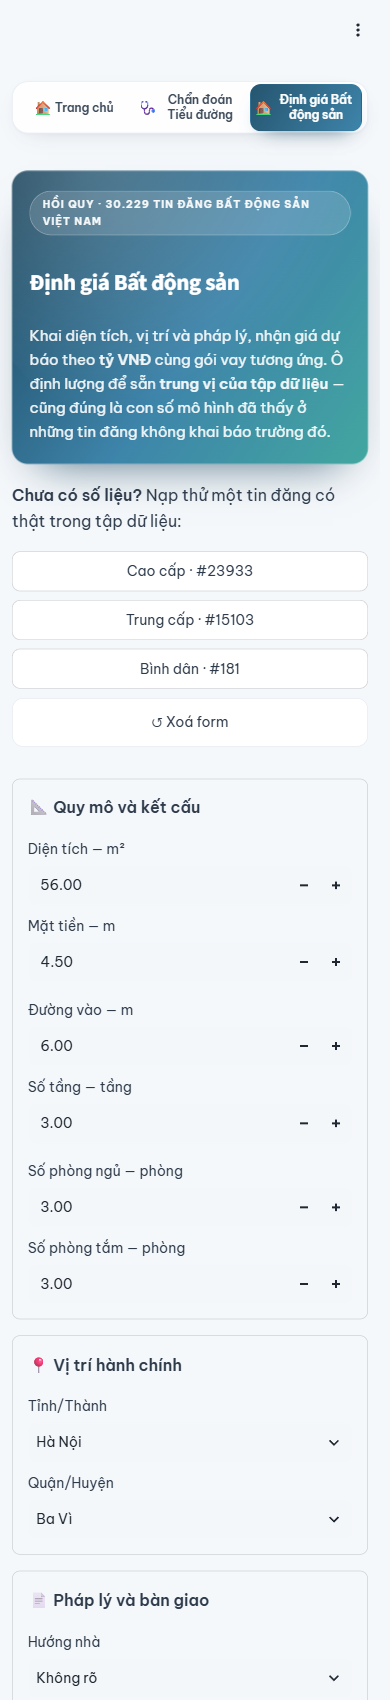
\includegraphics[width=0.34\textwidth]{app-mobile-3-dinh-gia.png}
\caption[Giao diện trang Định giá trên điện thoại]%
{Giao diện trang Định giá trên điện thoại, khổ $390$ px}
\label{fig:app-hou-mobile}
\end{figure}

% =====================================================================
%  Chương 4 — Kết luận và Hướng phát triển
% =====================================================================
\chapter{Kết luận và Hướng phát triển}
\label{ch:ketluan}

\section{Tổng kết kết quả}
\label{sec:tongket}

Hai hệ thống thông minh đã được xây dựng trọn vẹn, mỗi hệ thống đi hết chuỗi
sáu tầng ở Hình~\ref{fig:sodo-hethong}: từ dữ liệu thật, qua biểu diễn véc-tơ,
qua năm mô hình học máy được so sánh dưới cùng một giao thức, tới dự đoán, và
cuối cùng tới một khuyến nghị hành động \emph{có chi phí xác định}.

\begin{table}[H]
\centering
\caption{Tổng kết hai hệ thống}
\label{tab:tongket}
\small
\begin{tabularx}{\textwidth}{@{}L{3.4cm}XX@{}}
\toprule
 & \textbf{Hệ thống 1 --- Tiểu đường} & \textbf{Hệ thống 2 --- Bất động sản} \\
\midrule
Loại bài toán   & Phân lớp nhị phân & Hồi quy \\
Quy mô dữ liệu  & 768 hồ sơ & 30.229 tin đăng \\
Số chiều biểu diễn & 12 & 84 \\
Mô hình cơ sở   & Accuracy $0{,}6547$, Recall $0{,}0000$ & MAE $1{,}8587$, $R^2 = -0{,}0008$ \\
Mô hình tốt nhất & K-Nearest Neighbors, $F_1 = 0{,}6809$ & XGBoost, $R^2 = 0{,}6141$ \\
Độ đo phụ tốt nhất & ROC-AUC $0{,}8709$ (Logistic Regression) & MAE $1{,}0493$ tỷ VNĐ \\
Cải thiện so với cơ sở & $F_1$: $0 \to 0{,}68$ & MAE giảm $43{,}5\%$ \\
Thuật toán hay biểu diễn chi phối & \textbf{Thuật toán}, gấp 6 lần & \textbf{Ngang bằng} \\
Đồ thị tri thức & 5 tầng, gói chăm sóc có chi phí & 5 tầng, gói vay có lịch trả nợ \\
\bottomrule
\end{tabularx}
\end{table}

Về hạ tầng: một lệnh \texttt{python run\_pipeline.py} tái tạo toàn bộ trong
khoảng 90 giây; 355 bài kiểm thử tự động chạy trong 17 giây; Đồ thị Tri thức
gồm 117 thực thể, 133 cạnh và 28 loại quan hệ đã nạp thật lên máy chủ Neo4j
Aura~\cite{neo4j}; ứng dụng web~\cite{streamlit} đã triển khai công khai và truy cập được từ internet~\cite{repo}.

\section{Phân tích khoa học --- bảy phát hiện}
\label{sec:phantich}

Mục này đáp ứng yêu cầu R10. Điểm chung của bảy phát hiện dưới đây: chúng đều
\emph{bác bỏ} một giả định mà người viết tin là đúng lúc mới bắt đầu, và mỗi
phát hiện đều kèm bằng chứng định lượng tái lập được.

\subsection{Phát hiện 1 --- Kết quả vượt trần tài liệu là dấu hiệu của lỗi}

Bản triển khai đầu tiên điền khuyết bằng trung vị theo nhóm \texttt{Outcome} và
đạt Accuracy $0{,}8705$ --- vượt hẳn trần $0{,}77$--$0{,}79$ mà mọi nghiên cứu
công bố trên tập Pima đều dừng lại. Nguyên nhân là rò rỉ nhãn: với
\texttt{Insulin} khuyết $374/768$ và \texttt{SkinThickness} khuyết $227/768$,
gần một nửa dữ liệu sau khi điền đã mang dấu vết của chính nhãn cần dự đoán.
Đưa \texttt{SimpleImputer} vào trong \texttt{Pipeline} đưa con số về $0{,}7914$.

\textbf{Bài học phương pháp:} đối chiếu kết quả với trần đã công bố trong tài
liệu là một bước kiểm tra rẻ tiền và hiệu quả bất ngờ. Một con số đẹp hơn dự
kiến đáng để đi tìm lỗi, không phải để ăn mừng.

\subsection{Phát hiện 2 --- Quét ngưỡng đòi hỏi mô hình cho xác suất liên tục}

Thực nghiệm quét ngưỡng chạy lần đầu trên Decision Tree sâu 6 tầng cho bảy
ngưỡng từ $0{,}50$ xuống $0{,}20$ ra \emph{đúng một} kết quả. Cây nông chỉ trả
về vài giá trị xác suất rời rạc nên phần lớn ngưỡng rơi vào cùng một khoảng.
Hiện tượng này để lại một dấu vết nhìn thấy được: đường ROC của Decision Tree ở
Hình~\ref{fig:dia-roc} có dạng gãy khúc thành vài đoạn thẳng dài thay vì cong
mượt như bốn mô hình còn lại. Chuyển sang XGBoost cho 12 mức kết quả khác nhau
trên 13 ngưỡng.

\textbf{Bài học:} một thực nghiệm không cho kết quả có thể là do thực nghiệm sai
thiết kế, không phải do hiệu ứng không tồn tại.

\subsection{Phát hiện 3 --- Cực trị chạm biên dải khảo sát thì chưa phải cực trị}

Bẫy này xuất hiện \textbf{hai lần độc lập}: độ sâu rừng ngẫu nhiên đạt đỉnh ở
$24$ khi dải quét dừng ở $24$, và ngưỡng quyết định đạt đỉnh ở $0{,}20$ khi dải
quét dừng ở $0{,}20$. Cả hai lần đều phải nới dải mới xác nhận được đỉnh thật
(lần lượt là $24$ và $0{,}15$).

\textbf{Bài học:} trước khi kết luận một siêu tham số là tối ưu, hãy kiểm tra nó
không nằm ở đầu mút dải khảo sát. Kiểm tra này rẻ và tự động hoá được --- hàm vẽ
biểu đồ quét ngưỡng trong dự án đã được sửa để tự in cảnh báo ``chạm biên dải
quét'' khi điều đó xảy ra.

\subsection{Phát hiện 4 --- ``Biểu diễn quan trọng hơn thuật toán'' là SAI nếu phát biểu trần}
\label{sec:phanchieu}

Đây là phát hiện trung tâm của cả báo cáo, và nó đáp ứng trực tiếp yêu cầu R13.

Cùng một thiết kế Thực nghiệm~3 --- giữ nguyên thuật toán, chỉ đổi biểu diễn ---
chạy trên hai bài toán cho hai kết luận trái ngược:

\begin{table}[H]
\centering
\caption{Biên độ do biểu diễn so với biên độ do thuật toán, hai bài toán}
\label{tab:biendo-ca-hai}
\small
\begin{tabularx}{\textwidth}{@{}L{5.4cm}R{3.0cm}R{3.2cm}@{}}
\toprule
 & \textbf{Tiểu đường ($F_1$)} & \textbf{Bất động sản ($R^2$)} \\
\midrule
Biên độ do đổi \textbf{biểu diễn}  & 0{,}0300 & 0{,}2563 \\
Biên độ do đổi \textbf{thuật toán} & 0{,}1809 & 0{,}2584 \\
\midrule
Bên nào chi phối & \textbf{Thuật toán} (gấp 6) & \textbf{Ngang bằng} \\
\bottomrule
\end{tabularx}
\end{table}

\textbf{Điều phân biệt hai trường hợp không nằm ở thuật toán, mà nằm ở chỗ phép
biểu diễn có làm thay đổi \emph{lượng} thông tin hay chỉ đổi \emph{dạng} thông
tin đã có.}

\begin{itemize}
  \item Ở bài toán bất động sản, phương án ``chỉ đặc trưng định lượng''
        \textbf{bỏ đi} toàn bộ nhóm biến định danh --- và \texttt{Province} cùng
        \texttt{District} không suy ra được từ bất kỳ cột nào khác. Đây là
        \emph{thêm hoặc bớt thông tin}, nên tác động lớn: $R^2$ mất $0{,}2563$.
  \item Ở bài toán tiểu đường, cả bốn phương án đều dùng đúng tám cột gốc ấy;
        chúng chỉ khác nhau ở chỗ có chuẩn hoá hay không, có nhân hai cột với
        nhau hay không. Đây là \emph{đổi dạng} thông tin đã có, nên tác động nhỏ
        và nằm trọn trong nhiễu lấy mẫu: bốn phương án chỉ phân loại khác nhau
        \textbf{1--9 ca trên 139}.
\end{itemize}

\begin{phathien}{Phát biểu đã được sửa lại cho đúng}
Phát biểu ban đầu --- ``biểu diễn dữ liệu quan trọng hơn thuật toán'' --- không
đứng vững qua kiểm chứng. Phát biểu đúng là:

\begin{quote}
\itshape
Biểu diễn dữ liệu chi phối kết quả khi và chỉ khi nó \textbf{thay đổi lượng
thông tin} có trong biểu diễn. Khi nó chỉ đổi \textbf{dạng} của thông tin đã có
--- chuẩn hoá, rời rạc hoá, nhân hai cột --- thì tác động của nó thường nhỏ hơn
tác động của việc đổi thuật toán, và có thể nằm trọn trong nhiễu lấy mẫu.
\end{quote}

Đây là lý do phải chạy \emph{cùng một thực nghiệm trên hai miền dữ liệu}: một
miền đơn lẻ sẽ cho một kết luận nghe rất thuyết phục và không có cách nào phát
hiện ra nó chỉ đúng một nửa.
\end{phathien}

\subsection{Phát hiện 5 --- ``Đặc trưng tốt'' là thuộc tính của cặp đặc trưng -- thuật toán}

Đặc trưng \texttt{Glucose\_BMI\_Risk} đồng thời là:

\begin{itemize}
  \item đặc trưng \textbf{tương quan mạnh nhất} với nhãn ($\rho = 0{,}5199$,
        vượt cả \texttt{Glucose} gốc $0{,}4928$);
  \item đặc trưng \textbf{quan trọng nhất} của XGBoost ($0{,}1874$);
  \item và là đặc trưng \textbf{làm Logistic Regression kém đi}
        ($F_1$ giảm từ $0{,}6818$ xuống $0{,}6667$).
\end{itemize}

Nguyên nhân của điều thứ ba là đa cộng tuyến dưới phạt $L_2$: đặc trưng này
tương quan $0{,}82$ với \texttt{Glucose} và $0{,}73$ với \texttt{BMI}, nên số
hạng $\lambda\lVert\bm\theta\rVert_2^2$ ở~\eqref{eq:regularized} phân tán trọng
số ra ba cột gần trùng nhau.

Hiện tượng đối xứng xảy ra ở phía kia: \texttt{Glucose\_Level} --- bản rời rạc
hoá của \texttt{Glucose} --- xếp \emph{cuối bảng} mức quan trọng của XGBoost
($0{,}0330$), vì cây quyết định tự tìm được ngưỡng chia tối ưu và việc rời rạc
hoá thủ công chỉ giới hạn không gian tìm kiếm của nó. Cùng một phép biến đổi có
ích cho mô hình tuyến tính và có hại cho mô hình cây.

\textbf{Bài học:} không tồn tại ``bộ đặc trưng tốt nhất'' độc lập với thuật
toán. Kỹ nghệ đặc trưng và chọn mô hình là một bài toán \emph{chung}, không phải
hai bước nối tiếp.

\subsection{Phát hiện 6 --- Giả định về phân phối phải được đo trước khi viện dẫn}

Giả định ``giá nhà lệch phải mạnh'' nghe hiển nhiên tới mức suýt trôi qua mà
không ai kiểm. Đo thật thì: \texttt{Price} có độ lệch $-0{,}029$, độ nhọn
$-0{,}8464$, trung bình $5{,}8721$ xấp xỉ trung vị $5{,}90$, và toàn bộ dữ liệu
nằm gọn trong dải $1{,}0$--$11{,}5$ tỷ. Tập dữ liệu đã bị cắt biên từ nguồn.

Giả định đúng với thị trường thật và \emph{sai} với tập dữ liệu này. Nếu tin
theo nó, ta sẽ áp phép biến đổi log cho biến mục tiêu --- và tạo ra độ lệch trái
thay vì sửa chữa gì.

Cùng bài học ấy lặp lại ở một chỗ khác: \texttt{Area} thì \emph{thật sự} lệch
phải mạnh (độ lệch $3{,}889$), và biến \emph{dẫn xuất} đơn giá mỗi m$^2$ cũng
vậy (độ lệch $2{,}135$, trung vị $102{,}3$ triệu đồng/m$^2$). Hình dáng mà trực
giác mong đợi có tồn tại trong dữ liệu --- chỉ là ở một biến khác với biến ta
tưởng.

\subsection{Phát hiện 7 --- Sai số gộp che mất hai chế độ sai khác hẳn nhau}

Mô hình định giá có MAE gộp $1{,}0493$ tỷ VNĐ. Tách theo ngũ phân vị giá thật
thì con số ấy vỡ ra thành hai chế độ:

\begin{itemize}
  \item Nhóm rẻ nhất: định giá \textbf{vượt} trung bình $1{,}0488$ tỷ, MAE
        $1{,}1575$.
  \item Nhóm giữa: gần như không chệch ($+0{,}2419$), MAE $0{,}7889$.
  \item Nhóm đắt nhất: định giá \textbf{hụt} trung bình $1{,}4844$ tỷ, MAE
        $1{,}5335$ --- gần gấp đôi nhóm giữa.
\end{itemize}

Độ chệch giảm \emph{đơn điệu} qua năm nhóm --- đây là quy luật, không phải nhiễu.
Nguyên nhân là hồi quy về trung bình cộng với việc mô hình cây không ngoại suy
ra ngoài khoảng giá trị đã thấy lúc huấn luyện.

\textbf{Hệ quả bắt buộc với người dùng:} với bất động sản cao cấp, con số hệ
thống đưa ra là \textbf{cận dưới}. Một hệ thống định giá im lặng về điều này sẽ
khiến người bán nhà cao cấp bị thiệt một cách có hệ thống --- và điều tệ nhất là
họ không có cách nào biết.

\section{Phản chiếu về vai trò của biểu diễn dữ liệu}
\label{sec:phanchieu-tong}

Yêu cầu R13 đòi hỏi một phản chiếu về biểu diễn dữ liệu. Ba tầng phản chiếu, đi
từ cụ thể tới khái quát:

\subsection{Tầng 1 --- Biểu diễn quyết định thuật toán nhìn thấy gì}

Cùng một hiện tượng thực tế cho những biểu diễn khác nhau, và mỗi biểu diễn mở
ra hoặc đóng lại một họ thuật toán:

\begin{itemize}
  \item Không chuẩn hoá thì K-Nearest Neighbors vô dụng, vì khoảng cách
        Euclid~\eqref{eq:euclid} bị cột \texttt{Insulin} thang trăm lấn át hoàn
        toàn. Nhưng chuẩn hoá lại \emph{không đổi được một ca nào} cho Logistic
        Regression --- hai phương án ``có'' và ``không có'' cho $F_1$ trùng khít
        tới bốn chữ số thập phân.
  \item Không mã hoá biến định danh thì $85{,}4\%$ năng lực quyết định của mô
        hình định giá biến mất, dù mọi cột định lượng vẫn còn nguyên.
\end{itemize}

\subsection{Tầng 2 --- Biểu diễn có thể mã hoá lẫn cả câu trả lời}

Đây là mặt tối của tầng 1. Bước điền khuyết ở Phát hiện~1 là một phép biến đổi
biểu diễn hoàn toàn bình thường về hình thức --- nó chỉ thay giá trị khuyết bằng
một con số hợp lý. Nhưng con số ấy được tính từ nhãn, nên biểu diễn thu được đã
chứa sẵn câu trả lời.

Điều nguy hiểm là hiện tượng này \emph{không} biểu hiện thành lỗi. Mã chạy trơn
tru, mọi bài kiểm thử xanh, và độ đo thì \emph{đẹp hơn} bình thường. Dấu hiệu
duy nhất là con số quá đẹp --- và nó chỉ thành dấu hiệu nếu ta biết trần tham
chiếu ở đâu.

\subsection{Tầng 3 --- Giới hạn của việc thiết kế biểu diễn}

Kết quả Thực nghiệm~3 ở cả hai bài toán cho thấy: khi thông tin đã có sẵn trong
dữ liệu, việc sắp xếp lại nó cho đẹp hơn mang lại rất ít. Bốn phương án biểu
diễn ở bài toán tiểu đường chỉ chênh nhau 1--9 ca trên 139; ba đặc trưng thiết
kế ở bài toán bất động sản làm $R^2$ giảm nhẹ chứ không tăng.

Cái mang lại nhiều là việc \textbf{đưa thêm thông tin mới vào}: biến định danh
về vị trí là thứ không cột nào khác suy ra được, và chính nó tạo ra biên độ
$0{,}2563$ $R^2$.

\begin{phathien}{Kết luận cuối cùng về biểu diễn dữ liệu}
Câu hỏi đúng khi thiết kế biểu diễn không phải \emph{``biểu diễn này có tinh vi
không''} mà là:

\begin{enumerate}
  \item \textbf{Nó có mang thêm thông tin mà dữ liệu gốc chưa có không?} Nếu
        không, hãy hạ kỳ vọng về mức cải thiện.
  \item \textbf{Nó có vô tình mang thông tin từ nhãn vào không?} Nếu có, mọi độ
        đo sau đó đều vô giá trị.
  \item \textbf{Nó hợp với thuật toán nào?} Chuẩn hoá bắt buộc với mô hình dựa
        trên khoảng cách, vô ích với mô hình tuyến tính, vô nghĩa với mô hình
        cây. Rời rạc hoá có ích cho mô hình tuyến tính, có hại cho mô hình cây.
\end{enumerate}
\end{phathien}

\section{Vai trò của Đồ thị Tri thức --- điều mô hình không làm được}
\label{sec:vaitro-kg}

Hai hệ thống trong báo cáo này có thể dừng lại ở tầng \textsc{Prediction} và vẫn
đáp ứng đủ yêu cầu về học máy. Việc đi thêm hai tầng nữa cho phép trả lời những
câu hỏi mà không độ đo nào chạm tới được:

\begin{table}[H]
\centering
\caption{Câu hỏi mà mô hình trả lời được và câu hỏi cần tới đồ thị tri thức}
\label{tab:vaitro-kg}
\small
\begin{tabularx}{\textwidth}{@{}L{4.0cm}XX@{}}
\toprule
 & \textbf{Mô hình trả lời} & \textbf{Đồ thị tri thức trả lời} \\
\midrule
Hệ thống Y sinh &
Xác suất mắc bệnh $54{,}5\%$ &
Mã ICD-10 E11; 5 mặt hàng cụ thể; chi phí ban đầu $1{,}99$--$2{,}75$ triệu đ;
duy trì $1{,}20$--$1{,}66$ triệu đ mỗi tháng; mua ở đâu; dịch vụ miễn phí nào đi
kèm \\
\addlinespace
Hệ thống Bất động sản &
Giá dự báo $8{,}42$ tỷ VNĐ &
Hạn mức vay $5{,}89$ tỷ; trả góp $47{,}5$ triệu đ/tháng; tổng lãi $8{,}34$ tỷ;
thu nhập tối thiểu $118{,}7$ triệu đ/tháng; bốn tiện ích trong bán kính $2$ km \\
\bottomrule
\end{tabularx}
\end{table}

\nhanxet{Khác biệt về \emph{loại} chứ không phải về \emph{mức độ}. Con số
$54{,}5\%$ không thể trở thành ``mua máy đo Accu-Chek giá $790$ nghìn'' bằng bất
kỳ phép tính nào trên dữ liệu huấn luyện --- tri thức ấy đến từ bên ngoài và
phải được khai báo tường minh.

Một điểm thiết kế đáng nói: nút \emph{gói} ở tầng 4 của cả hai đồ thị không phải
trang trí. Nó biến một danh sách rời rạc thành một đơn vị \textbf{có chi phí
tính được}, nhờ đó câu hỏi ``theo lời khuyên này thì tốn bao nhiêu'' có câu trả
lời ngay trên đồ thị chứ không phải cộng tay ở tầng giao diện. Cùng vai trò ấy,
nút \emph{trả góp} ở đồ thị bất động sản biến một hạn mức tĩnh thành một nghĩa
vụ tài chính kéo dài 300 kỳ.}

\section{Hạn chế của hệ thống}
\label{sec:hanche}

Báo cáo liệt kê hạn chế một cách thẳng thắn, vì một hệ thống được mô tả quá tốt
so với thực tế còn nguy hiểm hơn một hệ thống yếu được mô tả đúng.

\subsection{Hạn chế về dữ liệu}

\begin{enumerate}
  \item \textbf{Phạm vi dân số của tập Pima rất hẹp.} Toàn bộ đối tượng là nữ,
        từ 21 tuổi trở lên, thuộc cộng đồng người Pima --- nhóm có tỷ lệ mắc đái
        tháo đường thuộc hàng cao nhất thế giới. Áp dụng thẳng cho nam giới hoặc
        cho dân số Việt Nam là ngoại suy không có cơ sở.
  \item \textbf{Tập bất động sản đã bị cắt biên.} Hệ thống chỉ áp dụng được
        trong dải $1$--$11{,}5$ tỷ VNĐ. Ngoài dải ấy, mô hình cây vẫn trả về một
        con số nhưng con số đó vô nghĩa (Mục~\ref{sec:price-cat-bien}).
  \item \textbf{Không có yếu tố thời gian.} Cả hai tập là ảnh chụp tĩnh. Giá bất
        động sản biến động theo chu kỳ thị trường, nhưng mô hình không có cách
        nào biết tin đăng thuộc thời điểm nào.
  \item \textbf{Địa chỉ chỉ ở mức hành chính.} Không có toạ độ, nên không thể
        tính khoảng cách thật tới tiện ích. Đây là lý do cụm tiện ích ở
        Mục~\ref{sec:kg-hou} là mô hình hoá theo phân khúc chứ không phải khảo
        sát thực địa.
\end{enumerate}

\subsection{Hạn chế về mô hình}

\begin{enumerate}
  \item \textbf{Độ chệch đơn điệu theo phân khúc giá} --- Phát hiện~7. Hệ thống
        hiển thị cảnh báo nhưng không sửa được độ chệch này.
  \item \textbf{Trần hiệu năng của tập Pima.} Accuracy dừng ở mức
        $0{,}77$--$0{,}79$ trong toàn bộ tài liệu công bố, và tín hiệu phân tán
        mỏng trên nhiều đặc trưng (không đặc trưng nào vượt mức quan trọng
        $0{,}19$). Đây là giới hạn của dữ liệu, không phải của thuật toán.
  \item \textbf{Tập ngoại kiểm của bài toán tiểu đường quá nhỏ.} 77 ca không đủ
        để phân biệt hai mô hình chênh nhau dưới $0{,}05$ $F_1$
        (Mục~\ref{sec:tn4-dia}).
  \item \textbf{Không có ước lượng khoảng tin cậy.} Hệ thống trả về một con số
        điểm; một khoảng dự báo sẽ hữu ích hơn nhiều, đặc biệt ở phân khúc cao
        cấp nơi sai số lớn gấp đôi.
\end{enumerate}

\subsection{Hạn chế về tri thức miền trong đồ thị}

Ba ranh giới đã nêu ở Mục~\ref{sec:ranh-gioi-so-lieu} và được nhắc lại ở đây cho
đầy đủ: giá dược phẩm là khoảng tham khảo có ngày chốt chứ không phải bản ghi
giá trực tiếp; cụm tiện ích là mô hình hoá theo phân khúc; điều kiện vay là minh
hoạ theo mặt bằng lãi suất công bố chứ không phải chào giá của một ngân hàng cụ
thể. Riêng \emph{phép tính} trả góp, tổng lãi và thu nhập tối thiểu thì là toán
học thuần tuý, kiểm chứng được bằng công thức~\eqref{eq:nienkim} và~\eqref{eq:dti}.

\section{Hướng phát triển}
\label{sec:huongphattrien}

\begin{table}[H]
\centering
\caption{Hướng phát triển, sắp theo tỷ lệ giá trị trên công sức}
\label{tab:huongphattrien}
\small
\begin{tabularx}{\textwidth}{@{}L{4.2cm}XL{1.9cm}@{}}
\toprule
\textbf{Hướng} & \textbf{Nội dung và lý do} & \textbf{Công sức} \\
\midrule
Khoảng dự báo thay cho số điểm &
Dùng hồi quy phân vị hoặc conformal prediction để trả về khoảng
$[\hat y_{\text{thấp}}, \hat y_{\text{cao}}]$. Giải quyết trực tiếp hạn chế lớn
nhất hiện nay: người dùng không biết con số đáng tin tới đâu. &
Thấp \\
\addlinespace
Hiệu chỉnh độ chệch theo phân khúc &
Học một hàm hiệu chỉnh trên phần dư theo ngũ phân vị
(Bảng~\ref{tab:chech-hou}) để bù lại độ chệch đơn điệu. &
Thấp \\
\addlinespace
Bổ sung toạ độ địa lý &
Mã hoá địa chỉ thành kinh độ -- vĩ độ, tính khoảng cách thật tới tiện ích. Biến
cụm tiện ích từ mô hình hoá thành đo đạc. &
Trung bình \\
\addlinespace
Diễn giải mức cá thể (SHAP) &
Mức quan trọng hiện tại là mức toàn cục. SHAP cho biết \emph{với căn nhà này},
đặc trưng nào đẩy giá lên hay xuống bao nhiêu. &
Trung bình \\
\addlinespace
Yếu tố thời gian &
Thu thập dữ liệu có mốc thời gian để mô hình hoá chu kỳ thị trường. &
Cao \\
\addlinespace
Mở rộng đồ thị tri thức &
Nối thêm dữ liệu quy hoạch, hạ tầng giao thông đang xây, và lịch sử giao dịch
theo khu vực. &
Cao \\
\bottomrule
\end{tabularx}
\end{table}


% =====================================================================
%  TÀI LIỆU THAM KHẢO
% =====================================================================
\cleardoublepage
\phantomsection
\addcontentsline{toc}{chapter}{Tài liệu tham khảo}

% Liệt kê đầy đủ: vài tài liệu nền tảng được dùng để đối chiếu phương pháp
% mà không trích dẫn trực tiếp trong thân bài.
\nocite{*}
\printbibliography[title={Tài liệu tham khảo}]

\end{document}
